\documentclass{article}

\usepackage{amsmath, amsthm, amssymb, amsfonts}
\usepackage{thmtools}
\usepackage{graphicx}
\usepackage{setspace}
\usepackage{geometry}
\usepackage{float}
\usepackage{hyperref}
\usepackage[utf8]{inputenc}
\usepackage[english]{babel}
\usepackage{framed}
\usepackage[dvipsnames]{xcolor}
\usepackage{tcolorbox}
\usepackage{graphicx}
\usepackage[normalem]{ulem}
\usepackage{media9}
\usepackage{animate}

\colorlet{LightGray}{White!90!Periwinkle}
\colorlet{LightOrange}{Orange!15}
\colorlet{LightGreen}{Green!15}

\newcommand{\HRule}[1]{\rule{\linewidth}{#1}}

\declaretheoremstyle[name=Theorem,]{thmsty}
\declaretheorem[style=thmsty,numberwithin=section]{theorem}
\tcolorboxenvironment{theorem}{colback=LightGray}

\declaretheoremstyle[name=Proposition,]{prosty}
\declaretheorem[style=prosty,numberlike=theorem]{proposition}
\tcolorboxenvironment{proposition}{colback=LightOrange}

\declaretheoremstyle[name=Principle,]{prcpsty}
\declaretheorem[style=prcpsty,numberlike=theorem]{principle}
\tcolorboxenvironment{principle}{colback=LightGreen}

\declaretheoremstyle[name=Definition,]{defsty}
\declaretheorem[style=defsty,numberlike=theorem]{definition}
\tcolorboxenvironment{definition}{colback=ProcessBlue}

\declaretheoremstyle[name=Method,]{metsty}
\declaretheorem[style=metsty,numberlike=theorem]{method}
\tcolorboxenvironment{method}{colback=Goldenrod}

\declaretheoremstyle[name=Example,]{exmsty}
\declaretheorem[style=exmsty,numberlike=theorem]{example}
\tcolorboxenvironment{example}{colback=ProcessBlue}



\setstretch{1.2}
\geometry{
    textheight=9in,
    textwidth=5.5in,
    top=1in,
    headheight=12pt,
    headsep=25pt,
    footskip=30pt
}

% ------------------------------------------------------------------------------

\begin{document}

% ------------------------------------------------------------------------------
% Cover Page and ToC
% ------------------------------------------------------------------------------

\title{ \normalsize \textsc{}
		\\ [2.0cm]
		\HRule{1.5pt} \\
		\LARGE \textbf{\uppercase{Differential Equations}
		\HRule{2.0pt} \\ [0.6cm] \LARGE{Preliminary Notes} \vspace*{10\baselineskip}}
		}
\date{}
\author{\textbf{Turbo Huang} \\ 
		June 2024 \\
		For Cambridge University}

\maketitle
\newpage

\tableofcontents
\newpage

% ------------------------------------------------------------------------------

\section{Review: differentiation and integration}
This section will conduct a simple review of the concepts of integration and differentiation to prepare for later concepts in differential equations.
\subsection{Differentiation}


\begin{definition}
The derivative of a function $f(x)$ with respect to $x$ is interpreted as the rate of change of $f(x)$, and is denoted $f'(x)$ or $\frac{df}{dx}$.
It is defined as $\frac{df}{dx} = \lim_{h \to 0} \frac{f(x+h) - f(x)}{h}$.
\end{definition}
A function is differentiable at x if this limit exists, i.e. it is the same from the left-hand and right-hand side. For instance, $|x|$ is not differentiable at $x = 0$.

\subsection{Big-O notation}
This subsection introduces the O and o notations, which classify functions based on their rate of growth.
\begin{definition}

$f(x) = o(g(x))$ as $x$ approaches $x_0$ means that $f(x)$ is part of the class of functions for which $f$ is much smaller than $g$ at $x_0$, or $\lim_{x \to x_0} \frac{f(x)}{g(x)} = 0$.

\end{definition}
\begin{definition}
$f(x) = O(g(x))$ as $x$ approaches $x_0$ means that $f(x)$ approaches a constant multiple of $g(x)$ at $x_0$. This means that $f(x)$ is roughly on the order of $g(x)$; e.g. $4x^2 + 3x = O(x^2)$.
\end{definition}

\subsection{Propositions and theorems}
\begin{proposition}
$f(x_0 + h) = f(x_0) +  f'(x_0)h + o(h)$. ($h$ is some infinitesimal number close to 0, and $o(h)$ denotes some function which is much smaller than $h$ when $h$ approaches 0.)\\
\\
\bf{Proof.} \normalfont{We have}
\begin{equation*}
    f'(x_0) =  \frac{f(x_0+h) - f(x_0)}{h}
\end{equation*}
And thus   
\begin{equation*}
    f'(x_0) = \frac{f(x_0+h) - f(x_0)}{h} + o(h)
\end{equation*}
for some $o(h)$, as the last term is 0 when $h$ tends to 0. Reorganizing terms gives the above.

\end{proposition}

\begin{theorem}
\bf{Taylor's Theorem:} \normalfont{for some $f$ which is $n$-times differentiable, we have}
\begin{equation*}
    f(x+h) = f(x) + hf'(x) + \frac{h^2}{2!}f''(x) + ... + \frac{h^n}{n!}f^{(n)}(x) + E_n
\end{equation*}
where $E_n$ is some function on the order of $O(h^{n+1})$ as $h$ tends to 0.
\\
A similar approximation to the sum above is
\begin{equation*}
f(x) = f(x_0) + (x-x_0)f'(x_0) + \frac{(x-x_0)^2}{2!}f''(x_0) + ... + E_n
\end{equation*}
where, as $n \to \infty$, the Taylor series of $f(x)$ is obtained.
\end{theorem}

\begin{principle}
\bf{L'Hopital's Rule:} \normalfont{Let $f(x)$ and $g(x)$ be differentiable at $x = x_0$, and $\lim_{x \to 0} f(x) = \lim_{x \to 0} g(x) = 0$. Then}
\begin{equation*}
    \lim_{x \to x_0} \frac{f(x)}{g(x)} = \lim_{x \to x_0} \frac{f'(x)}{g'(x)}  
\end{equation*}
\it{Proof.} \normalfont Using Taylor's theorem, we have 
\begin{equation*}
    f(x) =  f(x_0) + (x-x_0)f'(x_0) +  o(x-x_0)
\end{equation*}
as the later terms all contain higher powers of $(x-x_0)$, which is smaller than $(x-x_0)$ as $x$ approaches $x_0$. A similar result can be derived for $g(x)$.
Furthermore, $f(x_0)$ = $g(x_0)$ = 0 when $x$ tends to $x_0$.
\\
\\
As such, we can rewrite the limit as
\begin{equation*}
    \lim_{x \to x_0} \frac{f(x)}{g(x)} = \lim_{x \to x_0} \frac{f(x_0) + f'(x_0)(x-x_0) + o(x-x_0)}{g(x_0) + g'(x_0)(x-x_0)+o(x-x_0)}  
\end{equation*}
Which is 
\begin{equation*}
    \lim_{x \to x_0} \frac{f(x)}{g(x)} = \lim_{x \to x_0} \frac{f'(x_0) + \frac{o(x-x_0)}{x-x_0}}{g'(x_0) + \frac{o(x-x_0)}{x-x_0}}  
\end{equation*}
recognizing that $f(x_0)$ = $g(x_0)$ = 0 and dividing by $x-x_0$ throughout. 
\\
\\
By the definition of $o(x-x_0)$, the term $\frac{o(x-x_0)}{x-x_0}$ approaches 0 at $x_0$, thus yielding the rule.
\end{principle}
\begin{principle}
\bf Leibnitz's rule. \normalfont Given $f(x) = u(x) v(x)$ for two functions $u, v$, we have
\begin{equation*}
f^{(n)}(x) = \sum_{r=0}^{n} {n \choose r} u^{(r)}(x) v^{(n-r)}(x)
\end{equation*}
which is analogous to the binomial expansion.
\end{principle}

\subsection{Integration}
\begin{definition}
\bf{Integral}. \normalfont An \it integral \normalfont is the limit of the sum \begin{equation*}
\int_{b}^{a} f(x) \,dx =  \lim_{\Delta x \to 0} \sum_{n = 0}^{N} f(x_n) \Delta x    
\end{equation*}
Where $f(x_i) = b + i\Delta x$. The special kind of integral studied in current-level calculus is the Riemann integral, which is the area under the curve, approached by sub-dividing the area into an infinite amount of infinitesimal rectangles.

\end{definition}
\begin{theorem}
\bf Fundamental Theorem of Calculus. \normalfont Let $F(x)$ be $\int_{x}^{a} f(t) \,dt$. Then $F'(x) = f(x)$. 
\end{theorem}
Note here that we write $\int f(x) \ dx$ as $\int_{}^{} f(t) \,dt$ where the unspecified lower limit indicates an unknown constant of integration. 

\subsection{Partial differentiation}
\begin{definition}
\bf Partial derivatives. \normalfont The partial derivative of a multivariate function $f(x,y)$ with respect to $x$ is the rate of change of $f$ as $y$ is kept constant, but $x$ changes. More precisely, it is given by \begin{equation*}
    \frac{\partial f}{\partial x} = \lim_{\delta x \to 0} \frac{f(x+\delta x, y) - f(x,y)}{\delta x}
\end{equation*}
We write $f_x = \frac{\partial f}{\partial x}$, $f_{xy} = \frac{\partial^2 f}{\partial y \partial x}$.

\end{definition}
\begin{theorem}
If $f$ has continuous second derivatives, then $f_{xy}$ = $f_{yx}$.
\end{theorem}
\begin{theorem}
\bf Chain rule for partial derivatives. \normalfont For $z=f(x,y)$ and some variable $t$, where $x$ and $y$ can be written as functions of $t$,
\begin{equation*}
\frac{dz}{dt}=\frac{\partial f}{\partial x} \frac{dx}{dt} + \frac{\partial f}{\partial y} \frac{dy}{dt}
\end{equation*}
As such we can also write
\begin{equation*}
\int df =  \int \frac{\partial f}{\partial x} dx + \int \frac{\partial f}{\partial y} dy
\end{equation*}
\end{theorem}

\begin{theorem}
\bf Differentiating under the integral sign. \normalfont Consider a group of functions $f(x,c)$.
Define $I(b,c) = \int_{0}^{b } f(x,c) \,dx$, and by the fundamental theorem of calculus we have $\frac{\partial I}{\partial b} = f(b,c)$.
However, we also have 
\begin{equation*}
\begin{aligned}
\frac{\partial I}{\partial c} &= \lim_{\delta c \to 0} \frac{I(b, c+\delta c) - I(b,c)}{\delta c} \\
&= \lim_{\delta c \to 0} \int_{0}^{b} \frac{f(x, c+\delta c)  - f(x,c)}{\delta c}\,dx \\
&= \int_{0}^{b} \lim_{\delta c \to 0} \frac{f(x, c+\delta c)  - f(x,c)}{\delta c}\,dx \\
&= \int_{0}^{b} \frac{\partial f}{\partial c} dy
\end{aligned}
\end{equation*}
If $b$ and $c$ are both functions of $x$, then we obtain the general result
\begin{equation*}
\begin{aligned}
\frac{dI}{dx} &= \frac{\partial I}{\partial b} \frac{\partial b}{\partial x} + \frac{\partial I}{\partial c} \frac{\partial c}{\partial x} \\
&= f(b(x), c(x))b'(x) + \int_{0}^{b(x)} \frac{\partial f}{\partial c} dy
\end{aligned}
\end{equation*}
which makes use of the previous fact that $\frac{\partial b}{\partial x} = f(b,c)$ and $y$ is simply a dummy variable.
\end{theorem}

\subsection{Example Sheet Problems}

\subsubsection*{Show, from first principles, that for non-negative integer n, $\frac{d}{dx}x^n = nx^{n-1}$.}

\bf{Solution: }\normalfont Recall that the first principle of differentiation is 

\begin{equation*}
    \frac{d}{dx} f(x) = f'(x) = \lim_{h \to 0} \frac{f(x+h)-f(x)}{h}
\end{equation*}

Substituting $f(x) = x^n$, we have

\begin{equation*}
    \begin{aligned}
        f'(x) = \lim_{h \to 0} \frac{f(x+h)-f(x)}{h} &= \frac{(x+h)^n - x^n}{h} \\
        &= \frac{x^n + \sum_{i=1}^{n} h^i x^{n-i} - x^n}{h}
        &= \frac{\sum_{i=1}^{n} {n \choose i} h^i x^{n-i}}{h}
    \end{aligned}
\end{equation*}

by binomial expansions. As the exponent of $h$ is always larger than or equal to 1, we can divide by $h$:

\begin{equation*}
    \frac{d}{dx} f(x) = \sum_{i=1}^{n} {n \choose i} h^{i-1} x^{n-i}
\end{equation*}

And as $h$ is approaching 0, every term in the sum with a positive power of $h$ will approach 0, leaving only the first term with exponent 0:

\begin{equation*}
    \frac{d}{dx} f(x) = {n \choose 1} h^{0} x^{n-1} = nx^{n-1}
\end{equation*}
as desired.

\hrulefill
\subsubsection*{Let $f(x) = u(x)v(x)$. Use the definition of the derivative of a function to show that $\frac{df}{dx}=u \frac{dv}{dx} + v\frac{du}{dx}.$}
\bf{Solution: }\normalfont By first principles,

\begin{equation*}
        f'(x) = \lim_{h \to 0} \frac{f(x+h)-f(x)}{h} = \lim_{h \to 0} \frac{u(x+h)v(x+h) - u(x)v(x)}{h}
\end{equation*}

And as $f(x+h) = f(x) + f'(x)h$ as $h$ approaches 0,
\begin{equation*}
    \begin{aligned}
        \lim_{h \to 0} \frac{u(x+h)v(x+h) - u(x)v(x)}{h} &= \lim_{h \to 0} \frac{(u(x)+u'(x)h)(v(x)+v'(x)h) - u(x)v(x)}{h} \\
        &= \lim_{h \to 0} \frac{u(x)v(x) + u(x)v'(x)h + u'(x)v(x)h + u'(x)v'(x)h^2 - u(x)v(x)}{h} \\
        &= \lim_{h \to 0} u(x)v'(x) + u'(x)v(x) + u'(x)v'(x)h \\
        &= \lim_{h \to 0} uv' + u'v \\
        &= uv' + u'v
    \end{aligned}
\end{equation*}

as $h$ approaches 0.

\hrulefill
\subsubsection*{Calculate $\frac{d}{dx} e^{-x^2}\sin 2x.$}
\bf{Solution: }\normalfont By the chain rule,
\begin{equation*}
    \begin{aligned}
        f'(x) &= -2x e^{-x^2}\sin 2x + 2\cos 2x \ e^{-x^2}.
    \end{aligned}
\end{equation*}

\hrulefill
\subsubsection*{Calculate $\frac{d^{12}}{d^{12} x} x \cos x$ using (a) the Leibniz rule and (b) the repeated application of the chain rule.}
\bf{Solution: }\normalfont By Leibniz ($u = x$, $v = \cos x$),
\begin{equation*}
    \begin{aligned}
        f^{(12)}(x) &= \sum_{i=0}^{12} {12 \choose i} u^{(i)} v^{(12-i)} \\
        &= uv^{(12)} + u'v^{(11)} \text{ as $u = x$ and all its derivatives beyond the 2nd derivative are zero} \\        
        &= x \frac{d^{12}}{d^{12} x} \cos x + {12 \choose 1}\frac{d^{11}}{d^{11} x}\cos x
    \end{aligned}
\end{equation*}
The derivatives of $\cos x$ are periodic with period 4: $\cos x, -\sin x, -\cos x, \sin x,$ and $ \cos x$ again.
Thus, we have $v^{(12)} = \cos x$ as $12$ is a multiple of $4$, and $v^{(11)} = \sin x$.
As a result, the desired derivative is $x \cos x + 12\sin x$.
\\
\\
The solution using the chain rule is left as an exercise to the reader because the chain rule is boring as hell. Toodles!

\hrulefill
\subsubsection*{Write down or determine the Taylor series for $e^{ax}$ about $x=1$.}
\bf Solution: \normalfont By the formula for the Taylor expansion, 
\begin{equation*}
    \begin{aligned}
        f(x) &= f(x_0) + (x-x_0)f'(x_0) + ... \\
        &= f(1) + (x-1)f'(1) + \frac{(x-1)^2}{2}f''(1) + ...\\
    \end{aligned}
\end{equation*}
taking $x_0 = 1$. The $(n)$th derivative of $e^{ax}$ at $x=1$ is $a^n e^{ax}(1) = a^n e^a$. Substituting, we have
\begin{equation*}
    f(x) = \sum_{k=0}^{\infty} \frac{(x-1)^k a^k e^a}{k!}
\end{equation*}

\hrulefill
\subsubsection*{Write down or determine the Taylor series for $\ln (x+1)$ about $x=0$. Thus show that (1) $\lim_{k \to \infty} k \ln (1+\frac{x}{k})=x$, and (2) $\lim_{k \to \infty} (1+\frac{x}{k})^k = e^x$.}
\bf Solution: \normalfont The series can simply be written down: 
\begin{equation*}
\ln (1+x) = x - \frac{x^2}{2} + \frac{x^3}{3}... 
\end{equation*}
Plugging this series into the first limit gives
\begin{equation*}
    \lim_{k \to \infty} k \ln (1+\frac{x}{k}) = \lim_{k \to \infty} k( \frac{x}{k} - \frac{(\frac{x}{k})^2}{2} + \frac{{(\frac{x}{k})^3}}{k} \dots )
\end{equation*}
via substituting $x$ by $\frac{x}{k}$. Multiplying through by $k$ gives
\begin{equation*}
    \lim_{k \to \infty} k \ln (1+\frac{x}{k}) = \lim_{k \to \infty} x - \frac{x^2}{2k} + \frac{x^3}{3! k^2} - ...
\end{equation*}
with each term after the first approaching 0 as $k$ approaches infinity. Thus the required limit is the first term, which is $x$.
\\
\\
Take logs of both sides for the second limit:
\begin{equation*}
    \ln (\lim_{k \to \infty} (1+\frac{x}{k})^k) = \lim_{k \to \infty} \ln (1+\frac{x}{k})^k = \lim_{k \to \infty} k \ln (1+\frac{x}{k}) = x
\end{equation*}
using the result of the previous question, and thus taking exponentials of both sides gives $e^x$ as the required limit.

\hrulefill
\subsubsection*{By considering the area under the curves $y = \ln x$ and $y = \ln (x-1)$, show that $N \ln N - N < \ln(N!) < (N+1)\ln (N+1) - N$. Hence show that $|\ln N! - N \ln N + N| < \ln (1+\frac{1}{N})^N + \ln(1+N)$.}
\bf Solution: \\
\normalfont The first part of the problem is solved by writing $\ln(N!)$ as $\ln 1 + \ln 2 + \dots + \ln N$, which is the sum of the areas of rectangles with width 1 and heights $\ln 1, 2, 3, ..., N$ respectively;
comparing the sum of these rectangular areas to the areas under $\ln x$ and $\ln (x+1)$, we find graphically that it is smaller than the area under $\ln x$ from $1$ to $N+1$ and larger than the area under $\ln (x-1)$ from $2$ to $N+2$. 
Finding these areas through the integration of $\ln x$ by parts yields the result.
\\
\\
The second part of the problem is directly derived from the first. Subtracting $N \ln N - N$ from both sides of the inequality yields
\begin{equation*}
0 < ln(N!) - N\ln N + N < (N+1)\ln (N+1) - N \ln N
\end{equation*}
for which the right-hand side can be simplified to
\begin{equation*}
N \ln (N+1) - N \ln N + \ln (N+1) = N \ln (1 + \frac{1}{N}) + \ln (N+1) = \ln (1+\frac{1}{N})^N + \ln (N+1)
\end{equation*}
using logarithmic properties, which is the desired result.

\hrulefill
\subsubsection*{Show that $y(x) = \int_{x}^{\infty} e^{-t^2} dt$ satisfies the differential equation $y'' + 2xy' = 0$.}
\bf Solution: \\
\normalfont
Using the Fundamental Theorem of Calculus, $y'(x) = e^{-x^2}$ and thus $y''(x) = -2x e^{-x^2}$. Plugging this into the DE gives $-2x e^{-x^2} + 2x e^{-x^2}$, which indeed equals 0. 

\hrulefill
\subsubsection*{Let $J_n$ be the indefinite integral $J_n = \int \frac{x^{-n}}{(ax^2+bx+c)^{\frac{1}{2}}} dx$. By integrating $\int x^{-n-1}(ax^2+2bx+c)^{\frac{1}{2}} dx$ by parts, find an expression for $J_{n+1}$.}
\bf Solution: \\
\normalfont In $ \int x^{-n-1}(ax^2+2bx+c)^{\frac{1}{2}} dx$, take $dv = x^{-n-1} dx$ and $u = (ax^2+2bx+c)^{\frac{1}{2}}$, and hence $v = -\frac{1}{n}x^{-n}$ and $du = (ax+b)(ax^2+2bx+c)^{\frac{1}{2}} dx$. Proceed by IBP:
\begin{equation*}
    \begin{aligned}
        \int x^{-n-1} (ax^2+2bx+c)^{\frac{1}{2}} dx &= -\frac{1}{n}(ax^2+2bx+c)^{\frac{1}{2}}x^{-n} + \frac{1}{n}\int x^{-n} \frac{ax+b}{(ax^2+bx+c)^{\frac{1}{2}}}dx \\
        &= -\frac{1}{n}(ax^2+2bx+c)^{\frac{1}{2}}x^{-n} + \frac{a}{n}\int \frac{x^{-n+1}}{(ax^2+2bx+c)^{\frac{1}{2}}} dx + \frac{b}{n}\int \frac{x^{-n}}{(ax^2+2bx+c)^{\frac{1}{2}}} \\
        &= -\frac{1}{n}(ax^2+2bx+c)^{\frac{1}{2}}x^{-n} + \frac{a}{n}J_{n-1} + \frac{b}{n}J_n
    \end{aligned}
\end{equation*}
by definition. Considering the left-hand side integral gives
\begin{equation*}
    \begin{aligned}
        \int x^{-n-1} (ax^2+2bx+c)^{\frac{1}{2}} dx &= \int (ax^2+2bx+c)\frac{x^{-(n+1)}}{(ax^2+2bx+c)^{\frac{1}{2}}} dx \\
        &= \int \frac{ax^{1-n}}{(ax^2+2bx+c)^{\frac{1}{2}}} dx + \int \frac{bx^{-n}}{(ax^2+2bx+c)^{\frac{1}{2}}} dx + \frac{cx^{-(n+1)}}{(ax^2+2bx+c)^{\frac{1}{2}}} dx \\
        &= aJ_{n-1} + 2bJ_n + cJ_{n+1}
    \end{aligned}
\end{equation*}
also by definition. Equating both sides yields
\begin{equation*}
    \begin{aligned}
         aJ_{n-1} + 2bJ_n + cJ_{n+1} &= -\frac{1}{n}(ax^2+2bx+c)^{\frac{1}{2}}x^{-n} + \frac{a}{n}J_{n-1} + \frac{b}{n}J_n \\
         \frac{(n-1)a}{n}J_{n-1} + \frac{(2n-1)b}{n}J_n + cJ_{n+1} &= -\frac{1}{n}(ax^2+2bx+c)^{\frac{1}{2}}x^{-n} \\
         a(n-1)J_{n-1} + b(2n-1)J_n + cnJ_{n+1} &= -(ax^2+2bx+c)^{\frac{1}{2}}x^{-n}
    \end{aligned}
\end{equation*}
as desired.

\hrulefill
\subsubsection*{Using the above equation, evaluate $\int_{1}^{2}\frac{dx}{x^{\frac{5}{2}}(x+2)^{\frac{1}{2}}}$.}
\bf Solution:
\normalfont
Begin by rewriting the integrand as 
\begin{equation*}
    \frac{x^{-\frac{5}{2}}}{(x+2)^{\frac{1}{2}}} = \frac{x^{-2}}{x^{-\frac{1}{2}}(x+2)^{\frac{1}{2}}} = \frac{x^{-2}}{(x^2+2x)^{\frac{1}{2}}}
\end{equation*}
which follows the form given in the previous question, with $a=1, b=1, c=0, n=2$. Thus we write
\begin{equation*}
    J_{1} + 3J_2 = [-(x^2+2x)^{\frac{1}{2}}x^{-2}]^{2}_{1} = -\frac{\sqrt{2}}{2} + \sqrt{3}
\end{equation*}
defining $J_n$ similarly to the above question. Similarly, for $n=1$ we write
\begin{equation*}
    J_1 = [-(x^2+2x)^{\frac{1}{2}}x^{-1}]^{2}_{1} = \sqrt{3} - \sqrt{2}
\end{equation*}
Substituting this into the first equation gives
\begin{equation*}
    J_{1} + 3J_2 = \sqrt{3} - \sqrt{2} + 3J_2 = -\frac{\sqrt{2}}{2} + \sqrt{3}
\end{equation*}
And thus $J_2 = \frac{\sqrt{2}}{6}$.

\hrulefill

\subsubsection*{In a large population, the proportion with income between $x$ and $x + dx$ is $f(x)dx$. Express the average income $\mu$ as an integral, assuming that any positive income is possible.
\\
\\
Let $p=F(x)$ be the proportion of the population with income less than $x$, and $G(x)$ be the mean income earned by people
with income less than $x$. Further, let $\theta(p)$ be the proportion of the total income earned by people with income less than $x$ as a function of $p$, the proportion of the population with income less than $x$.
Express $F(x)$ and $G(x)$ as integrals and thence derive an expression for $\theta(p)$, showing that $\theta(0)=0$ and $\theta(1)=1$. (Remainder of the question shown below)}

\bf Solution:
\normalfont Because a mean is simply the sum of the proportions of each income group multiplied by its income, we write
\begin{equation*}
    \mu = \int_{0}^{\infty} x f(x) dx
\end{equation*}
taking note that any positive income is possible, meaning that the upper limit is infinity. This equation works because we are assuming that $dx$ is infinitely small, thus allowing us to consider the average 
of the income bracket $(x, x+dx)$ as $x$, which has proportion $f(x)dx$. The sum of all such proportions multiplied by incomes, which is $x f(x) dx$, is the above integral.
\\
\\
$p = F(x)$ is the proportion of the population with income less than $x$, and thus it can be written as a sum of proportions $f(t) dt$ for all $t$ between $0$ and $x$ (note that $t$ is a dummy variable). Thus we write
\begin{equation*}
F(x) = \int_{0}^{x} f(t)dt = p
\end{equation*}
$G(x)$ is the mean income of people with incomes less than $x$; as with $\mu$ we write
\begin{equation*}
    G(x) = \int_{0}^{x} \frac{t f(t)}{F(x)} dt
\end{equation*}
with the upper limit now being $x$, and $t$ being a dummy variable. We are now dividing by $F(x)$ in the integral because 
the proportion $f(x) dx$ is a proportion of the entire population and not the population under income $x$.
\\
\\
For $\theta(p)$, we know that it represents the proportion between the total income of people with incomes less than $x$ and the total income of the entire population. Total income is mean income multiplied by population; therefore, noting that $x = F^{-1}(p)$ by definition, we write:
\begin{equation*}
    \theta(p) = \frac{G(x) \times \text{population under income $x$}}{\mu \times \text {total population}}
\end{equation*}
of which the proportion between populations is simply $F(x)$, as defined. thus
\begin{equation*}
    \theta(p) = \frac{G(x)F(x)}{\mu} = \frac{pG(F^{-1}(p))}{\mu}
\end{equation*}
Verifying the results, $\theta(0) = \frac{0}{\mu} = 0$ and $\theta(1) = \frac{G(F^{-1}(1))}{\mu}$. Noting that $F^{-1}(1)$ must be infinity since incomes can be any positive number, we have
\begin{equation*}
    \theta(1) = \frac{G(1)}{\mu} = \frac{\mu}{\mu} = 1
\end{equation*}
as the mean income of people with incomes less than infinity is simply the mean income of the population $\mu$.

\hrulefill
\subsubsection*{(Continued to above.) Show that $\theta'(p) = \frac{F^{-1}(p)}{\mu}$ and $\theta''(p) = \frac{1}{\mu f(F^{-1}(p))} > 0$. Sketch the graph of a function $\theta(p)$ that fulfill these properties and deduce that unless there is complete equality of income distribution, the bottom $p \%$ of the population receive less than $p \%$ of the total income for all values of $p$ between 0 and 100.}
\bf Solution: \normalfont
Using the expression for $\theta(p)$ found above and differentiating with respect to $p$, we have
\begin{equation*}
    \begin{aligned}
        \theta(p) &= \frac{pG(F^{-1}(p))}{\mu} \\
        &= \frac{\int_{0}^{F^{-1}(p)} p \frac{t f(t)}{p} dt}{\mu} \\
        &= \frac{\int_{0}^{F^{-1}(p)} t f(t) dt}{\mu} \\ 
        \\
        \theta'(p) &= \frac{[t f(t)]_{t = F^{-1}(p)} \times \frac{d}{dp}F^{-1}(p)}{\mu}
    \end{aligned}
\end{equation*}
Note that $p$ could be moved inside the integral sign in the second step beccause it was not the variable being integrated, and that $\mu$ is a constant. The final step uses the Fundamental Theorem of Calculus alongside the chain rule. We further note that $\frac{d}{dp}F^{-1}(p)$ can be found with the following:
\begin{equation*}
    \begin{aligned}
        F(F^{-1}(p)) &= p \\
        \frac{d}{dp} F(F^{-1}(p)) = \frac{d}{dp} p &= F'(F^{-1}(p)) (F^{-1}(p))' = 1 \\
        (F^{-1}(p))' &= \frac{1}{F'(F^{-1}(p))}
    \end{aligned}
\end{equation*}
with $F' = f$ by definition of $f$. Thus, in the equation for $\theta'(p)$, we have
\begin{equation*}
    \begin{aligned}
        \theta'(p) &= \frac{[t f(t)]_{t = F^{-1}(p)} \times \frac{d}{dp}F^{-1}(p)}{\mu} \\
        &= \frac{F^{-1}(p) f(F^{-1}(p)) \frac{1}{f(F^{-1}(p))}}{\mu} \\
        &= \frac{F^{-1}(p)}{\mu}
    \end{aligned}
\end{equation*}
as desired. Hence, we deduce that
\begin{equation*}
    \begin{aligned}
        \theta''(p) &= \frac{d}{dp} \theta'(p) = \frac{(F^{-1}(p))'}{\mu} = \frac{1}{f(F^{-1}(p))\mu}
    \end{aligned}
\end{equation*}
as found above. Thus, the first derivative of $p$ at $p = 0$ is 0 (as $F^{-1}(0)$ is the proportion of the population with income 0, which is 0 as incomes are only positive). The second derivative is always positive because $f$ is a proportion, and $f$ is always positive. $\mu$ is similarly also positive, being a mean income. 
A function that satisfy these properties must be convex (as the second derivative is positive); one possible function could be $\theta(p) = p^2$, having $\theta(0) = 0, \theta(1) = 1$. From the graph of a convex function it is clear that the function will always be below $\theta(p) = p$ for $0<p<1$ except at the endpoints unless $\theta(p)=p$ (second derivative is zero). Thus, by the definition of $p$, the proportion of the population with income less than $x$ will always have a lower proportion of their income than their proportion of the population.

\hrulefill
\subsubsection*{For $f(x,y) = e^{-xy}$, find $(\frac{\partial f}{\partial x})_y$ and $(\frac{\partial f}{\partial y})_x$. Check that $f_{xy} = f_{yx}$.}
\bf Solution:
\normalfont We simply have
\begin{equation*}
    \begin{aligned}
        (\frac{\partial f}{\partial x})_y &= -ye^{-xy} \\
        f_{xy} = \frac{\partial}{\partial y} -ye^{xy} &= -xye^{xy} - e^{xy} \\ \\
        (\frac{\partial f}{\partial y})_x &= -xe^{-xy} \\
        f_{yx} = \frac{\partial}{\partial y} -xe^{xy} &= -xye^{xy} - e^{xy} \\ \\
    \end{aligned}
\end{equation*}
which shows that the second derivatives are equal.

\hrulefill
\subsubsection*{Continuing the above question, now consider $x$ and $y$ in polar coordinates. Find $(\frac{\partial f}{\partial r})_{\theta}$ and $(\frac{\partial f}{\partial \theta})_r$ (1) using the chain rule, and (2) by expressing $f$ in terms of $r, \theta$.}
\bf Solution: \\
(i)\normalfont  We know that $x = r \cos \theta$ and $y = r \sin \theta$. Using the chain rule, 
\begin{equation*}
    \begin{aligned}
        \frac{\partial f}{\partial r} &= (\frac{\partial f}{\partial x}) (\frac{\partial x}{\partial r}) + (\frac{\partial f}{\partial y}) (\frac{\partial y}{\partial r}) \\
        &= (-ye^{-xy})(\cos \theta) + (-xe^{-xy})(\sin \theta) \\
        &= (-r \sin \theta \cos \theta e^{-xy}) + (-r \cos \theta \sin \theta e^{-xy})
        &= -r \sin (2\theta) e^{xy} \\ \\
        \frac{\partial f}{\partial \theta} &= (\frac{\partial f}{\partial x})(\frac{\partial x}{\partial \theta}) + (\frac{\partial f}{\partial y})(\frac{\partial y}{\partial \theta}) \\
        &= (-ye^{-xy})(-r\sin \theta) + (-xe^{-xy})(r\cos \theta) \\
        &= r^2(\sin^2\theta - \cos^2\theta)e^{-xy}
    \end{aligned}
\end{equation*}
\bf (ii) \normalfont  Verifying this using a substitution of $x = r\cos \theta, y=r\sin \theta$ into $f$ yields the same result, the precise steps of which are omitted.

\hrulefill
\subsubsection*{If $xyz+x^3+y^4+z^5 = 0$, find $(\frac{\partial x}{\partial y})_z, (\frac{\partial y}{\partial z})_x, (\frac{\partial z}{\partial x})_y$ and verify that their product evaluates to -1. Does this result hold for an arbitrary relation $f(x,y,z) = 0$?}
\bf Solution:
\normalfont The implicit partial differentiation yields
\begin{equation*}
    \begin{aligned}
        (w.r.t.\ y)\ xz + \frac{\partial x}{\partial y}yz + 3x^2 \frac{\partial x}{\partial y} + 4y^3 &= 0 \\
        (3x^2 + yz)\frac{\partial x}{\partial y} &= -(xz+4y^3) \\
        \frac{\partial x}{\partial y} &= \frac{-(xz + 4y^3)}{3x^2+yz} \\ \\
        (w.r.t.\ z)\ xy + xz \frac{\partial y}{\partial z} + 4y^3 \frac{\partial y}{\partial z} + 5z^4 &= 0 \\
        (4y^3 + xz)\frac{\partial y}{\partial z} &= -(xy + 5z^4) \\
        \frac{\partial y}{\partial z} &= -\frac{xy+5z^4}{4y^3+xz} \\ \\
        (w.r.t.\ x)\ yz + xy\frac{\partial z}{\partial x} + 3x^2 + 5z^4 \frac{\partial z}{\partial x} & = 0 \\
        \frac{\partial z}{\partial x} = \frac{-(yz+3x^2)}{5z^4 + xy}
    \end{aligned}
\end{equation*}
with multiplication confirming that their product is $-1$.
\\ 
\\
It is indeed true that for any arbitrary three-variable relation $f(x,y,z)=0$, the above statement holds, with this rule being known as the triple product rule. \\
\\
\bf Proof. \normalfont Write $x$ as a function of $y$ and $z$, and $y$ as a function of $x$ and $z$. Thus, by the multivariate chain rule we have 
\begin{equation*}
    \begin{aligned}
        dx &= \frac{\partial x}{\partial y} dy + \frac{\partial x}{\partial z} dz \\
        dy &= \frac{\partial y}{\partial x} dx + \frac{\partial y}{\partial z} dz
    \end{aligned}
\end{equation*}
Substituting the second equation for $dy$ into the first, we obtain
\begin{equation*}
    \begin{aligned}
        dx &= \frac{\partial x}{\partial y}(\frac{\partial y}{\partial x} dx + \frac{\partial y}{\partial z} dz) + \frac{\partial x}{\partial z} dz \\
        &= dx + \frac{\partial x}{\partial y} \frac{\partial y}{\partial z} dz+\frac{\partial x}{\partial z} dz \\
        \frac{\partial x}{\partial y}& \frac{\partial y}{\partial z} dz+\frac{\partial x}{\partial z} dz = 0
    \end{aligned}
\end{equation*}
wherein the first term can be cancelled due to the chain rule. As such, since this is true for all $dz$, we have $\frac{\partial x}{\partial y} = -\frac{\frac{\partial x}{\partial z}}{\frac{\partial y}{\partial z}}.$ An analogous argument yields similar forms for the other two partial derivatives, and it can be shown that their product is $-1$.

\hrulefill
\subsubsection*{By differentiating with respect to $\lambda$, show that $I(\lambda, \alpha) = \int_{0}^{\infty} \frac{\sin \lambda x}{x}e^{-\alpha x} dx = \tan^{-1}\frac{\lambda}{\alpha} + c(\alpha).$ Show that $c(\alpha)$ is constant, and hence show that if $\lambda > 0$, $\int_{0}^{\infty} \frac{\sin \lambda x}{x} dx = \frac{\pi}{2}$.}
\bf Solution: \normalfont Differentiating $I$ with respect to $\lambda$ gives
\begin{equation*}
    \begin{aligned}
        \frac{\partial I}{\partial \lambda} &= \lim_{\delta \lambda \to 0} \frac{I(\lambda + \delta \lambda, \alpha) - I(\lambda, \alpha)}{\delta \lambda} \\
        &= \lim_{\delta \lambda \to 0} \int_{0}^{\infty} \frac{\sin (\lambda + \delta\lambda) x - \sin \lambda x}{x\delta \lambda} e^{-\alpha x} dx \\
        &= \lim_{\delta \lambda \to 0} \int_{0}^{\infty} (\frac{d}{d\lambda} \sin \lambda x) \frac{e^{-\alpha x}}{x} dx \\
        &= \lim_{\delta \lambda \to 0} \int_{0}^{\infty} x \cos \lambda x \frac{e^{-\alpha x}}{x} dx \\
        &= \lim_{\delta \lambda \to 0} \int_{0}^{\infty} \cos \lambda x\ e^{-\alpha x} dx
    \end{aligned}
\end{equation*}
where the third step is due to the first principle of differentiation. Denote this this derivative as $I'$; note that it is much easier to work with than $I$ because it does not have $x$ in the denominator. To solve for $I'$, we simply integrate by parts twice as following, taking $dv = e^{-\alpha x} \ dx,\ u = \cos \lambda x$ and thus $v = -\frac{1}{\alpha}e^{-\alpha x},\ du = -\lambda \sin \lambda x \ dx$:
\begin{equation*}
    \begin{aligned}
        I' &= uv - \int_{0}^{\infty} v\ du = [-\frac{e^{-\alpha x}\ \cos \lambda x}{\alpha}]^{\infty}_0 -\frac{\lambda}{\alpha} \int_{0}^{\infty} e^{-\alpha x}  \sin \lambda x dx \\
        &= \frac{1}{\alpha} - \frac{\lambda}{\alpha}([-\frac{1}{\alpha}e^{-\alpha x}\ \sin \lambda x]_{0}^{\infty} + \frac{\lambda}{\alpha} \int_{0}^{\infty} e^{-\alpha x}\ \cos \lambda x\ dx) \text{ by integrating the second integral by parts} \\
        &= \frac{1}{\alpha} -\frac{\lambda^2}{\alpha^2} I'
    \end{aligned}\
\end{equation*}
by definition of $I'$. Thus, solving for $I'$ yields
\begin{equation*}
    \begin{aligned}
        I' &= \frac{1}{\alpha} -\frac{\lambda^2}{\alpha^2} I' \\
        \frac{\alpha^2 + \lambda^2}{\alpha^2} I' &= \frac{1}{\alpha} \\
        I' &= \frac{\alpha}{\alpha^2 + \lambda^2} = \frac{\partial I}{\partial \lambda}
    \end{aligned}\
\end{equation*}
Integrating with respect to $\lambda$ yields the arctangent integral, with $I = \tan^{-1} \frac{\lambda}{\alpha} + c(\alpha)$ where $c(\alpha)$ is a term that does not depend on $\lambda$, as desired. \\ \\
In order to show that the term $c(\alpha)$ also does not vary based on the value of $\alpha$, we differentiate $c(\alpha)$ with respect to $\alpha$:
\begin{equation*}
    \begin{aligned}
        c(\alpha) &= I(\lambda, \alpha) - \tan^{-1}\frac{\lambda}{\alpha} \\
        \frac{\partial c}{\partial \alpha} &= \int_{0}^{\infty} \frac{\sin \lambda x}{x} \ (-xe^{-\alpha x})\ dx + \frac{1}{\alpha^2} \frac{\lambda}{1+\frac{\lambda^2}{\alpha^2}} \\
        &= -\int_{0}^{\infty} \sin \lambda x \ e^{-\alpha x} \ dx + \frac{\lambda}{\alpha^2 + \lambda^2}
    \end{aligned}
\end{equation*}
Using the relation $I' = \frac{1}{\alpha} - \frac{\lambda}{\alpha} \int_{0}^{\infty} \sin \lambda x \ e^{-\alpha x} \ dx$ found previously, we find that
\begin{equation*}
    \begin{aligned}
        \frac{\lambda}{\alpha} \int_{0}^{\infty} \sin \lambda x \ e^{-\alpha x} \ dx &= I' - \frac{1}{\alpha} \\
        &= \frac{\alpha}{\alpha^2+\lambda^2} - \frac{1}{\alpha} \\
        &= \frac{\alpha^2}{\alpha(\alpha^2+\lambda^2)} - \frac{\alpha^2+\lambda^2}{\alpha(\alpha^2+\lambda^2)} \\
        &= -\frac{\lambda^2}{\alpha(\alpha^2+\lambda^2)} \\
        \int_{0}^{\infty} \sin \lambda x \ e^{-\alpha x} \ dx &= -\frac{\lambda}{\alpha^2+\lambda^2}
    \end{aligned}
\end{equation*}
Plugging this value into $\frac{\partial c}{\partial a}$ reveals that the partial derivative with respect to $\alpha$ is 0, showing that $c(\alpha)$ does not depend on $\alpha$. \\ \\
To find the final integral $\int_{0}^{\infty} \frac{\sin \lambda x}{x} \ dx$, we first find the value of $c(\alpha)$. When $\alpha \to \infty$, the integrand approaches 0 and thus $I = 0$, with the formula giving $I = \tan^{-1}\frac{\lambda}{\infty} + c(\alpha) = c(\alpha)$. Thus $c(\alpha) = I = 0$. The desired integral occurs when $\alpha = 0$, which by the formula obtained means $I = \lim_{\alpha\to 0} \tan^{-1}\frac{\lambda}{\alpha} = \lim_{x\to\infty} \tan^{-1}x = \frac{\pi}{2}$. $\blacksquare$

\subsubsection*{Let $f(x) = [\int_0^{x} e^{-t^2} dt]^2$ and $g(x) = \int^{1}_{0}\frac{e^{-x^2(t^2+1)}}{1+t^2} dt$. Show that $f'(x) + g'(x) = 0$. Deduce that $f(x)+g(x) = \frac{\pi}{4}$, and hence that $\int_{0}^{\infty} e^{-t^2} dt = \frac{\sqrt{\pi}}{2}$.}
\bf Solution: \normalfont By the Fundamental Theorem,
\begin{equation*}
    \begin{aligned}
        f'(x) &= 2[\int_0^{x} e^{-t^2} dt] \ \frac{d}{dx}\ \int_0^{x} e^{-t^2} dt \\
        &= 2[\int_0^{x} e^{-t^2} dt](e^{-x^2}) \\ \\ 
        g'(x) &= \int_{0}^{1} \frac{\partial}{\partial x} \frac{e^{-x^2(t^2+1)}}{1+t^2} dt \\
        &= -2x\int_{0}^{1} e^{-x^2(t^2+1)}\ dt \\
        &= -2x(e^{-x^2})\int_{0}^{1} (e^{-(xt)^2})\ dt
    \end{aligned}
\end{equation*}
where the $e^{-x^2}$ term could be removed from the integral because it was with respect to $t$. To continue, try the substitution $u = xt$ which yields upper and lower limits $x$ and $0$, $du = x dt$:
\begin{equation*}
    \begin{aligned}
        g'(x) &= -2x(e^{-x^2})\int_{0}^{1} (e^{-(xt)^2})\ dt \\
        &= -2x(e^{-x^2})\int_{0}^{x} (e^{-u^2})\ x\ du \\
        &= -f'(x)
    \end{aligned}
\end{equation*}
showing that their sum is 0. Differentiating the equation $f'(x) + g'(x) = 0$ yields that $f(x) + g(x)$ is a constant; plugging in any value of $x$ would give that constant, so let $x = 0$:
\begin{equation*}
    \begin{aligned}
        f(0) + g(0) &= [\int_{0}^{0} e^{-t^2}\ dt]^2 + \int_{0}^{1} \frac{1}{1+t^2} \ dt \\
        &= 0 + \frac{\pi}{4}
    \end{aligned}
\end{equation*}
where the result of the second integral is due to the arctangent function. We thus have $\lim_{x \to \infty} f(x)+g(x) = \frac{\pi}{4}$, and therefore
\begin{equation*}
    \begin{aligned}
        \lim_{x \to\infty} f(x) + g(x) = \frac{\pi}{2} &= [\int_{0}^{\infty} e^{-t^2}\ dt]^2 + \int_{0}^{1} \frac{0}{1+t^2} \ dt \\
        &= [\int_{0}^{\infty} e^{-t^2}\ dt]^2 \\
        \therefore [\int_{0}^{\infty} e^{-t^2}\ dt]^2 &= \sqrt{\frac{\pi}{4}} = \frac{\sqrt{\pi}}{2}
    \end{aligned}
\end{equation*}
\section{First-order differential equations}
A differential equation is any equation that involves derivatives; solutions to differential equations are functions which satisfy the equation.
\it First-order \normalfont differential equations are such equations in which only first derivatives are involved.
\subsection{The exponential function}
Consider $f(x) = a^x$ where $a$ is a constant. By first principles, the derivative of this function is given by
\begin{equation*}
    \begin{aligned}
    \frac{df}{dx} &= \lim_{h \to 0} \frac{a^{x+h}-a^x}{h}\\
    &= \lim_{h \to 0} \frac{a^{x}(a^h-1)}{h}\\
    &= a^x \lim_{h \to 0}\frac{a^h-1}{h} \\
    &= \lambda a^x
    \end{aligned}
\end{equation*}
where $\lambda = \frac{a^h-1}{h}$ is a constant because it is equal to $f'(0)$. Therefore, the derivative of an exponential function is always a constant multiple of itself.
\begin{principle}
    The derivative of an exponential function is always a constant multiple of itself.
\end{principle}
In particular, we define
\begin{definition}
    (Exponential function). $\exp{x}=e^x$ is the unique function $f(x)$ such that $f'(x)=f(x)$, satisfying $f(0)=1$. We write its inverse function as $\ln x$. The importance of this function is that it is an \it eigenfunction \normalfont of the differential operator; under the operator, the function is unchanged except for a scalar (constant) multiple.
\end{definition}
\subsection{Defining and classifying differential equations}
\begin{definition}
    (Linear differential equation). A DE is linear if its dependent variables ($y, y', y''$ etc.) appear only linearly (with powers of 1)
\end{definition}
\begin{definition}
    (Homogeneous differential equation). A DE is homogeneous if $y=0$ is a solution.
\end{definition}
\begin{definition}
    (Differential equation with constant coefficients). A DE has constant coefficients if the variable $x$ does not appear in the coefficients.
\end{definition}
\begin{definition}
    ($n$th-order differential equations). An $n$th-order DE is one which has derivatives of $y$ up to the $n$th derivative.
\end{definition}
\subsection{Homogeneous linear ODEs}
\begin{theorem}
    Any homogeneous linear ODE with constant coefficients has solutions of the form $e^{mx}$ (and all multiples of it). 
\end{theorem}
\begin{theorem}
    Any $n$th-order linear ODE will have a maximum of $n$ linearly independent solutions.
\end{theorem}
The below two sections will introduce two methods of approaching the above statements. (Starts on the following page)
\begin{method}
(Discrete approximation). Suppose we are given the differential equation $ay' - by = 0$ for some constants $a$, $b$. One method of approaching this equation 
is to divide it into discrete timesteps of length $h$, for some $h$; that is, to define a sequence $y_0, y_1, y_2, ...$ such that $y_0 = y(0), y_1=y(h), y_2=y(2h)$, and so on. As $y'$ is geometrically the slope of $y$, 
we can write the differential equation above as $a\frac{y_{n+1}-y_n}{h} - by_n = 0$, which yields
\begin{equation*}
    \begin{aligned}
        a\frac{y_{n+1}-y_n}{h}&=by_n \\
        y_{n+1}-y_n &= \frac{bh}{a}y_n \\
        y_{n+1} &= \frac{bh + a}{a}y_n 
    \end{aligned}
\end{equation*}
applying this formula recursively yields
\begin{equation*}
    y_n = (1 + \frac{bh}{a})^n y_0
\end{equation*}
Now let $h$ equal $\frac{x}{n}$, such that $y_n = f(\frac{nx}{x}) = f(x)$. As $n$ approaches infinity, the discrete approximation becomes infinitely close to the actual solution of the DE, so
\begin{equation*}
    y = \lim_{n\to \infty} (1+\frac{bx}{a}\frac{1}{n})^n y_0 = y_0 e^{\frac{bx}{a}}
\end{equation*}
due to the exponential limit.
\end{method}
\begin{method}
(Series solution). Let $y$ be the Taylor series $y = \sum_{n=0}^{\infty} a_n x^n$, with $y' = \sum_{n=1}^{\infty} n a_n x^{n-1}$. Again consider the DE $ay'-by=0$; substituting $y$ into this equation yields
\begin{equation*}
    \begin{aligned}
        ay' - by &= \sum_{n=0}^{\infty} a(n+1) a_{n+1} x^{n} - \sum_{n=0}^{\infty} ba_n x^n \\
        &= \sum_{n=1}^{\infty} (a(n+1)a_{n+1} - ba_n)x^n \\
        &= 0
    \end{aligned}
\end{equation*}
this implies that every term in the infinite sum is 0, or $a(n+1)a_{n+1} - ba_n = 0$; therefore, we write recursively that $a_{n+1} = \frac{b}{a(n+1)}a_n$. Using this formula yields the general term $a_n = (\frac{b}{a})^n\frac{1}{n!} a_0$. Thus $y = a_0 \sum_{n=0}^{\infty}(\frac{bx}{a})^n \frac{1}{n!}$ which is once again the exponential function $e^{\frac{bx}{a}}$.
\end{method}
\subsection{Inhomogeneous equations}
Recall that an inhomogeneous equation is one that does not have $y=0$ as a solution; e.g. $5y' - 3y = 10$ is inhomogeneous, having an added term 10 on the right-hand side compared to the homogeneous equation. These added terms are "forcing" terms.
\begin{method}
(Particular integral). This method applies to inhomogeneous equations where one side is completely homogeneous with constant coefficients (all terms contain $y$ or a derivative of $y$) and the other side is a function of $x$. For instance, $2y' + 3y = 3x^2 + x$ is applicable.\\ \\ 
The method for solving this type of equation is to first solve the equation as though it was homogeneous (turn the right-hand side to 0), which yields the \it{complementary function},\normalfont then guessing one particular solution to the equation, known as a \it{particular integral}.\normalfont
 The general solution is the sum of both. \\ \\ The function to guess for the particular solution depends on the form of the right-hand side; if it is a polynomial a polynomial should be guessed, if it is a trigonometric function with only $\sin$ and $\cos$ then $\sin$ and $\cos$ should be guessed, and if exponential, exponential functions with the same exponents and bases should be guessed.
\end{method}
Take the following radioactive decay model as an example:
\begin{example}
A radioactive isotope $A$ decays at a rate proportional to the remaining amount of nuclei in its sample, $a$, into isotope $B$, which further decays at a rate proportional to the remaining amount of nuclei in its sample, $b$. Given that the constants of proportionality are $k_a$ and $k_b$ respectively, and that the initial number of nuclei present in each sample are $a_0$ and 0 respectively, determine an expression for the remaining nuclei in sample $B$, $b(t)$.
\\ \\
We have
\begin{equation*}
    \begin{aligned}
        \frac{da}{dt} &= -k_a a \\
        \frac{db}{dt} &= k_a a - k_b b
    \end{aligned}
\end{equation*}
Solving the first equation yields $a = \lambda e^{-k_a t}$ for some constant $\lambda$, with the initial condition that when $t=0$, $a=a_0$; thus, $a=a_0 e^{-k_a t}$. Substituting into the second equation yields $\frac{db}{dt} = a_0 e^{-k_a t} - k_b b$, or $b' + k_b b = a_0 e^{-k_a t}$. \\ \\ The homogeneous equation has solution $\lambda e^{-k_b t}$ for any constant $\lambda$. Try $b = \alpha e^{-k_a t}, b' = -k_a \alpha e^{-k_a t}$ for the particular integral; 
plugging this into the equation gives $-k_a \alpha e^{-k_a t} + k_b \alpha e^{-k_a t} = a_0 e^{-k_a t}$, and dividing both sides by $e^{-k_a t}$ gives $(k_b - k_a)\alpha = a_0, \alpha = \frac{a_0}{k_b - k_a}$. \\ \\ 
We also need $b(0) = 0$, so if $b = \frac{a_0}{k_b - k_a}e^{-k_a t} + \lambda e^{-k_b t}$, $\frac{a_0}{k_b - k_a} + \lambda = 0$, so $\lambda = -\frac{a_0}{k_b - k_a}$. Thus $b = \frac{a_0}{k_b - k_a}(e^{-k_a t} - e^{-k_b t}).$ 
\end{example}
\subsection{Non-constant coefficients}
This section will deal with first-order differential equations of the following form:
\begin{equation*}
    a(x)y' + b(x)y = c(x)
\end{equation*}
in which the coefficients of $y$ and $y'$ are non-constant. In particular, the method of integrating factors will be introduced.
\begin{method}
    (Integrating factors). Divide the given equation by $a(x)$ to obtain the form
\begin{equation*}
    y' + \frac{b(x)}{a(x)}y = \frac{c(x)}{a(x)}
\end{equation*}
or, equivalently, 
\begin{equation*}
    y' + p(x)y = f(x)
\end{equation*}
We want the left-hand side to be expressible in the form of the derivative of a function $g'(x) = y' + p(x)y$; thus consider multiplying throughout by an \it integrating factor \normalfont $\mu$, such that $\mu y' + \mu y p(x)$ is $(\mu y)' = \mu y' + \mu' y$. This necessitates that $\mu' = \mu p(x)$, or $\int \frac{\mu'}{\mu} \ dx = \int p(x)\ dx, \ln \mu = \int p(x)\ dx, \mu = e^{\int p(x)\ dx}$. 
\end{method}
\subsection{Non-linear equations}
This section studies any general equation of the form
\begin{equation*}
Q(x, y)\frac{dy}{dx} + P(x,y) = 0
\end{equation*}
where, if the power of $y$ or $y'$ is higher than 1, the equation is said to be \it{non-linear}\normalfont. Two cases arise for these equations:
\begin{definition}
(Separable equations). This case applies for equations that can be separated into the form $f(x) dx = g(y) dy$, making the equation relatively simple as both sides can simply be integrated. For instance, the equation $(3x+2)\frac{dy}{dx} = y$ can be separated into $\frac{dy}{y} = \frac{dx}{3x+2}$, with each side containing one variable only.
\end{definition}
\begin{definition}
(Exact equations). We define a DE in the form $Q(x,y)\frac{dy}{dx} + P(x,y) = 0$ to be \it exact \normalfont if and only if there is a function $f(x,y)$ such that $\frac{\partial f}{\partial x} = P(x,y)$ and $\frac{\partial f}{\partial y} = Q(x,y)$; that is, if $Q(x,y)$ is one partial derivative of $f$ and $P$ is the other partial derivative.\\ \\
Alternatively, if the equation is rewritten $Q(x,y) dy + P(x,y) dx = 0$, it is exact if and only if there is a function $f(x,y)$ such that $df = P\ dx + Q\ dy$. \\ \\
To check whether a DE is exact, notice that mixed second derivatives are equal ($f_{xy} = f_{yx}$); thus, if $P$ and $Q$ are both partial derivatives of the same function $f$, then $P_y$ = $Q_x$. This method only holds if the domain of $f$ is \it simply-connected \normalfont (definition below). 
\end{definition}
\begin{definition}
    (Simply-connected domain). A domain $\mathbf{D}$ is simply-connected if:
    \begin{enumerate}
        \item The domain is connected (closed) and not open.
        \item Any closed loop in $\mathbf{D}$ can be shrunk to a point that is still on $\mathbf{D}$.
    \end{enumerate}
    For instance, a sphere is simply-connected while a donut is not. Yum!
\end{definition}
\begin{theorem}
    If $\frac{\partial P}{\partial y} = \frac{\partial Q}{\partial x}$ through a simply-connected domain $\mathbf{D}$, then the differential equation $Qy' + P = 0$ is exact.
\end{theorem}
\begin{method}
    (Solving exact differential equations). If it is known that $df = P\ dx + Q\ dy$, then $f(x,y) = \lambda$ for some constant $\lambda$ is a solution to the DE. In order to find $f$, we integrate $\frac{\partial f}{\partial x} = P$ with respect to $x$, giving a function plus a function depending only on $y$ (due to $y$ being held constant in the partial derivative). \\ \\This result can then be differentiated with respect to $y$ to obtain $\frac{\partial f}{\partial y} + h'(y) = Q + h'(y)$, which can be compared to $Q$ to obtain $h'(y)$. This can be best illustrated with the following example.
\end{method}
\begin{example}
    Find the general solution to $6y(y-x)\frac{dy}{dx} + (2x-3y^2) = 0$.
    \bf Solution. \normalfont Set $Q = 6y(y-x), P= 2x-3y^2$. Then $P_y = -6y = Q_x$, meaning that the differential form is exact. First integrate $P$ with respect to $x$:
    \begin{equation*}
        f = \int P \ dx = \int \frac{\partial f}{\partial x} \ dx  = \int 2x-3y^2 \ dx =x^2 - 3xy^2 + h(y)
    \end{equation*}
    for some function $h(y)$ depending only on $y$. Differentiating this with respect to $y$ gives
    \begin{equation*}
        Q + h'(y) =6y^2 - 6xy + h'(y) =  -6xy
    \end{equation*}
    and thus $h'(y) = -6y^2, h(y) = -2y^3 + C$ for a constant $C$. The final solution is $f = x^2 - 3xy^2 + h(y) = x^2 - 3xy^2 - 2y^3 = C$.

\end{example}
\subsection{Solution curves and trajectories}
This section will explore how can we understand the nature of the family of solutions to a differential equation (when the constant term in the solution varies) without actually solving it? The following methods will introduce several key points to plotting such solution curves:
\begin{enumerate}
    \item Spotting constant solutions (e.g. $y = \pm 1$)
    \item Analyzing the sign of $\frac{dy}{dx}$ for $x=0, x>0$ and $x<0$
    \item Determining stability (see below)
    \item Finding \it isoclines: \normalfont curves along which $\frac{dy}{dx}$ is constant.
\end{enumerate}
\begin{method}
    (Isoclines). For a differential equation $\frac{dy}{dx} = ...$, an \it isocline \normalfont is a curve on which $\frac{dy}{dx}$ is constant, e.g. $\frac{dy}{dx} = 1$; they can be found simply by setting $\frac{dy}{dx}$ to that value. Isoclines are useful in plotting solution curves because they can be plotted with a slope field, i.e. at every point on the isocline, its slope can be drawn as an arrow. The solution curves to the DE must have a shape that follow these arrows.
\end{method}
\subsection{Equilibrium points and stability}
\begin{definition}
    (Equilibrium point). An \it equilibrium point \normalfont of a DE is a constant solution $y=c$, which corresponds to $\frac{dy}{dt} = 0$.
\end{definition}
\begin{definition}
    (Stability of equilibrium point). An equilibrium is \it stable \normalfont if, whenever a solution to the DE $y = c+\epsilon(t)$ for an arbitrarily small $\epsilon(t)$, $y$ eventually converges to $c$ as $x \to \infty$. Similarly, an equilibrium is \it unstable \normalfont if it diverges as $x \to \infty$. In graphical terms, if the solutions to the DE converge to a constant which is also a solution, it is a stable equilibrium point.
\end{definition}
\begin{method}
(Perturbation analysis). Suppose $y=a$ is a fixed point of $\frac{dy}{dt} = f(y,t)$, with $\frac{dy}{dt} = 0$ and thus $f(a,t) = 0$. Consider $y = a + \epsilon (t)$ for an arbitrarily small function of $t$, $\epsilon(t)$. Plugging this into the DE obtains
\begin{equation*}
    \begin{aligned}
        \frac{d}{dt} y &= \frac{d}{dt} (a + \epsilon(t)) \\
        &= \frac{d\epsilon}{dt} \\
        &= f(a+\epsilon(t), t) \\
        &= f(a,t) + \epsilon(t)\frac{\partial f}{\partial y}(a,t) + O(\epsilon^2)
    \end{aligned}
\end{equation*}
due to Taylor's theorem generalized to multivariate functions. If $\epsilon$ is arbitrarily small, terms on the order of $O(\epsilon^2)$ can be ignored, and so $\frac{d\epsilon}{dt} \approxeq \epsilon \frac{\partial f}{\partial y}$.
\end{method}
\begin{theorem}
    (Perturbation theorem). For a fixed point of a DE $y=a$ and an arbitrarily small $\epsilon(t) << 1$, the change of the perturbation of the solution function $y=a+\epsilon(t)$ about $y=a$ can be approximated by 
    \begin{equation*}
        \frac{d\epsilon}{dt} \approxeq \epsilon \frac{\partial f}{\partial y}(a, t)
    \end{equation*}
\end{theorem}
Consider the following example to demonstrate the method of perturbation analysis:
\begin{example}
Find the equilibrium points of $\frac{dy}{dt} =y(y-1)(y-2)$ and analyze their stability. \\ \\
\bf Solution. \normalfont We begin by setting $\frac{dy}{dt} = 0$ to find all the equilibrium points; then $y(y-1)(y-2)=0$, so $y = 0, 1, 2$ are the equilibrium points of this DE. 
Now consider the perturbation function $\epsilon(t)$. First note that $f(t,y) = y(y-1)(y-2)$ in this case, so $\frac{\partial f}{\partial y} = (y-1)(y-2) + y(y-2) + y(y-1) = 3y^2 - 6y + 2.$ For $y = 0$ we have
\begin{equation*}
    \begin{aligned}
        \frac{d\epsilon}{dt} &\approx \epsilon \frac{\partial f}{\partial y}(0) = 2\epsilon \\
        \int \frac{d\epsilon}{\epsilon} &= \int 2\ dt \\
        \ln \epsilon &= 2t + C \\
        \epsilon &= \epsilon_0 e^{2t}
    \end{aligned}
\end{equation*}
which is unstable as it tends to infinity as $t$ grows; for $y = 1$ we have
\begin{equation*}
    \begin{aligned}
        \frac{d\epsilon}{dt} &\approx \epsilon \frac{\partial f}{\partial y}(1) = -\epsilon \\
        \epsilon &= \epsilon_0 e^{-t} \\ \\
    \end{aligned}
\end{equation*}
which is stable as $e^{-t}$ tends to 0 as $t$ grows. Finally, for $y=2$ we have
\begin{equation*}
    \begin{aligned}
        \frac{d\epsilon}{dt} &\approx \epsilon \frac{\partial f}{\partial y} = 2\epsilon \\
        \epsilon &= \epsilon_0 e^{2t}
    \end{aligned}
\end{equation*}
which is the same case as $y=0$ (unstable equilibrium).
\end{example}
\subsubsection{Autonomous systems}
\begin{definition}
(Autonomous systems). Autonomous systems are systems whose behavior do not change with time; in other words, $\frac{dy}{dt} = f(y)$ is purely a function of $y$ (itself). 
Perturbation analysis on these systems show that $\frac{d \epsilon}{dt} = k\epsilon$ where $k$ is a constant, meaning that the only factor determining whether a fixed point in an autonomous system is stable is the value of $k$ at that particular value of $y$. 
\end{definition}
The following section will introduce three relevant examples related to autonomous systems and perturbation analysis.
\subsubsection{Chemical kinetics}
Consider a chemical reaction NaOH + HCl $\to$ H$_2$O + NaCl. Initially, there are $a_0$ and $b_0$ molecules of NaOH and HCl respectively; at time $t$, there will be $a(t), b(t), c(t)$ and $c(t)$ molecules of the four substances respectively. If $\frac{dc}{dt}$ is proportional to the product of the number of molecules of NaOH and HCl, what number will $c$ converge to?
\\ \\
The equation that governs this reaction is $\frac{dc}{dt} = \lambda a b = \lambda (a_0 - c)(b_0 - c)$, where $\lambda$ is a constant; this is autonomous as the right-hand side has only one variable, $c$. Thus $\frac{dc}{dt}$ can be plotted, and using that plot the two equilibrium points can be found ($a_0$ and $b_0$). The stability of these points can be found by analyzing the sign of $\frac{dc}{dt}$, which can be represented on a phase portrait (not shown here).
\subsubsection{Population logistic equation}
Suppose we have a population of size $y$; at any time, this population will have a number of births equal to $\alpha y$ and a number of deaths equal to $\beta y$. Thus we write
\begin{equation*}
    \frac{dy}{dt} = (\alpha - \beta)y
\end{equation*}
and thus 
\begin{equation*}
    y=y_0 e^{(\alpha - \beta)y}
\end{equation*}
depending on initial conditions. Let's now introduce more conditions to this population model. Suppose that this population has been conscripted to fight in a holy crusade against the heathens and devils of the world. They die in this crusade at a rate of $\gamma y^2$ at every time unit, meaning that
\begin{equation*}
    \frac{dy}{dt} = (\alpha - \beta)y - \gamma y^2
\end{equation*}
which is autonomous as the right-hand side depends only on $y$. If $\frac{dy}{dt}$ is plotted, it can be shown that $\frac{\alpha - \beta}{\gamma}$ is a stable fixed point.
\subsection{Difference equations}
Difference equations are the discrete counterpart to differential equations; in essence, whereas differential equations are concerned with the rate of change of a continuous function, difference equations concern the change of a sequence. For instance, in the logistic population model, instead of a continuous change in population, population may change per season (spring or winter). (More on this later)
\subsection{Example sheet problems}
\subsubsection*{According to Newton’s law of cooling, the rate of change of the temperature of an object is
proportional to the difference in temperature between the object and its surroundings. A
forensic scientist enters a crime scene at 5:00 pm and discovers a cup of tea at temperature
40 degrees Celsius. At 5:30 pm its temperature is only 30 degrees Celsius. Giving all details of the mathematical
methodology employed and assumptions made, estimate the time at which the tea was made.}
\bf Solution. \normalfont First, we'll attempt to list out the information we know:
\begin{enumerate}
    \item The initial temperature is 40 degrees Celsius.
    \item The final temperature is 30 degrees Celsius.
    \item The time difference is 30 minutes.
    \item The rate of change of temperature is proportional to the difference between the object and its surroundings.
\end{enumerate}
Let the temperature of the tea at any given time be modeled by the function $\theta(t)$; by Newton's law of cooling, we write
\begin{equation*}
    \frac{d\theta}{dt} \propto (\theta - T) = \lambda(\theta - T)
\end{equation*}
where $T$ represents the temperature of the surroundings, and $\lambda$ is a constant to be found. We assume that $T$ remains constant. Solving for $\theta$ yields:
\begin{equation*}
    \begin{aligned}
    \int \frac{d\theta}{\theta - T} &= \int \lambda dt \\
    \ln (\theta - T) &= \lambda t + C \\
    \theta - T &= Ae^{\lambda t} \\
    \theta(t) = Ae^{\lambda t} + T
    \end{aligned}
\end{equation*}
We assume that the tea is $80$ degrees Celsius when it is poured, which is time $0$. We assume that the room temperature is 25 degrees Celsius. We employ minutes as our time unit. Thus we write $\theta(0) = A + T = 80 = A + 25, A = 55$. At a certain time $t$ to be determined, the tea 
is $40$ degrees Celsius; this is represented by $40 = \theta(t) = Ae^{\lambda t} + T = 55e^{\lambda t} + 25$. 30 minutes later, we have $\theta(t+30) = 30 = Ae^{\lambda(t+30)} + 25$. In total, we have the following equations:
\begin{equation*}
    \begin{aligned}
        55e^{\lambda t} + 25 &= 40 \\
        55e^{\lambda(t+30)} + 25 &= 30 \\
    \end{aligned}
\end{equation*}
Thus we have $e^{\lambda t} = \frac{15}{55} = \frac{3}{11}$ and $e^{\lambda(t + 30)} = \frac{1}{11} = e^{\lambda t} e^{30\lambda} = \frac{3}{11}e^{30 \lambda}$. Thus, $e^{30\lambda} = \frac{1}{3}$ and thus $\lambda = -\frac{\ln 3}{30}$. Substituting into $e^{\lambda t} = \frac{3}{11}$ gives $x \approx 35.5$ minutes. Thus, as 5 o'clock is 35.5 minutes after the tea is poured, the tea was poured at roughly $4:24$ PM.

\hrulefill
\subsubsection*{Determine the half-life of Thorium-234 if a sample of 5 grams is reduced to 4 grams in one week. What amount of Thorium is left after three months?}
\bf Solution. \normalfont The exponential decay model for radioactive elements is as follows:
\begin{equation*}
    \begin{aligned}
        \frac{dx}{dt} &= -\lambda x \\
        \ln x &= -\lambda t + c \\
        x &= x_0e^{-\lambda t}
    \end{aligned}
\end{equation*}
where $x$ is the mass of the sample at time $t$ and $x_0$ is its initial mass, which is 5 grams. We will use days as a time-scale; one week is 7 days, which means that $x(7) = 5e^{-7\lambda } = 4$, implying $\ln \frac{4}{5} = -7 \lambda$, $\lambda = \frac{\ln 5 - \ln 4}{7}$.
 Therefore, after three months (90 days), we have $x(90) = 5e^{-90\lambda} = 0.284$ grams.

\hrulefill
 \subsubsection*{Find the solution of the initial value problems (i) $y'+2y = e^{-x}$, $y(0)=1$, (ii) $y'-y = 2xe^{2x}$, $y(0)=1$}
\bf (i) Solution. \normalfont Solving the homogeneous equation $y' + 2y = 0$ gives $\int \frac{dy}{y} = \int -2 \ dx$, meaning that $y = Ae^{-2x}$ for some constant $A$. Try the particular integral $y = ke^{-x}$ for some $k$, which yields $-ke^{x} + 2ke^{-x} = e^{-x}$ and thus $k = 1$. Therefore, the general solution is $Ae^{-2x} + e^{-x}$. If $y(0) = 1$, we have $A + 1 = 1$, $A = 0$ and hence $y = e^{-x}$. 
\\ \\
\bf (ii) Solution. \normalfont The inhomogeneous equation gives $y=Ae^{x}$ for any constant $A$. For the particular integral, try $y=kxe^{2x}$ for some $k$; thus $y' = ke^{2x} + 2kxe^{2x}$, and $y' - y = ke^{2x} + kxe^{2x}$. This is off by $ke^{2x}$, so let's try $y=kxe^{2x} - ke^{2x}$; this yields $y' - y = 2kxe^{2x} + ke^{2x} - 2ke^{2x} -kxe^{2x} + ke^{2x} = kxe^{2x}$, meaning that $k=2$. Thus the particular integral is $y = 2xe^{2x} - 2e^{2x}$, and the general solution is $Ae^{x} + 2xe^{2x} - 2e^{2x}$; for $y(0) = 1$, $A = 3$.

\hrulefill
\subsubsection*{Show that the general solution of $y' - y = e^{ux}, u\neq 1$ can be written (by means of a suitable choice of $A$) in the form $y(x) = Ae^{x} + \frac{e^{ux} - e^x}{u-1}$. By taking the limit as $u \to 1$ and using l'Hopital's rule, find the general solution of the above equation when $u = 1$.}
\bf Solution. \normalfont The homogeneous equation of $y' - y = e^{ux}$ for $u \neq 1$ is $y'-y = 0$, which evaluates to $y=Ae^{x}$ (as shown above). Now consider the particular integral. Let $y = ke^{ux}$ for some $k$, with $y'-y = kue^{ux} - ke^{ux} = e^{ux}(ku - k) = e^{ux}$; thus, $ku - k =0$ and $k = \frac{1}{u-1}$. Thus the particular integral is $\frac{e^{ux}}{u-1}$, and as such the general solution is $Ae^x + \frac{e^{ux}}{u-1}$, which differs from the given form by a multiple of $e^x$; thus, if we set $A = B - \frac{1}{u-1}$ which is a constant, we obtain the given form. \\ \\
As $u \to 1$, $\lim_{u\to 1} \frac{e^{ux} - e^x}{u-1} = \lim_{u\to 1} \frac{xe^{ux}}{1}$ by l'Hopital's rule (differentiating with respect to $u$), which equals $xe^{x}$. Thus the general solution when $u=1$ is $Ae^x + xe^x$.
 
\hrulefill
\subsubsection*{Solve: (i) $y'x \sin x + (\sin x + x \cos x)y = xe^x$; (ii) $y'\tan x + y = 1$; (iii) $y' = (e^y - x)^{-1}.$}
\bf (i) Solution. \normalfont Notice that $\sin x + x \cos x$ is the derivative of $x \sin x$; thus, the left-hand side can be rewritten $(y x \sin x)'$. Integrating both sides obtains
\begin{equation*}
    \begin{aligned}
        \int (y x \sin x)'\ dx &= \int x e^x\ dx \\
        yx \sin x &= (x-1)e^x + A \text{ by parts, for some constant $A$} \\
        y &= \frac{(x-1)e^x + A}{yx\sin x}
    \end{aligned}
\end{equation*}
\\ \\
\bf(ii) Solution. \normalfont Dividing throughout by $\tan x$ gives
\begin{equation*}
    y' + y \cot x = 1
\end{equation*}
and thus our integrating factor is $\mu = e^{\int \cot x \ dx} = e^{\ln \sin x} = \sin x$; multiplying by $\sin x$ throughout gives
\begin{equation*}
    \sin x y' + \cos x y = \sin x
\end{equation*}
or, as $\cos$ is the derivative of $\sin$,
\begin{equation*}
    (\sin x y)' = \sin x
\end{equation*}
Integrating both sides gives
\begin{equation*}
    \sin x y = - \cos x + A
\end{equation*}
and thus
\begin{equation*}
    y = -\cot x + A \csc x
\end{equation*}
\bf (iii) Solution. \normalfont The equation can also be rewritten $\frac{1}{\frac{dy}{dx}} = e^y - x$, or $\frac{dx}{dy}=e^y-x$. This is a first-order DE with dependent variable $x$, independent variable $y$ in the typical integrating factor form: $x' + x = e^y$. Thus, using an integrating factor method, we obtain
\begin{equation*}
    \begin{aligned}
        \mu &= e^{\int 1\ dy} = e^y \\
        \mu(x'+x) &= e^y(x' + x) = e^{2y} \\
        \frac{d}{dy}(x e^y) &= e^{2y} \\
        x e^y &= \int e^{2y}\ dy \\
        x e^y &= \frac{e^{2y}}{2} + A \\
        e^{2y} - 2xe^y + A &= 0
    \end{aligned}
\end{equation*}
which is a quadratic in $e^y$. We solve to obtain $e^y = x \pm \sqrt{x^2 - A}$, or $y = \ln |x \pm \sqrt{x^2 - A}|$.
\hrulefill

\subsubsection*{Find the general solutions of: (i) $y' = x^2(1+y^2)$, (ii) $y'=\cos^2 x \cos^2 2y$, (iii) $y'=(x-y)^2$, and (iv) $(e^y+x)y' + (e^x+y)=0.$}
\bf (i) Solution. \normalfont This is a separable DE that can be rewritten as $\frac{dy}{1+y^2} = x^2 dx$, or, upon integrating both sides, $\arctan y =  \frac{x^3}{3} + A$, resulting in $y = \tan(\frac{x^3}{3} + A)$.
\\
\\
\bf (ii) Solution. \normalfont This DE is also separable in a similar way to the first: $\frac{dy}{\cos^2 2y} = \cos^2 x dx$, with integrating both sides resulting in 
\begin{equation*}
    \begin{aligned}
        \int \sec^2 2y\ dy &= \int \cos^2 x\ dx \\
        &= \int \frac{\cos 2x + 1}{2}\ dx \\
        &= \frac{\sin 2x}{4} + \frac{x}{2} + A \\
        \frac{\tan 2y}{2} &= \frac{\sin 2x}{4} + \frac{x}{2} + A \\
        y &= \frac{1}{2}\arctan (\frac{\sin 2x}{2} + x + A)
    \end{aligned}
\end{equation*}

\bf (iii) Solution. \normalfont Try the substitution $u = x - y$, resulting in $\frac{du}{dx} = 1 - y'$ or $y' = 1-u'$. Thus, we rewrite the equation as $1-u' = u^2$, or $u' = 1-u^2$. This is a separable equation in $x$ and $u$ that can be written $\frac{du}{1-u^2} = dx$, or upon integrating, $\arcsin u = x + A$, $u = x - y = \sin(x + A)$, $y = x - \sin(x+A)$. \\ \\
\bf (iv) Solution. \normalfont Consider this equation as an exact differential equation. Let $P = e^y + x = \frac{\partial f}{\partial y}$ for some $f$ to be found, and $Q = e^x + y = \frac{\partial f}{\partial x}$ for the same $f$. To verify that this is an exact differential equation, consider $\frac{\partial P}{\partial x} = 1$, and $\frac{\partial Q}{\partial y} = 1$; the second-derivatives are equal. \\ \\
To begin, we integrate $Q$ with respect to $x$ to obtain an expression for $f$. $\int Q \ dx = \int e^x + y \ dx = e^x + xy + h(y)$ for some $h(y)$ not dependent on $x$; differentiating this with respect to $y$ gives $P$, which is $x + h'(y) = P = e^y + x$, thus giving $h'(y) = e^y, h(y) = e^y$. Thus $f(x,y) = e^x + xy + h(y) = e^x + xy + e^y$, and the solution to the DE is $f(x,y) = \lambda$ for any constant $\lambda$.
\hrulefill

\subsubsection*{Find all solutions of the equation $y \frac{dy}{dx} - x = 0$ and give a sketch showing the solutions. By means of the substitution $y=\log u - x$, deduce the general solution of $(\log u -x)\frac{du}{dx} - u\log u =0$. Sketch the solutions, starting from your previous sketch and drawing first the lines to which $y = \pm x$ are mapped.}
The first DE is simply solved as $y\ dy = x\ dx$, or upon integration, $x^2 + C = y^2$ for some constant $C$, thus yielding $y = \pm \sqrt{x^2 + C}$. We know that the family of curves $y^2 =  x^2 +C$ is asymptotic to $y = x$ and $y = -x$ as $x$ tends to $\pm\infty$, with varying x- and y-intercepts as $C$ changes; more accurately, the family of curves is a family of hyperbolas, as shown below:
\begin{figure*}[h]
    \centering
    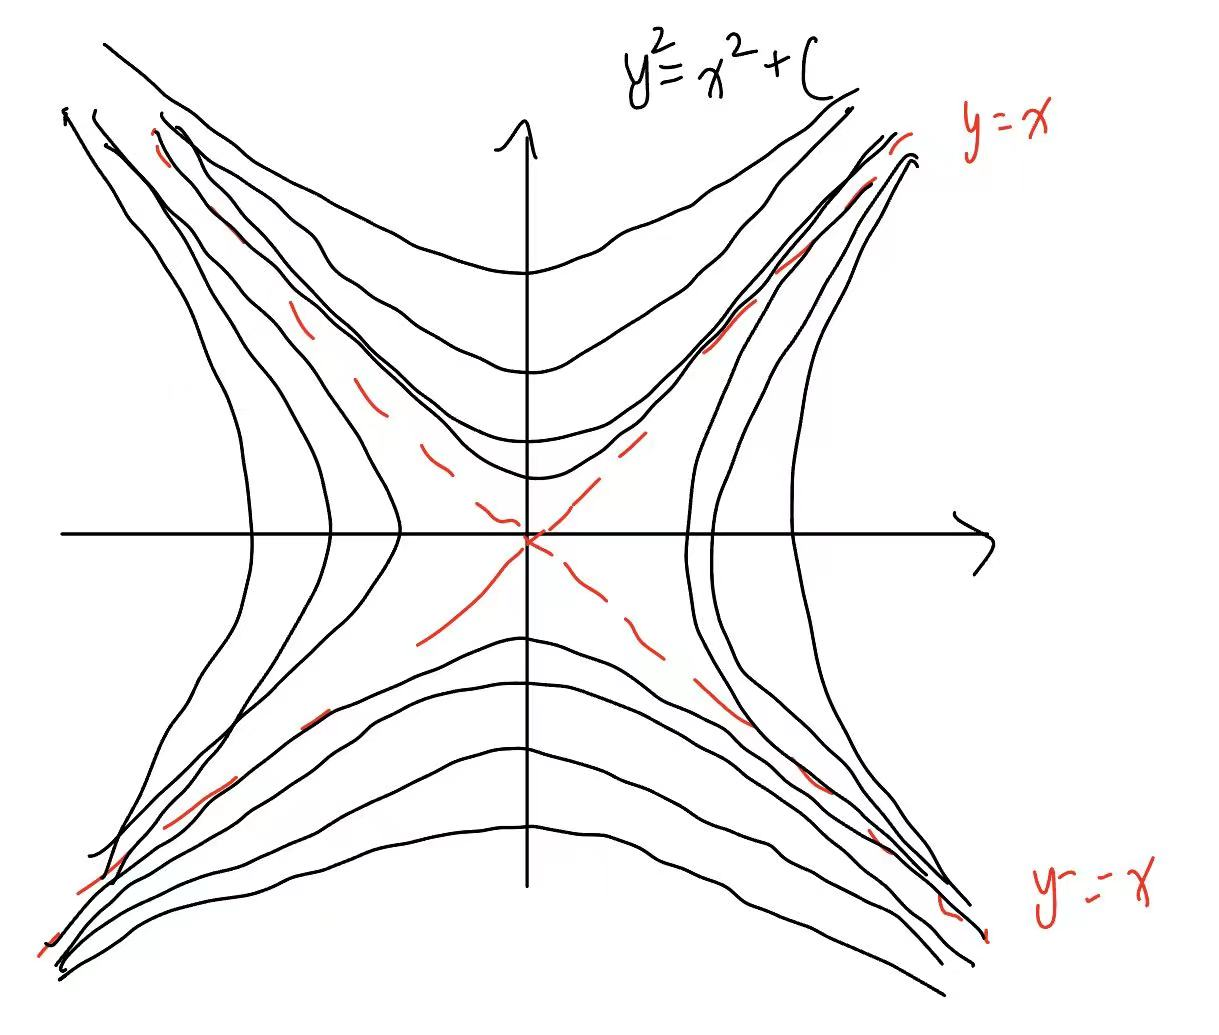
\includegraphics[width=10cm]{DE-ch2-7-1.jpg}
\end{figure*}
\\
This plot is symmetrical across both axes as expected, and asymptotically approaches $y=\pm x$.
\\
\\
For the second DE, consider the given substitution and differentiate both sides:
\begin{equation*}
    \begin{aligned}
        y &= \log u - x \\
        \frac{dy}{dx} &= \frac{1}{u}\frac{du}{dx} - 1 \\
        \frac{du}{dx} &= u(1+\frac{dy}{dx}) 
    \end{aligned}
\end{equation*}
Substituting into the DE thus yields
\begin{equation*}
    \begin{aligned}
        uy(1+\frac{dy}{dx}) - u \log u &= 0 \\
        y(1+\frac{dy}{dx}) - \log u &= 0 \\
        y(1+\frac{dy}{dx}) - (\log u - x) &= x \\
        y(1+\frac{dy}{dx}) - y &= x \\
        y\frac{dy}{dx} &= x
    \end{aligned}
\end{equation*}
which matches the first DE. Thus the solutions to $y = \log u - x$ is $y = \pm \sqrt{x^2+C}$, giving $u = e^{y+x} = e^{x \pm \sqrt{x^2+C}}$ for some constant $C$. To plot these solutions, we consider the cases $u = e^{x+\sqrt{x^2+C}}$ and $u=e^{x-\sqrt{x^2+C}}$.\\ \\ 
In the first case, when $C = 0$, $y = x$ and thus $u$ is mapped to $e^{2x}$, which serves as the asymptote for this family of curves. The end behavior of this curve family tends to $1$ as $x$ tends to $-\infty$ as $x$ and $\sqrt{x^2+C}$ will have similar magnitudes but opposite signs, and tends to $e^{2x}$ as $x$ tends to $\infty$ as $\sqrt{x^2+C}$ approaches $x$. It is also worth considering the domain of $y$ when $C$ is negative. A graph of some solution curves are shown below:
\begin{figure*}[h]
    \centering
    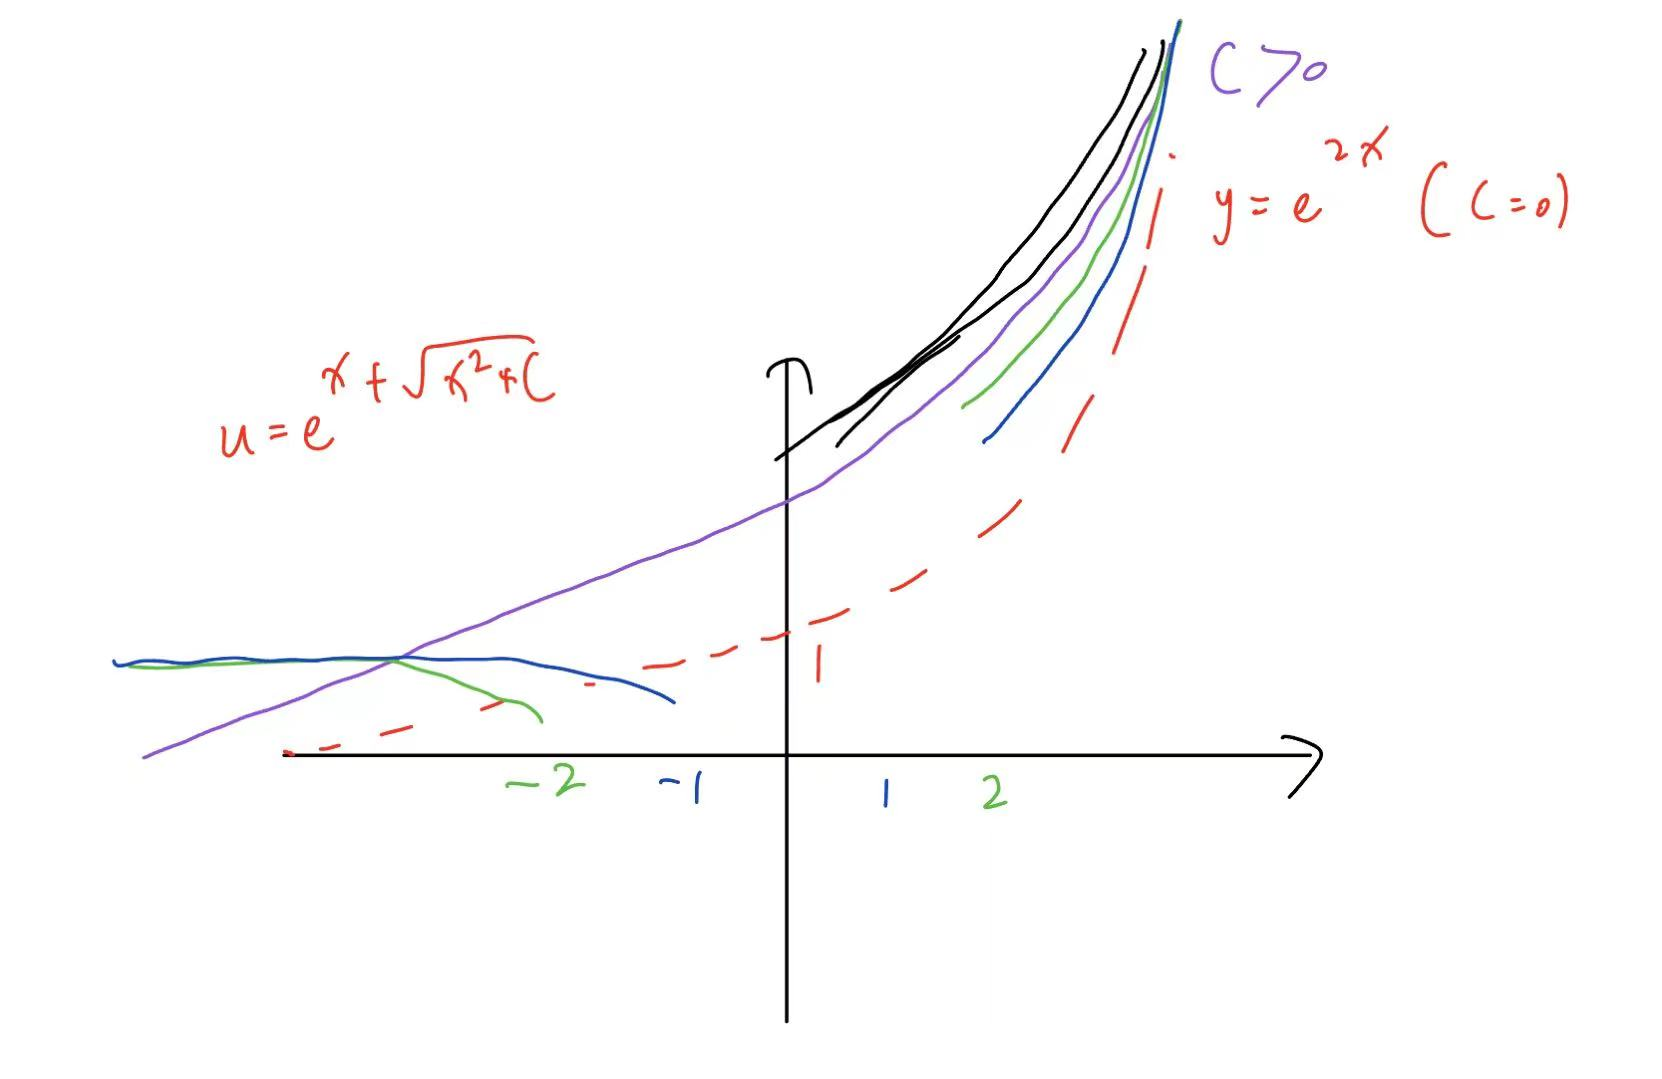
\includegraphics[width=10cm]{DE-ch2-7-3.jpg}
\end{figure*}\\
As shown, curves with $C>0$ are defined for all $x$ and approach $y=e^{2x}$ from above (as they are always larger than $y=e^{2x}$); curves with $C<0$ will not be defined between a certain range ($C=-4, -1$); all curves in the family will approach $y=1$ as $x$ approaches $-\infty$. A similar approach can be used to plot the family $u=e^{x-\sqrt{x^2+C}}$, as shown below:
\begin{figure*}[h]
    \centering
    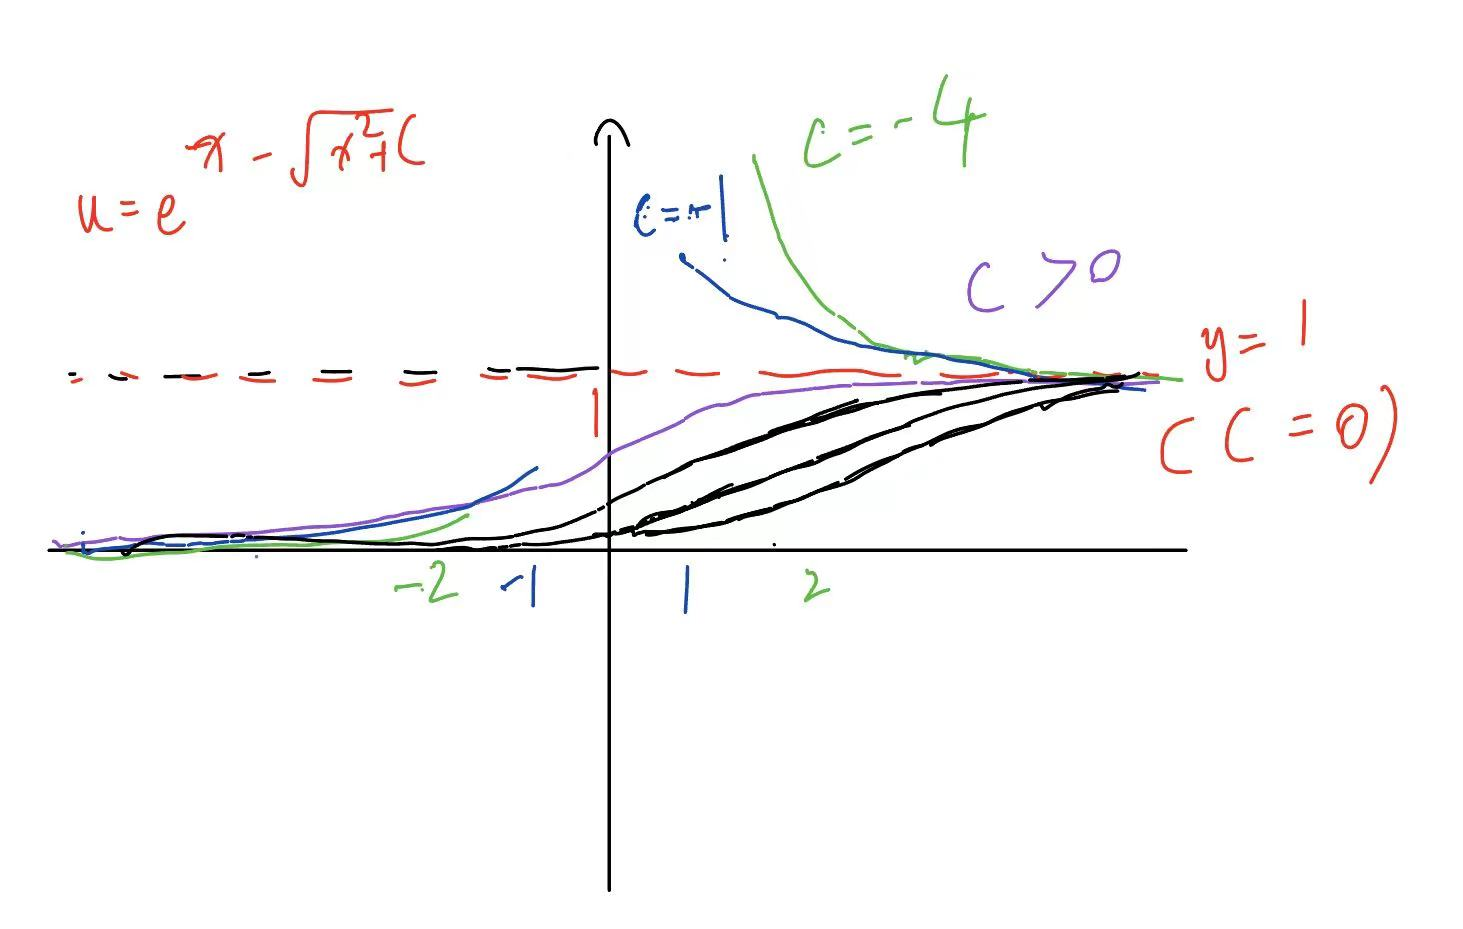
\includegraphics[width=10cm]{DE-ch2-7-2.jpg}
\end{figure*}\\
The same characteristics are present on this graph, but with an asymptote to $y=1$ as when $C=0$, $u=e^{x-x}=1$, and with curves approaching $y=0$ as $x$ approaches $-\infty$. The same discontinuities appear as in the above case.
\hrulefill

\subsubsection*{In each of the following, sketch a few solution curves: (i) $y'+xy=1$, (ii) $y' = x^2+y^2$, (iii) $y'=(1-y)(2-y)$.}
\bf (i) Solution. \normalfont We note a few features of the solution curves that satisfy $y' + xy = 1$:
\begin{enumerate}
    \item Their slopes are all equal to 1 on the x- and y-axes, as $1-xy$ equals 0 when $x = 0$ or $y=0$.
    \item $y'$ is positive in the second and fourth quadrants.
    \item All critical points where $y' = 0$ lie on $xy = 1$, or $y=\frac{1}{x}$.
\end{enumerate}
Thus a plot of the solution curves is shown here (in purple and yellow), with the isocline $y' = -1, xy = 2$ shown:
\begin{figure*}[h]
    \centering
    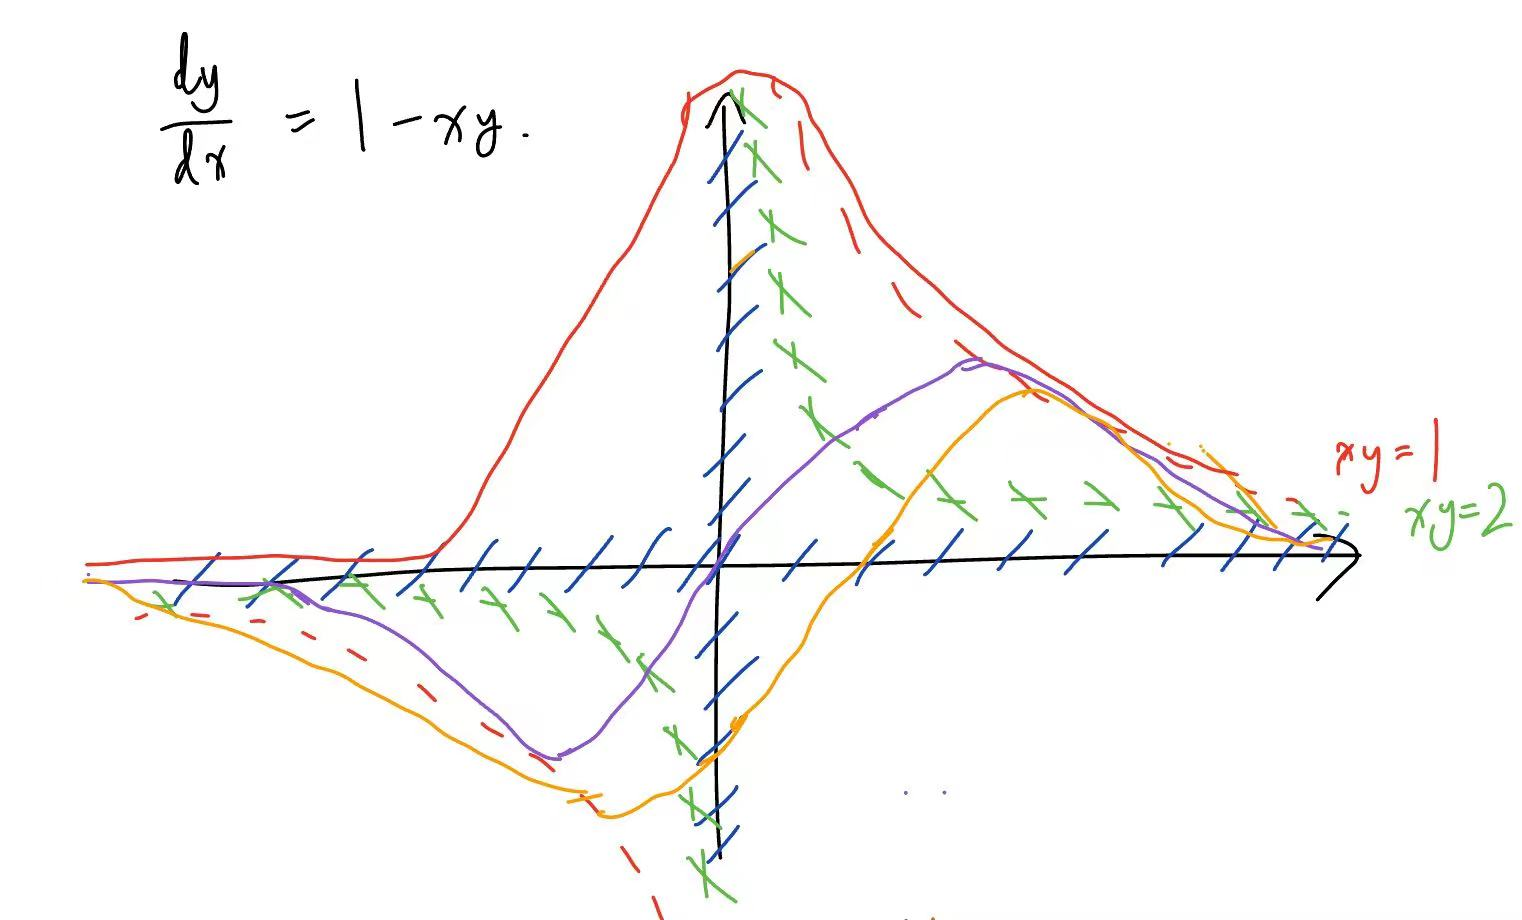
\includegraphics[width=10cm]{DE-ch2-8-1.jpg}
\end{figure*}\\
\bf (ii) Solution. \normalfont The expression $y' = x^2 + y^2$ indicates that the isoclines of $y$ lie on circles with varying radius, and that the slope of $y$ is always non-negative; as $y'$ is an even function, $y$ is an odd function and thus passes through the origin. The origin has $y' = 0^2 + 0^2 = 0$, but the sign of the gradient does not change (is always positive); thus, the origin is an inflection point. A plot of solution curves is shown below:
\begin{figure*}[h]
    \centering
    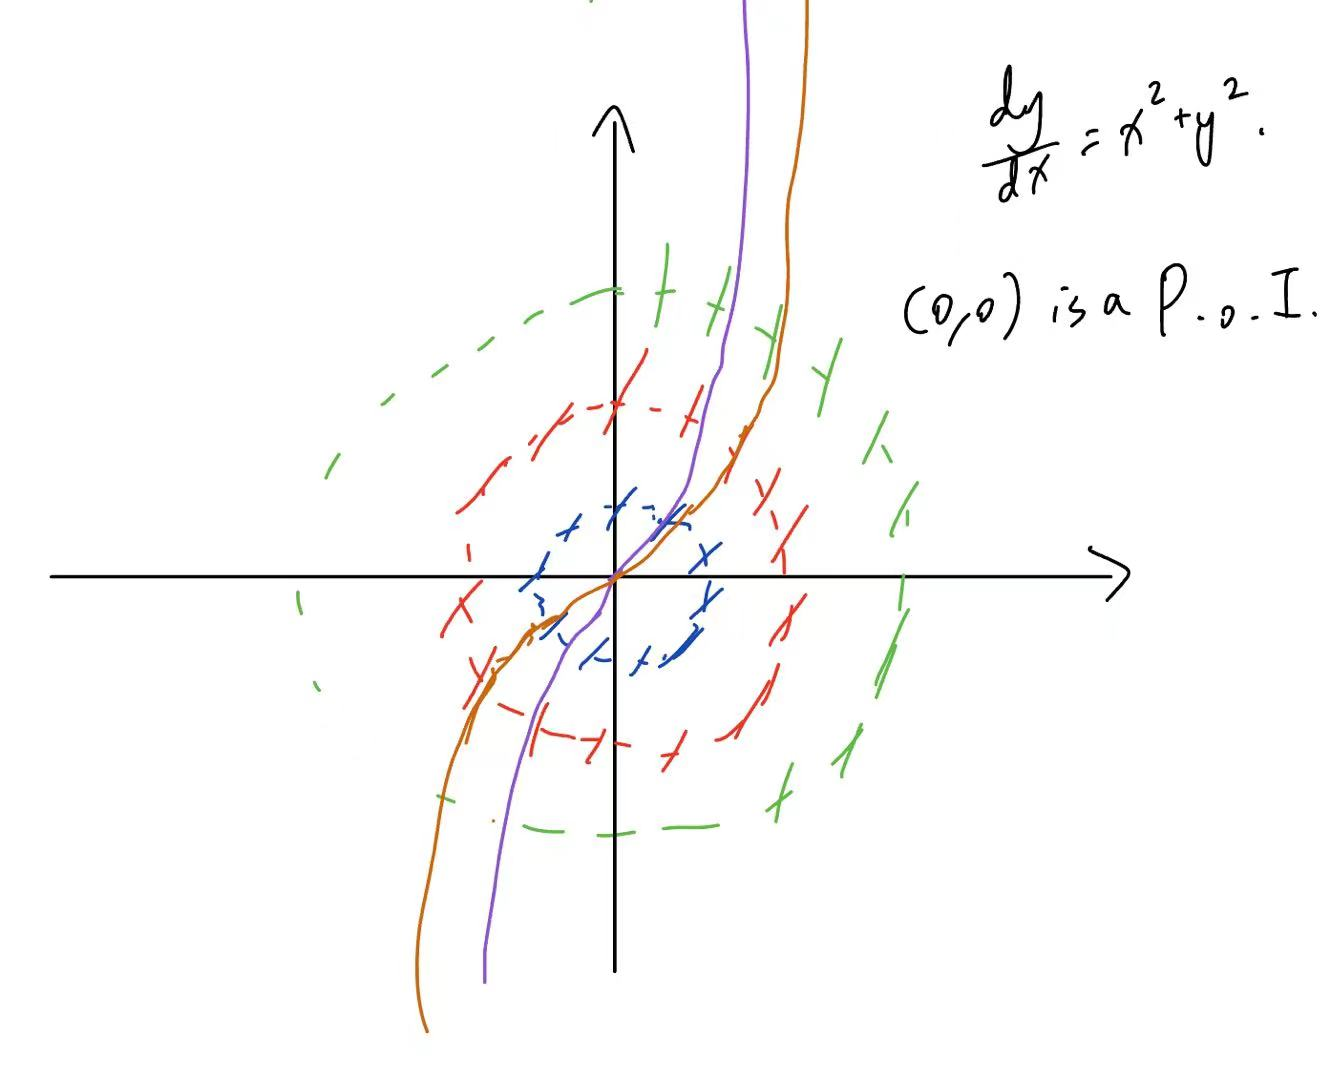
\includegraphics[width=10cm]{DE-ch2-8-2.jpg}
\end{figure*}\\
\bf (iii) Solution. \normalfont $y' = (y-1)(y-2)$ is an autonomous equation; it is clear that $y = 1$ and $y=2$ with $y'=0$ are constant solutions to this DE. Thus, we conduct stability analysis on these fixed points. For $y = 1$, let $\epsilon$ be an arbitrarily small perturbation and set $y* = 1+ \epsilon$. Thus
\begin{equation*}
    \begin{aligned}
        \frac{dy*}{dx} &= \frac{d\epsilon}{dx} \\
        &= (y-1)(y-2),\ y=1+\epsilon \\
        &= (y-1)(y-2) + \epsilon \frac{d}{dx} (y-1)(y-2),\ y=1
    \end{aligned}
\end{equation*}
by Taylor expansion, where the final line evaluates to $-\epsilon$. Thus $\frac{d\epsilon}{dx} = -\epsilon$, and $\epsilon = Ae^{-x}$ for some $A$, meaning that it approaches 0 as $x$ approaches $\infty$. A similar analysis on the fixed point $y=2$ yields that any perturbation diverges to $\infty$ as x approaches $\infty$, being on the order $\epsilon = Ae^x$. Thus $y=2$ is an unstable fixed point while $y=1$ is stable. Observe also that below the line $y=1$ or above $y=2$, $\frac{dy}{dx}$ is positive, while in-between the two, $y$ is negative. We arrive at the following plot:
\newpage
\begin{figure*}[h]
    \centering
    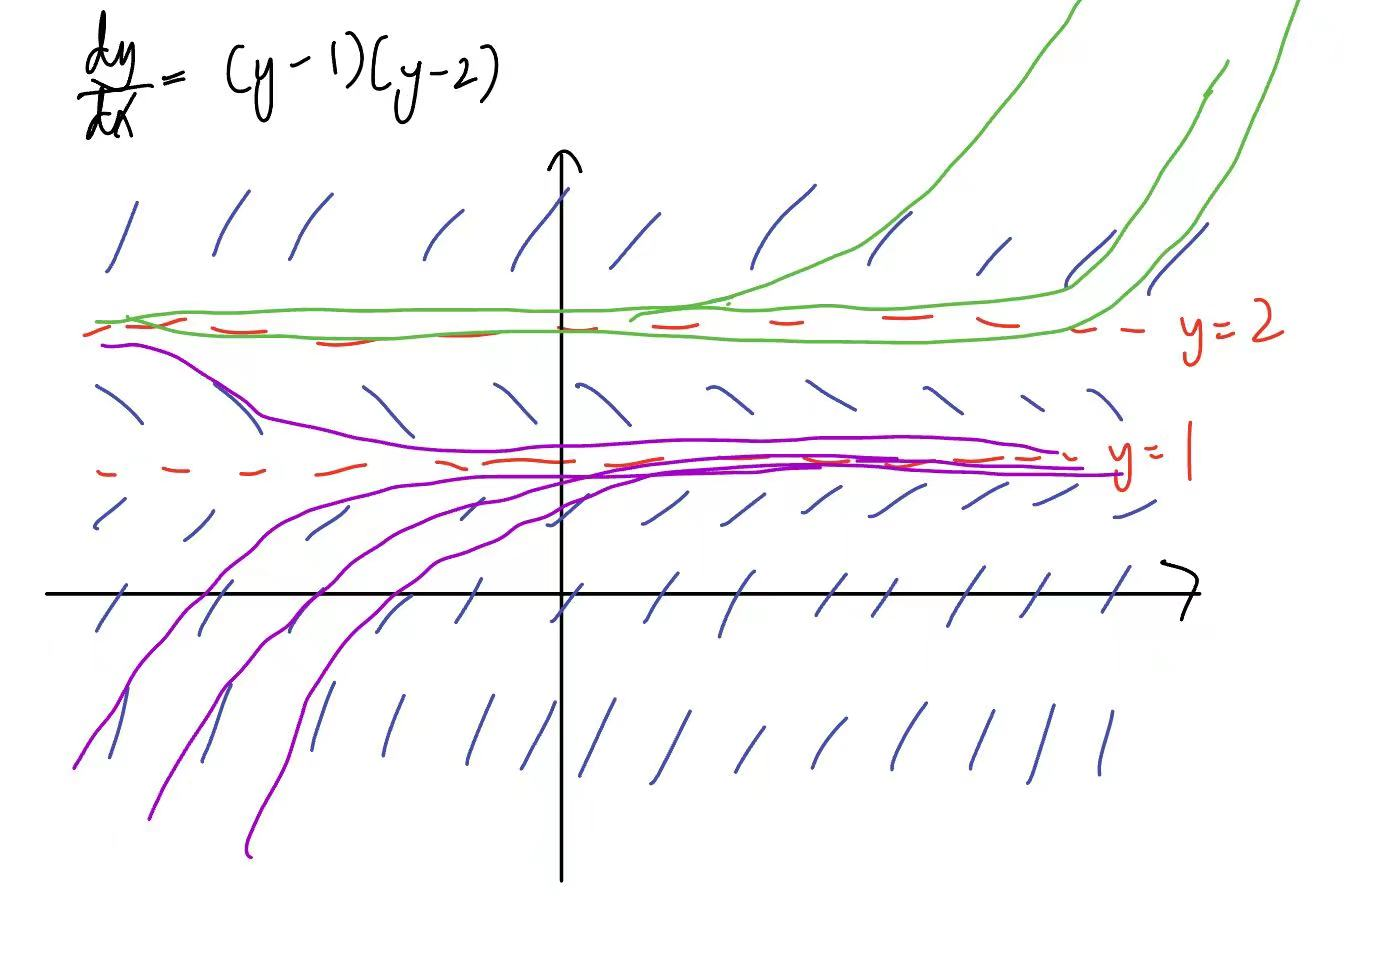
\includegraphics[width=10cm]{DE-ch2-8-3.jpg}
\end{figure*}
Note that the slope is the same when $y$ is held constant. Purple indicates curves converging towards $y=1$, while green indicates curves diverging from $y=2$.\\

\hrulefill

\subsubsection*{(i) Sketch the solution curves for $\frac{dy}{dx}=xy$. Find the family of solutions determined by this equation and reassure yourself that your sketches were appropriate. 
\\ \\ (ii) Sketch the solution curves for $\frac{dy}{dx} = \frac{x-y}{x+y}$. By rewriting the equation as $(x\frac{dy}{dx}+y)+y\frac{dy}{dx}=x$, find and sketch the family of solutions.}
\bf (i) Solution. \normalfont We note that $\frac{dy}{dx} = xy$ has all its critical points on the axes; $\frac{dy}{dx}$ is reflectively symmetrical across both axes (meaning that $y$ itself is an even function), and $\frac{dy}{dx} = k$ lies on the curve $y = \frac{k}{x}$. This gives us enough information to sketch a graph:\\
\begin{figure*}[h]
    \centering
    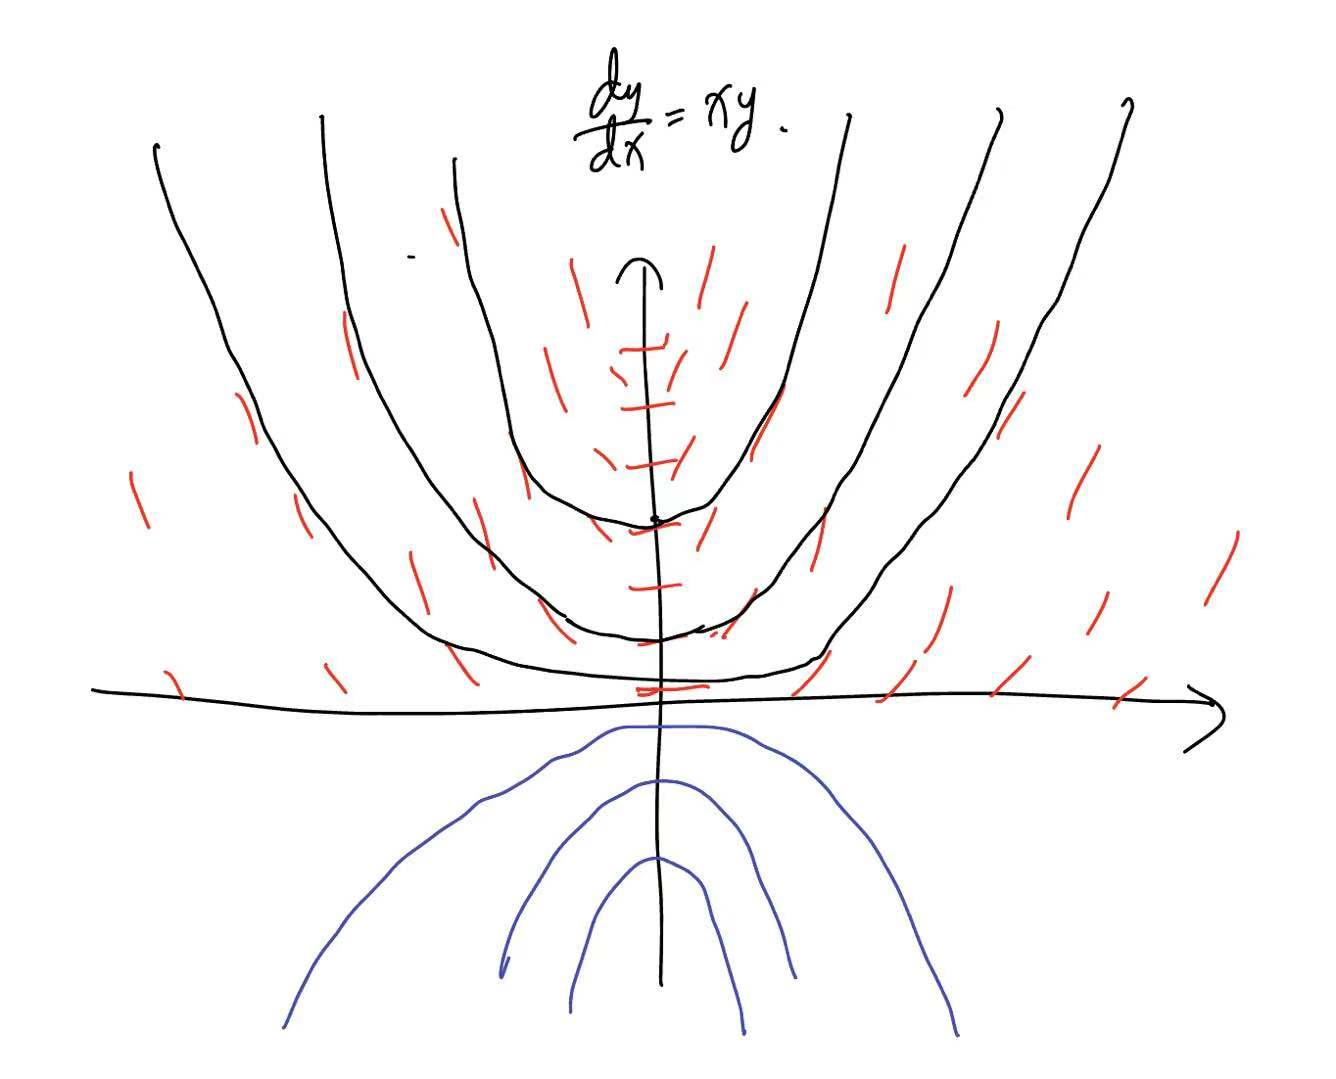
\includegraphics[width=8cm]{DE-ch2-9-1.jpg}
\end{figure*}\\
The family of solutions determined by this DE can be found analytically:
\begin{equation*}
    \begin{aligned}
        \frac{dy}{dx} &= xy \\
        \int \frac{dy}{y} &= \int x\ dx \\
        \ln y &= \frac{x^2}{2} + C \\
        y &= Ae^{\frac{x^2}{2}}
    \end{aligned}
\end{equation*}
for some constant $A$, which exhibits all the features required on the graph (minima on the y-axis, even function, exponential growth).
\\
\\
\bf (ii) Solution. \normalfont Note that the critical points of $\frac{dy}{dx} = \frac{x-y}{x+y}$ lie on $x-y = 0$, or the line $x=y$. The gradient is infinite at $x+y = 0$, or the line $x = -y$. $\frac{dy}{dx}$ is symmetrical about the origin. The $y$-axis represents $y' = 1$, while the $x$-axis represents $y' = -1$; the gradient at the origin is not defined. 
\\
\\
The isocline $y' = a$ for some $a$ is given by $y = -\frac{a-1}{a+1}x$. When $a \to 0^+$, the isocline approaches $y = x$ from the left side, and when $a \to 0^-$ the isocline approaches $y=x$ from the right side. To the left of $y = x$, the slope field will gradually steepen positively, and to the right of $y=x$, the slope field will gradually steepen negatively. This gives us enough information to sketch a graph:
\begin{figure*}[h]
    \centering
    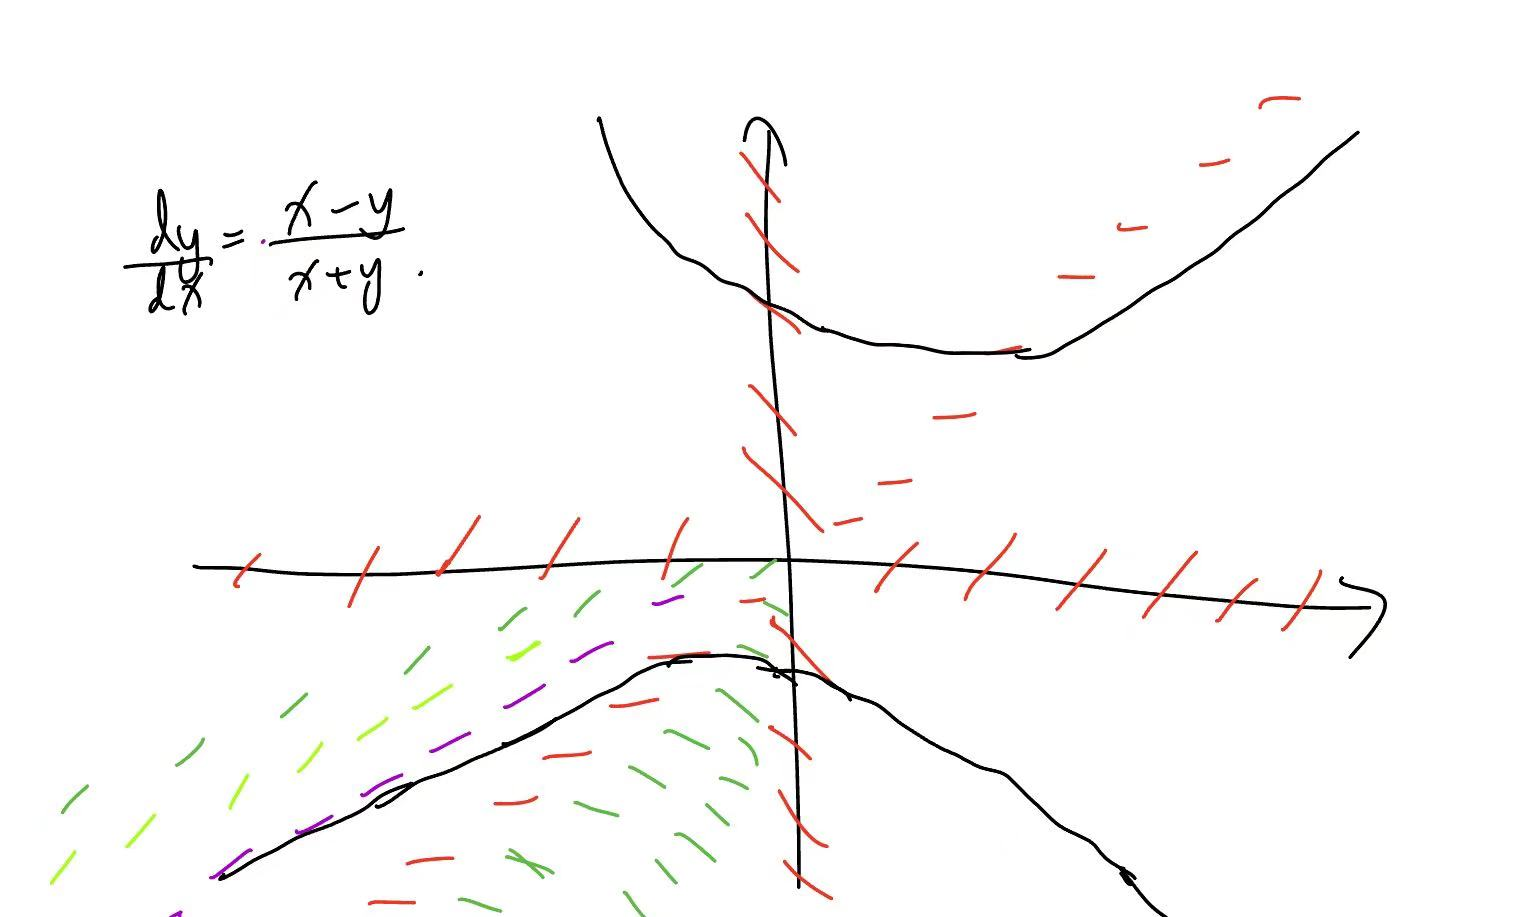
\includegraphics[width=10cm]{DE-ch2-9-2.jpg}
\end{figure*}\\
Note the symmetry of the solution curves about the origin due to the symmetry of $y'$ (proof by assumption). As the question hints at, we rewrite the equation in an attempt to obtain analytic solutions:
\begin{equation*}
\begin{aligned}
\frac{dy}{dx} &= \frac{x-y}{x+y} \\
(x+y)dy &= (x-y)dx \\
(y-x)dx + (x+y)dy &= 0 \\
\end{aligned}
\end{equation*}
Using exact differentials, we let the solution to the DE be $f$ and set $P = \frac{\partial f}{\partial x} = y-x, Q = \frac{\partial f}{\partial y} x+y$, confirming that $P_y=Q_x=1$. 
We then have:
\begin{equation*}
    \begin{aligned}
    f(x,y) = \int \frac{\partial f}{\partial x}\ dx &= \int P\ dx \\
    &= \int y-x\ dx \\
    &= xy - \frac{x^2}{2} + h(y)\ \text{for some $h(y)$ depending only on $y$} \\
    \\
    \frac{\partial}{\partial y} f(x,y) &= Q \\
    &= x + h'(y) \\
    &= x + y \\
    \\
    h'(y) &= y \\
    h(y) &= \frac{y^2}{2} \\
    f(x,y) &= xy - \frac{x^2}{2} + \frac{y^2}{2}
    \end{aligned}
    \end{equation*}
which yields solutions $f(x,y)=xy-\frac{x^2}{2}+\frac{y^2}{2}=k$ for some constant $k$, or $y^2 + 2xy - (x^2 + k) = 0$, giving $y = -x \pm \sqrt{2x^2 + k}$ (jumping through several hoops of simplication with the quadratic formula). This curve is asymptotic to $(\pm\sqrt{2}-1)x$ and will have a turning point due to the symmetry of $x^2$. A rough plot of the solution curves appears as follows:
\begin{figure*}[h]
    \centering
    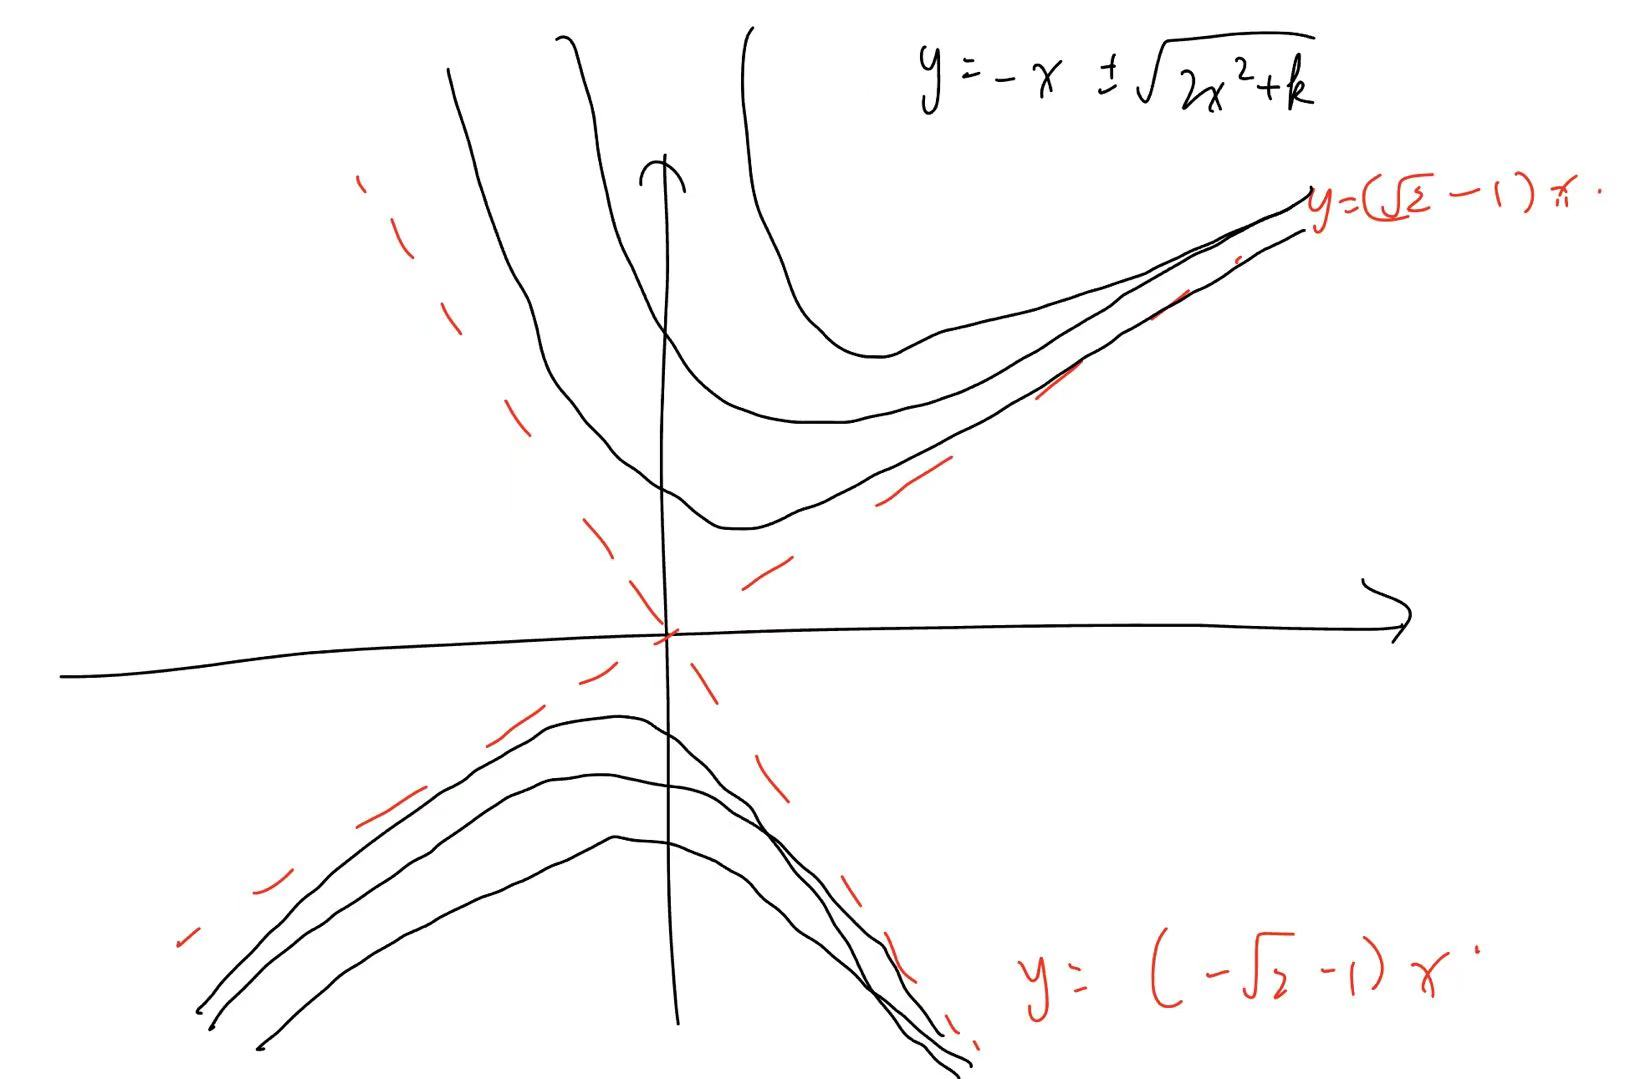
\includegraphics[width=10cm]{DE-ch2-9-3.jpg}
\end{figure*}\\
note that the bottom branch is always negative, while the top branch is always positive.

\hrulefill

\subsubsection*{Measurements on a yeast culture have shown that the rate of increase of the biomass of yeast is related to the biomass itself by the equation \begin{equation*}
    \frac{dN}{dt} = aN - bN^2
\end{equation*}
    where N(t) is a measure of the biomass at time $t$, and $a$ and $b$ are positive constants. Without solving the equation, find in terms of $a$ and $b$: \\ \\
    (i) the value of $N$ at which $\frac{dN}{dt}$ is a maximum; \\
    (ii) the values of $N$ at which $\frac{dN}{dt}$ is zero, and the corresponding values of $\frac{d^2 N}{dt^2}$. \\ \\
    Using all this information, sketch the graph of $N(t)$ against $t$, and compare this with what you obtain by solving the equation analytically for $0 \leq N \leq \frac{a}{b}$.
}
\bf (i) Solution. \normalfont $aN-bN^2$ is a quadratic function in $N$ with vertex at $N = \frac{-a}{-2b} = \frac{a}{2b}$. This is the sole maximum because the coefficient of $N^2$ is negative.
\\ \\
\bf (ii) Solution. \normalfont Simply factoring obtains $N(a-bN)=0$, or $N=0$ and $N=\frac{a}{b}$. $\frac{d^2N}{dt^2}$ can be obtained by differentiating $\frac{dN}{dt}$ with respect to $t$, which is $a \frac{dN}{dt} - 2bN\frac{dN}{dt} = (a-2bN)(aN-bN^2)$ by substituting the original DE. Thus, the values of $N$ at which the second derivative is 0 are $N=0, \frac{a}{b}$, and $\frac{a}{2b}$. It is worth noting that $N=\frac{a}{2b}$ represents both a maximum and a point of inflection, as the second derivative changes sign at that point (proof: just trust me). 
\\ \\
From the above two sections, and combined with the fact that the DE for $N$ is an autonomous equation, we now know that the points for which $\frac{dN}{dt} = 0$ - $N = 0$ and $\frac{a}{b}$ - are fixed points, and solutions to the DE; a stability analysis on both points (which would likely put the author into some sort of boredom-induced coma if written in full) reveals that small perturbations $\epsilon$ near the two fixed points have $\frac{d\epsilon}{dt} \approx \epsilon \frac{\partial}{\partial N }(aN - bN^2) = a - 2bN$; thus, the fixed point $N=0$ has $\frac{d\epsilon}{dt} = a > 0$ and is unstable, while $N=\frac{a}{b}$ has $\frac{d\epsilon}{dt} = -a <0$ and is stable (perturbation converges to 0). \\ \\
We further note that a point of inflection lies at the maximum of $\frac{dN}{dt}$, or $N = \frac{a}{2b}$. This gives us enough information to plot a graph:
\begin{figure*}[h]
    \centering
    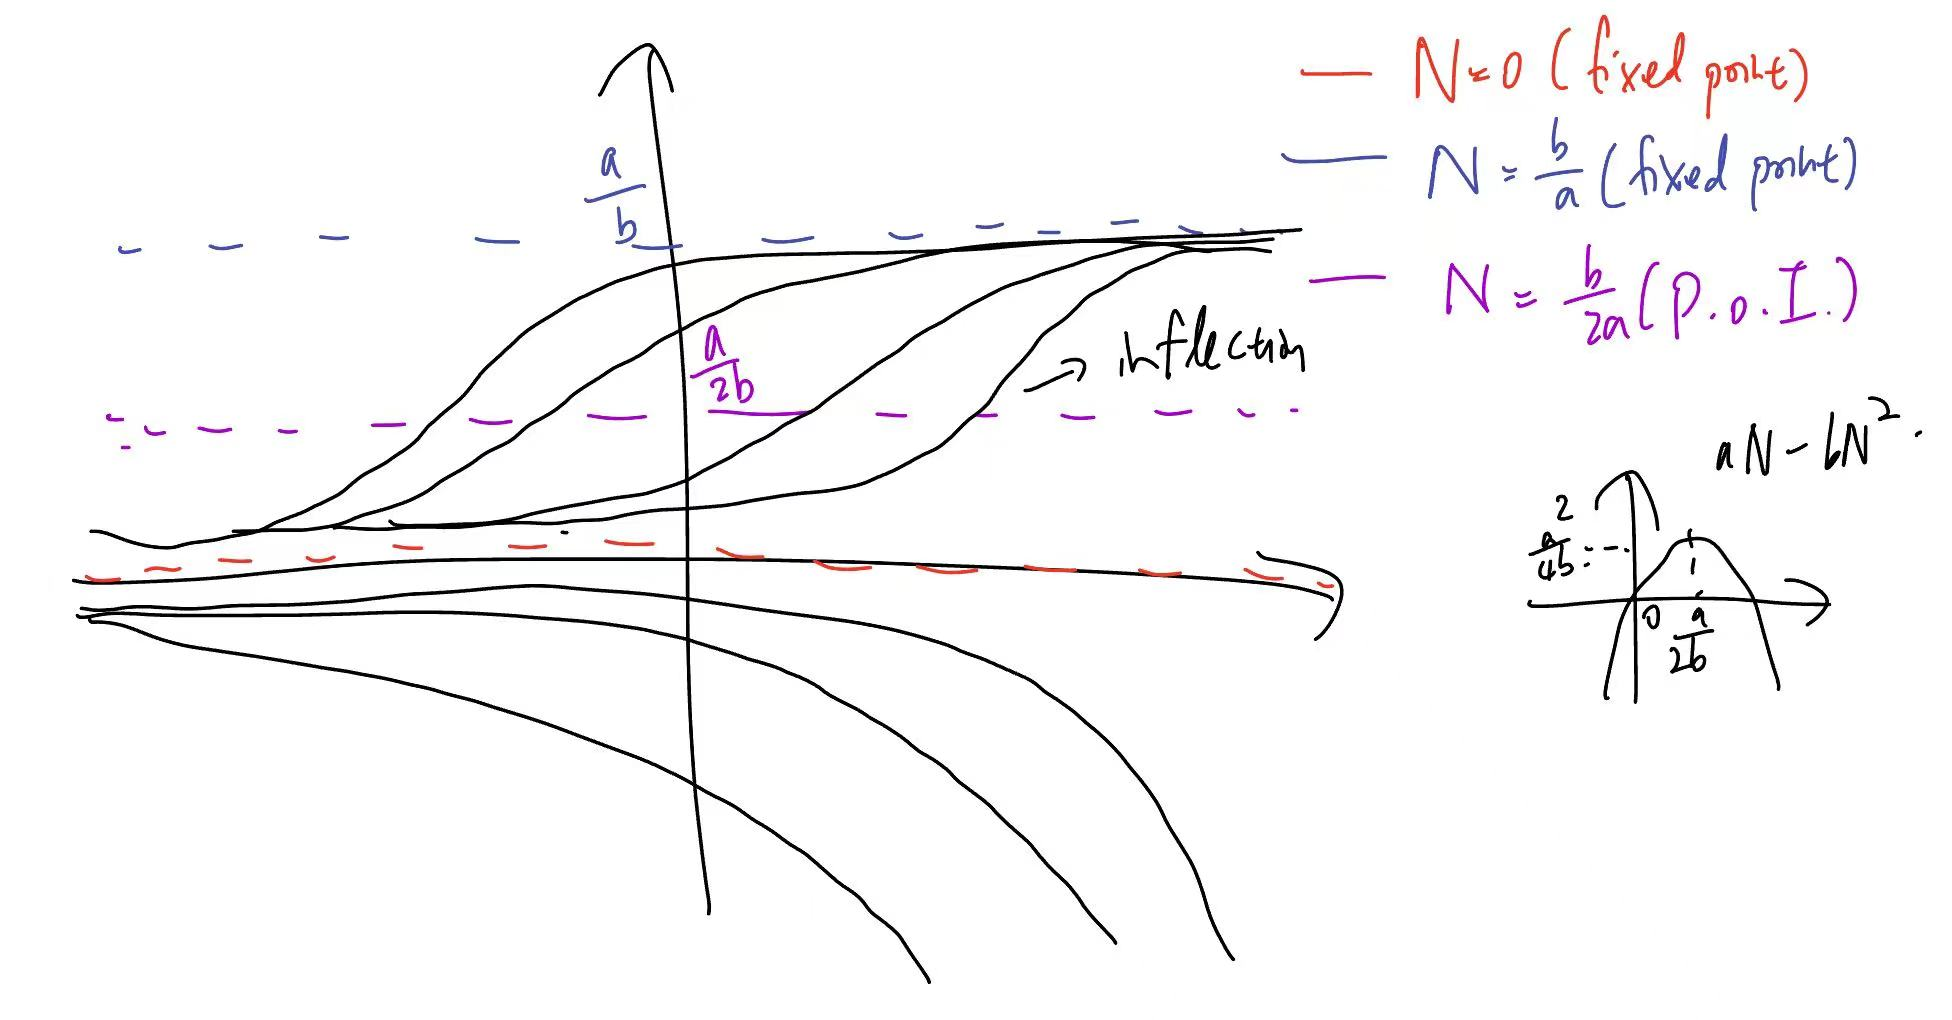
\includegraphics[width=11cm]{DE-ch2-10-1.jpg}
\end{figure*}\newpage
$\frac{dN}{dt}$ is positive at $0<N< \frac{a}{2b}$ and exactly zero at $N=0$; thus, for solutions slightly smaller than 0 initially, the solution curve will diverge to negative infinity, while solutions slightly greater than 0 will converge to the fixed point $N=\frac{a}{b}$. These convergent solutions have a point of inflection at $N=\frac{a}{2b}$. (NOTE: there should be a solution curve above $N = \frac{a}{b}$ as well, but I'm dumber than a sack of volcanic rocks, so I forgot.)\\ \\
An analytic solution of the DE obtains $\frac{dN}{aN-bN^2} = dt$, in which the left-hand side equals $\frac{1}{a}(\frac{1}{N}+\frac{b}{a-bN})\ dN$ by partial fractions; integrating both sides yields $\frac{1}{a}(\ln N - \ln (a - bN)) = t + C$ for some $C$, or $\ln \frac{N}{a-bN} = at + C, \frac{N}{a-bN} = Ae^{at}, (1+bAe^{at})N = aAe^{at}, N = \frac{ae^{at}}{A+be^{at}}$. This is a logistic curve that yields the same graph as the sketch. \\

\hrulefill

\subsubsection*{Water flows into a cylindrical bucket of depth $H$ and cross-sectional area $A$ at a volume flow rate $Q$ which is constant. There is a hole in the bottom of the bucket of cross-sectional area $a << A$. When the water level above the hole is $h$, the flow rate out of the hole is $a\sqrt{2gh}$, where $g$ is the gravitational acceleration. Derive an equation for $\frac{dh}{dt}$. Find the equilibrium depth $h_e$ of water, and show that it is stable.}
An (extremely accurate, very artistically valuable, supremely well-drawn and masterful) picture of the problem's conditions is shown below:
\begin{figure*}[h]
    \centering
    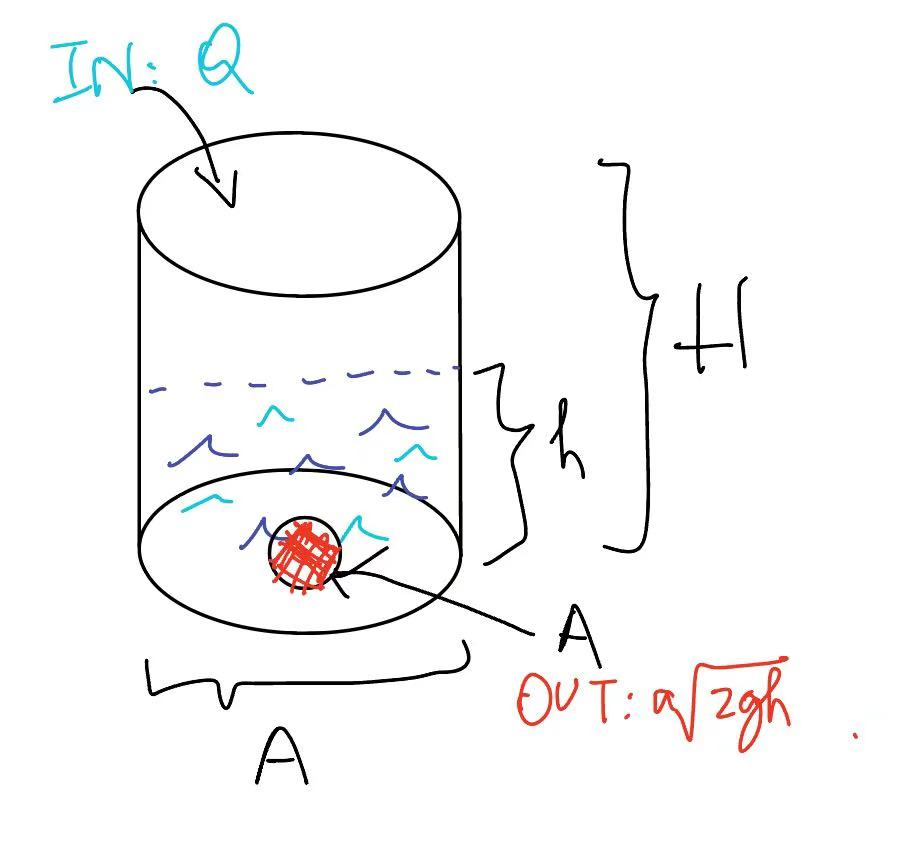
\includegraphics[width=10cm]{DE-ch2-11-1.jpg}
\end{figure*}\\
Let the volume of water in the bucket at a time $t$ be $V(t)$; $V$ is related to $h(t)$, the water level, by a constant multiple: $V = h(A-a)$ (the area of the donut shape that comprises the bottom of the bucket. Yes, I'm calling it a donut.) The rate of water flowing into the bucket is $Q$ while the rate of water flowing out is $a\sqrt{2gh}$; thus, we write $\frac{dV}{dt} = \frac{dh(A-a)}{dt} = Q-a\sqrt{2gh}$. All of $A, a, Q, g$ are constants, so we have $\frac{dh}{dt} = \frac{Q-a\sqrt{2gh}}{A-a}$. 
 Note that this is an autonomous DE in $h$, so we set $\frac{dh}{dt} = 0$ to obtain $Q-a\sqrt{2gh} = 0,\ h_e = \frac{Q^2}{2ga^2}$ as a fixed point and solution of the DE (equilibrium depth). \\ \\
To show that $h_e$ is stable, we conduct stability analysis and note that any small perturbation $\epsilon$ near $h_e$ will have $\frac{d\epsilon}{dt} = \epsilon (\frac{d}{dh}\frac{dh}{dt}) = \epsilon\frac{-ga}{(A-a)\sqrt{2gh}}$. At $h = h_e$, this is $\frac{d\epsilon}{dt} = \epsilon\frac{-ga}{(A-a)\sqrt{2g \frac{Q^2}{2ga^2}}} = \epsilon\frac{-ga}{(A-a)\sqrt{\frac{Q^2}{a^2}}} = \epsilon\frac{-ga^2}{(A-a)Q}$. All of the constants in this equation are positive ($g = 10$, please don't murder me in my sleep physicists; $A-a > 0$ as $A >> a$; $a^2 > 0$) and thus $\frac{d\epsilon}{dt}$ is a negative constant multiple of $\epsilon$, which yields an exponentially decaying form for $\epsilon$. This shows that $h_e$ is a stable equilibrium.

\hrulefill

\subsubsection*{In each of the following equations for $y(t)$, find the equilibrium points and classify their stability properties: \\ \\
(i) $\frac{dy}{dt} = y(y-1)(y-2)$ \\ \\
(ii) $\frac{dy}{dt} = -2\tan^{-1}[\frac{y}{1+y^2}]$ \\ \\
*(iii) $\frac{dy}{dt} = y^3(e^y-1)^2$.
}
\bf (i) Solution. \normalfont See Example 2.25 in the stability analysis section. \\ \\
\bf (ii) Solution. \normalfont This is an autonomous equation, so the constant values of $y$ for which $-2\tan^{-1}[\frac{y}{1+y^2}] = 0$ are also constant solutions to the DE. These values of $y$ are where $\frac{y}{1+y^2} = 0$, or $y = 0$. At the fixed point $y^* = 0$, a small perturbation $\epsilon$ has $\frac{d\epsilon}{dt} \approx \epsilon \frac{d}{dy}(-2\tan^{-1}\frac{y}{1+y^2})$
= $-2\epsilon(\frac{d}{dy} \frac{y}{1+y^2})(\frac{1}{1+(\frac{1}{1+y^2})^2})$. As $y=0$, the final term is $\frac{1}{2}$; $\frac{d}{dy}\frac{y}{1+y^2} = \frac{(1+y^2)-2y^2}{(1+y^2)^2}$, which equals 1 when $y=0$. Thus, $\frac{d\epsilon}{dt} = -2\epsilon(1)(\frac{1}{2}) = -\epsilon$, making the fixed point stable. \\ \\
\bf (iii) Solution. \normalfont The fixed point of $\frac{dy}{dt}$ is $y=0$ (as $e^y-1 = 0$ and $y^3 = 0$). (This fixed point gives $\frac{d\epsilon}{dt} = 0$ and I don't know what to do HELP) (try taylor expansions beyond the $O(\epsilon)$ term?)

\hrulefill

\subsubsection*{Investigate the stability of the fixed points of the difference equation
\begin{equation*}
    u_{n+1} = 4u_n(1-u_n).
\end{equation*}
In the case $0\leq u_n \leq 1$, use the substitution $u_0 = \sin^2 \theta$ to find the general solution and verify your stability results. Can you find an explicit form of the general solution in the case $u_0 > 1$?
}
\bf Solution. \normalfont Short answer: yes. Long answer: yyyyyyyyyes.\newpage A \textit{fixed point} of a difference equation is a point $u_n$ such that $u_{n+1}=u_n$, thereby making all following terms equal to $u_n$ as well (the sequence is "fixed" at that value). If a certain $u_n = u^*$ satisfies this property, then we have $u_{n+1} = 4u^*(1-u^*) = u^*$, which yields $3u^*=4(u^*)^2$ - a quadratic in $u^*$ with solutions $u^* = 0, \frac{3}{4}$. \\ \\
To investigate the stability of these fixed points, we employ a similar method to that of DEs: let $\epsilon$ represent a small perturbation from the fixed point $u^*$ and consider the value of $u_{n+1}$ if $u_n$ instead equaled $u^* + \epsilon_n$. Denote $u_{n+1}$ by $f(u_n)$; also let $u_{n+1}$ equal $u_n + \epsilon_{n+1}$, where $\epsilon_{n+1}$ is the perturbation of $u_{n+1}$ away from the fixed point $u_n$ that we are trying to find. At $u_n = u^* + \epsilon$, $u_{n+1} = u_n + \epsilon_{n+1} = f(u^* + \epsilon) \approx f(u^*) + \epsilon_n f'(u^*)$; as $u^*$ is a fixed point, $f(u^*) = u_n$ and so $\epsilon_{n+1} \approx \epsilon_n f'(u^*)$. This is analogous to the perturbation theorem for differential equations, and yields that $\epsilon_{n} = \epsilon_0 [f'(u^*)]^n$ due to it following a geometric progression, for some initial perturbation $\epsilon_0$. As such, if $|f'(u^*)| > 1$ the perturbation diverges with an unstable fixed point, and if $|f'(u^*)| < 1$ it converges and the fixed point is stable. Applying this statement to the fixed points $u^* = 0, \frac{3}{4}$ with $f'(u^*) = 4 - 8u^*$ yields instability for both points. 
\\ \\
To verify this, we use the suggested substitution $u_0 = \sin^2 \theta$, which fully encompasses the range $0 \leq u_0 \leq 1$. Substituting into the recurrence relation gives $u_1 = 4u_0(1-u_0) = 4\sin^2 \theta (1-\sin^2 \theta) = 4\sin^2 \theta \cos^2 \theta = (2\sin \theta \cos \theta)^2 = \sin^2 (2\theta)$. Induction would show that $u_n$ has general formula $\sin^2 (2^n \theta)$. The proof is as follows:
\begin{proof}
    Obvious.
\end{proof}
This shows that any value of $u_0$ between 0 and 1, besides the two fixed points, are unstable; the value of $\sin(2\theta)$ will fluctuate quasi-periodically with no clear pattern and the sequence will not converge to a certain value. This verifies that both fixed points are unstable.
\\ \\
To proceed with an explicit form of the general solution when $u_0 > 1$, consider a hyperbolic substitution like $u_n = -\sinh^2 \theta$, encompassing all the positive reals exceeding 1. This would make $u_{n+1} = -4\sinh^2 \theta(1+\sinh^2 \theta) = -4\sinh^2 \theta \cosh^2 \theta = -\sinh^2 (2\theta)$, and once again, we find that the general term $u_n$ is $-\sinh^2(2^n \theta)$ with $\theta$ previously defined. The proof is as follows:
\begin{proof}
    Elementary. (Not really, but I'm really lazy ;-;)
\end{proof}
This would require a complex value of $\theta$, but the resulting $u_n$ is real so there probably won't be a problem. (Witness the incredible power of "proof by handwaving".)

\section{Second-order differential equations}
\begin{definition}
A \it{second-order}\normalfont  ordinary differential equation in $x$ and $y$ is one whose highest-order derivative of $y$ is the second derivative. Most methods that apply to second-order ODEs also apply to higher-order equations as well. \\ \\
A \it{linear} \normalfont  second-order ODE is one that does not have any higher powers of $y, y', y''$ beyond the 1st power. As non-linear second-order ODEs are difficult to discuss analytically, the following sections will focus on solutions to linear ODEs.
\\ \\
A second-order ODE will have solutions that are a linear combination of two independent solutions. \\ \\
\it Homogeneous \normalfont second-order ODEs are ones that can be written in the form $P(x)y'' + Q(x)y' + R(x) = 0$ (RHS is 0); inhomogeneous equations are such that the RHS is non-zero (some function of $x$). As discussed, once the corresponding homogeneous equation has been solved, the inhomogeneous equation soon follows; the more fundamental problem is the solution of the inhomogeneous equation.
\end{definition}
\subsection{Constant coefficients}
Second-order ODEs with constant coefficients are the simplest case; they can be expressed in the form
\begin{equation*}
    ay'' + by' + cy = f(x)
\end{equation*}
where $a$, $b$ and $c$ are constants. Our method for solving such equations are to be expected: we first determine the solution to the equivalent homogeneous equation (call this the \it complementary function), \normalfont then determine the particular integral that would satisfy the inhomogeneous case.
\subsubsection{Complementary functions}
The basic idea of finding the complementary function of a second-order ODE boils down to the concept of eigenfunctions in linear algebra. Differentiation can be viewed as a linear map; that is, it satisfies the property $\frac{d}{dx}(au + bv) = a\frac{d}{dx}u + b\frac{d}{dx}v$ for functions $u, v$ of $x$ and constants $a, b$ - this is known as "linearity".
\\ \\
From linear algebra, we know that eigenfunctions of a linear map such as differentiation is such that, when the linear map is applied to them, they do not change direction; they instead turn into a scalar multiple of themselves. $e^{\lambda x}$ for some $\lambda$ is precisely an example (and, in fact the only example) of an eigenfunction of differentiation. We also know, of course, that $e^{\lambda x}$ is an eigenfunction to $\frac{d^2}{dx^2}$ and all higher-order derivatives; $\frac{d}{dx} e^{\lambda x} = \lambda e^{\lambda x}, \frac{d^2}{dx^2} = \lambda^2 e^{\lambda x}$ and so on.\\ \\
Using the property of eigenfunctions, we know that if we plug $y = e^{\lambda x}$ into $ay'' + by' + cy = 0$, the left-hand side will be a constant multiple of $y$; in fact, it equals $(a\lambda^2 + b\lambda + c)y$. For this to identically equal 0, $a\lambda^2 + b\lambda + c$ must equal 0. We call this the \it characteristic equation \normalfont of the ODE, and obtaining its two solutions $\lambda_1, \lambda_2$ gives us two linearly independent solutions to the ODE: $y=e^{\lambda_1 x}$, $y=e^{\lambda_2 x}$. \\ \\
\begin{method}
    (Characteristic equations). The two linearly independent solutions to homogeneous linear second-order ODE $ay''+by'+cy=0$ can be obtained as $e^{\lambda_1 x}$ and $e^{\lambda_2 x}$, where $\lambda_1$ and $\lambda_2$ are solutions to the characteristic equation $a\lambda^2+b\lambda+c=0$. \\ \\
    If $\lambda_1 \neq \lambda_2$, then the complementary function in full is all possible linear combinations of the two solutions: $Ae^{\lambda_1 x} + Be^{\lambda_2 x}$, where $A$ and $B$ are arbitrary constants. \\ \\
    If $\lambda_1$, $\lambda_2$ are complex conjugates ($a\pm bi$), we have the complementary function $e^{ax}(A \sin bx + B \cos bx)$ by Euler's formula. \\ \\
    If $\lambda_1 = \lambda_2$ (repeated root), we only have one independent solution when two are expected of a second-order ODE; this is called \it degeneracy. \normalfont In order to find the other solution $y_2$, we set $y_2 = v(x)y_1$ where $y_1$ is the known solution $e^{\lambda_1 x}$; this is particularly convenient for us because we already know that $y_1$ satisfies the equation. Thus, we have:
    \begin{equation*}
        \begin{aligned}
            a(vy_1)'' + b(vy_1)' + cvy_1 &= 0 \\
            a(v'y_1 + vy_1')' + b(v'y_1 + vy_1') + cvy_1 &= 0 \\
            a(v''y_1 + 2v'y_1' + vy_1'') + bv'y_1 + bvy_1' + cvy_1 &= 0 \\
            (ay_1)v'' + (2ay_1' + by_1)v' + (ay_1''+by_1'+cy_1)v &= 0 \\
        \end{aligned}
    \end{equation*}
    where the last term is 0 due to the original DE. Therefore, we have
    \begin{equation*}
        \begin{aligned}
            (ay_1)v'' + (2ay_1' + by_1)v' = 0
        \end{aligned}
    \end{equation*}
    Now substitute $y_1$ for $e^{\lambda_1 x}$. We have $av'' + (2\lambda_1 a + b)v' = 0$ (dividing the exponential function off, as it is nonzero); it is known that $a\lambda^2 + b\lambda + c = 0$, so differentiating both sides with respect to $\lambda$ gives $2a\lambda + b = 0$. Thus, our final equation is $av'' = 0$ or $v'' = 0$, yielding that $v$ is a linear function in $x$. (Note that this result can also be obtained by considering the limit, with L'Hopital's rule, of the complementary function as $\lambda_2 \to \lambda_1$). \\ \\
    We finally conclude that, for the repeated root case, our complementary function is $(Ax+B)e^{\lambda x}$ with repeated root $\lambda$ and arbitrary constants $A, B$.
\end{method}
\subsection{The Wronskian}
In this section, we will define a new operator $L[\phi]$ for some function $\phi(t)$ twice differentiable on a given interval (becaus math just doesn't have enough Greek letters in it, apparently):
\begin{definition}
    (Differential operator). We define $L[\phi] = \phi'' + p\phi' + q\phi$, which is a function of $t$; $p$ and $q$ can either be constants or functions of $t$ also, and $L[\phi](t) = \phi''(t) + p(t)\phi'(t) + q(t)\phi(t)$. This will simplify our notations for second-order differential equations greatly (and prevent me from having to amputate my fingers from excess typing before I turn 21).
\end{definition}   
The motivation for this section comes from initial-condition problems arising from real-world scenarios; problems where, through a set of initial conditions (e.g. $t=0, y=...$), we are able to uniquely determine one solution to a DE. Consider, for instance, the general second-order homogeneous ODE $L[y](t) = 0$:
\begin{equation*}
    L[y] = y'' + p(t)y' + q(t)y = 0
\end{equation*}
We can associate this equation with the initial condition $y(t_0) = y_0$: the value of the quantity $y$ at a certain time. However, this isn't enough to uniquely determine a solution; as this DE is second-order, two variables exist in its possible solutions. Thus we will need another initial condition - the value of $y'$ at a certain time: $y'(t_0) = y_0'$. \\ \\
These types of problems are extremely commonplace in real-world modeling, and we would like to know:
\begin{enumerate}
    \item Whether we can find a solution to such initial-condition problems,
    \item Whether the solution is unique, and
    \item Whether the solutions have a particular form.
\end{enumerate}
It turns out that we can answer all these questions in one fell swoop.
\begin{theorem}
    (Existence and uniqueness theorem). The initial-value problem $L[y](t) = 0$ with $y(t_0)=y_0, y'(t_0)=y'_0$ on some interval $I (a<t<b, t_0\in I)$ has exactly one solution. In other words, this solution exists, it is unique, and it exists throughout $I$ where it is twice differentiable.
\\ \\
Note that this interval $I$ is the interval in which $p(t)$ and $q(t)$ - the coefficients to $L[y](t)=0$ are continuous, and $y(t)$ is also twice-differentiable and continuous.

\end{theorem}
\begin{proof}
    Trivial. (Behold but a fraction of my incredible power.) \\ \\
    (No, not really. But I'm not going to talk about it. Don't ask me why.)
\end{proof}
At this point, it will be useful for us to formally state a result we have relied on in the past:
\begin{principle}
    (Principle of superposition). If $y_1$ and $y_2$ are solutions to $L[y] = 0$, then the linear combination $c_1 y_1 + c_2 y_2$ is also a solution to $L[y] = 0$. This can be easily proven by the linearity of differentiation.
\end{principle}
By this principle, we understand that with two independent solutions $y_1$ and $y_2$, we are able to construct an infinite family of solutions to a second-order ODE. The question arises, however, of whether other solutions that lie outside of the family also exist. To determine this, we make good use of Theorem 3.4 (Existence and Uniqueness Theorem for initial-value problems). In a certain interval $I$, let $L[y] =0$ have initial conditions $y(t_0) = y_0, y'(t_0) = y_0'$; if $y$ can be written as $y=c_1 y_1 + c_2 y_2$, then
\begin{equation*}
    \begin{cases}
        c_1y_1(t_0) + c_2y_2(t_0) = y_0 \\
        c_1y_1'(t_0) + c_2y_2'(t_0) = y_0'
    \end{cases}
\end{equation*}
We can treat $y_1(t_0), y_1'(t_0)$ and such as constants to obtain a simple linear system of equations in $c_1$ and $c_2$; we can also rewrite this system in matrix form as
\begin{equation*}
    \begin{bmatrix}
        y_1(t_0) & y_2(t_0) \\
        y_1'(t_0) & y_2'(t_0) 
    \end{bmatrix}
    \begin{bmatrix}
        c_1 \\
        c_2
    \end{bmatrix}
    =
    \begin{bmatrix}
        y_0 \\
        y_0'
    \end{bmatrix}
\end{equation*}
We know that this system has a unique solution if the determinant to the first matrix of coefficients is nonzero:
\begin{equation*}
    W = \begin{vmatrix}
        y_1(t_0) & y_2(t_0) \\
        y_1'(t_0) & y_2'(t_0)
    \end{vmatrix}
\end{equation*}
This determinant is known as the \it Wronskian.
\begin{definition}
    (Wronskian). The \it Wronskian \normalfont of solutions $y_1, y_2$ to $L[y](t) = 0$ is the matrix determinant
    \begin{equation*}
        W = \begin{vmatrix}
            y_1 & y_2 \\
            y_1' & y_2'
        \end{vmatrix}.
    \end{equation*}
\end{definition}
The equations above establish the following result:
\begin{theorem}
    (Wronskian and Initial Value). Let $y_1, y_2$ be two solutions to $L[y](t)=0$ with assigned initial values $y(t_0)=y_0, y'(t_0)=y_0'$. Then the unique solution to this initial-value problem can be found by choosing constants $c_1$, $c_2$ for $y=c_1 y_1 + c_2 y_2$ if and only if the Wronskian at that initial value $t_0$ is nonzero: 
    \begin{equation*}
        W(y_1,y_2)(t_0) \neq 0.
    \end{equation*}
\end{theorem}
\normalfont As such, from the above theorem and the Existence and Uniqueness Theorem, we derive our conclusion:
\begin{theorem}
    (Wronskian and Family of Solutions). Let $y_1, y_2$ be two solutions to $L[y](t)=0$ over an interval $I$. Then the family of solutions
    \begin{equation*}
        y = c_1y_1 + c_2y_2
    \end{equation*}
    for constants $c_1, c_2$ encompasses every solution to $L[y](t) = 0$ if and only if there is a point $t_0$ in $I$ where the Wronskian is nonzero.
\end{theorem}
\begin{proof}
    Let $\phi$ be any solution to $L[y](t)=0$. To prove the theorem, we must show that $\phi$ will necessarily be in the form $c_1 y_1 + c_2 y_2$. \\ \\
    Let $t_0$ be a point where $W(y_1,y_2)$ is nonzero. We write $y_0 = \phi(t_0)$ and $y_0' = \phi'(t_0)$; naturally, $phi(t)$ is a solution to the initial-value problem
    \begin{equation*}
        L[y](t) = 0, y(t_0) = y_0, y'(t_0) = y_0'
    \end{equation*}
    By the above theorems, as the Wronskian is nonzero at the initial point $t = t_0$, the system of equations that determines $c_1$ and $c_2$ has one unique solution; by the Existence and Uniqueness theorem, this solution is the only solution to this initial-value problem, so $\phi$ must equal $c_1 y_1 + c_2 y_2$. The same process can be applied to any $\phi$, and thus $c_1 y_1 + c_2 y_2$ encompasses every solution of the DE. \\ \\
    Conversely, assume that the Wronskian is always zero. Therefore, by the above theorems, it is not always possible to find constants $c_1$ and $c_2$ such that $c_1y_1 + c_2y_2$ is a solution to some initial-value problem. However, by the Existence and Uniqueness Theorem, such a solution must exist; thus, we conclude that $L[y](t) = 0$ has solutions outside the family $c_1y_1 + c_2y_2$. 
\end{proof}
These theorems formally guarantee that if two fundamental (independent) solutions to a second-order DE can be found, then the general solution can be found. However, is it always possible to find such fundamental solutions? The answer is indeed yes.
\begin{theorem}
    (Fundamental solutions). Consider the equation $L[y](t)=0$. Choose some point $t_0$ in an interval $I$ where the coefficients of the equation are continuous. Let $y_1$ be the solution to the equation that satisfies the initial conditions
    \begin{equation*}
        y(t_0) = 1, y'(t_0) =0
    \end{equation*}
    and $y_2$ be the solution that satisfies
    \begin{equation*}
        y(t_0) = 0, y'(t_0) =1.
    \end{equation*}
    $y_1$ and $y_2$ are the fundamental solutions to $L[y](t)=0$.
\end{theorem}
\begin{proof}
    By the Uniqueness and Existence theorem, $y_1$ and $y_2$ exist and are unique. The Wronskian $W(y_1, y_2)(t_0)$ equals
    \begin{equation*}
        \begin{vmatrix}
            y_1(t_0) & y_2(t_0) \\
            y_1'(t_0) & y_2'(t_0)
        \end{vmatrix}
        = 
        \begin{vmatrix}
            1 & 0 \\
            0 & 1
        \end{vmatrix}
        =1
    \end{equation*}
    and is thus nonzero. As such, $y_1$ and $y_2$ form a fundamental set of solutions. 
\end{proof}
This theorem informs us that any second-order DE has two fundamental solutions; however, it's a bit too shy to tell us exactly how to find these solutions. Oh dear. So what can we do when we don't know these solutions? Are there any commonalities that are shared between the fundamental solutions of the same equation?
\begin{theorem}
    (Abel's Theorem). If $y_1$ and $y_2$ are any two solutions to a second-order differential equation $L[y](t) = y''+p(t)y'+q(t) = 0$ where its coefficients are continuous on an interval $I$, then the Wronskian $W(y_1,y_2)(t)$ is given directly by 
    \begin{equation*}
        W(y_1,y_2)(t) = ce^{-\int p(t)\ dt}
    \end{equation*}
    where $c$ is a constant that only depends on what the choice of $y_1$ and $y_2$ is, not on $t$ (i.e. it is not a function of $t$). This implies that - as exponential functions are never zero - the Wronskian for $L[y](t)$ is either always zero ($c=0$) or never zero ($c \neq 0$).
\end{theorem}
\begin{proof}
    We note that $y_1$ and $y_2$ satisfy
    \begin{equation*}
        \begin{cases}
            y_1'' + p(t)y_1' + q(t) = 0 \\
            y_2'' + p(t)y_2' + q(t) = 0
        \end{cases}
    \end{equation*}
    To cancel out $q(t)$, we multiply the first equation by $-y_2$ and the second equation by $y_1$, then add them together to obtain
    \begin{equation*}
        y_2''y_1 - y_1''y_2 + p(t)(y_1y_2' - y_1'y_2) = 0
    \end{equation*}
    Now we turn to $W(y_1, y_2)(t) = y_1 y_2' - y_1' y_2$. Note that 
    \begin{equation*}
        \begin{aligned}
            W' &= y_1'y_2' + y_1y_2'' - y_1''y_2 - y_1'y_2' \\
            &= y_1y_2'' - y_1''y_2.
        \end{aligned}
    \end{equation*}
    This means that we can rewrite the above equation as
    \begin{equation*}
        W' + p(t)W = 0
    \end{equation*}
    which is a first-order $DE$ that can be solved with integrating factor $e^{\int p(t)\ dt}$, yielding Abel's theorem.
\end{proof}
The implications of Abel's theorem are:
\begin{enumerate}
    \item That all possible Wronskians of a second-order DE differ only by a multiplicative constant, no matter what fundamental solutions are picked.
    \item That the Wronskian can be determined without actually solving the equation.
    \item That the Wronskian is either always zero or never zero.
\end{enumerate}
At last we arrive at the end of this section! This section has introduced the Wronskian, a useful tool for checking whether a pair of solutions to a second-order DE is fundamental or not; it is very much worth noting that, for the constant-coefficient second-order DE case, we can verify that the solutions we find are fundamental via the Wronskian.

\subsection{Nonhomogeneous Differential Equations}
We begin with an important result that will be used throughout our discussion in this section:
\begin{theorem}
    "Nonhomogeneous" shall be used instead of "inhomogeneous" (with certain exceptions).
\end{theorem}
\begin{proof}
    I think "nonhomogeneous" sounds cooler.
\end{proof}
Now that that's out of the way, we move on to less important things. 
\begin{definition}
Nonhomogeneous second-order DEs are ones of the form 
\begin{equation*}
    L[y](t) = g(t)
\end{equation*}
where $L[y](t)$ is as defined above, and $g(t)$ is any function of $t$ that is nonzero. The equation
\begin{equation*}
    L[y](t) = 0
\end{equation*}
is thus referred to as the homogeneous equation corresponding to $L[y](t) = g(t)$, and was discussed at length in the previous section. 
\end{definition}
To proceed, we formulate several statements that may seem trivial, but are important to our upcoming discussion:
\begin{theorem}
    (Solutions to inhomogeneous equations). If $Y_1$ and $Y_2$ are both solutions to a certain inhomogeneous DE $L[y](t) = g(t)$, then $Y_1-Y_2$ is a solution to the corresponding homogeneous equation. 
\end{theorem}
This can be easily proven by substituting $Y_1$ and $Y_2$ into the DE; thus, we have $Y_1 - Y_2 = c_1 y_1 + c_2 y_2$ for fundamental solutions $y_1$ and $y_2$ and constants $c_1, c_2$. As such, it quickly follows that 
\begin{theorem}
    (Solutions to inhomogeneous equations). The general solution to $L[y](t) = g(t)$ can be fully described by
    \begin{equation*}
        y(t) = c_1y_1 + c_2 y_2 + Y(t)
    \end{equation*}
    where $c_1 y_1 + c_2 y_2$ is the general solution to the homogeneous equation and $Y(t)$ is a specific solution to the inhomogeneous equation.
\end{theorem}
\begin{proof}
    As proven by Theorem 3.13, for any two solutions $Y_1$ and $Y_2$ to $L[y](t) = g(t)$, we have $Y_1 - Y_2 = c_1y_1 + c_2y_2$. Thus set $Y_1 = y(t)$ and $Y_2 = Y(t)$ to obtain the desired result.
\end{proof}
The implications of the above results inform us on how to approach such inhomogeneous equations:
\begin{enumerate}
    \item First, we should approach the corresponding homogeneous equation and obtain its solutions.
    \item We should then find some specific solution $Y(t)$ to the inhomogeneous equation.
    \item The general solution will be the combination of the results of the above two steps.
\end{enumerate}
The second step of finding a specific solution, in particular, is of interest to us in this section. To this end, we present two different approaches:
\begin{method}
    (Method of undetermined coefficients). \\ \\
    ..."Method of undetermined coefficients" is a more civilized way to say guessing. The method is guessing. \\ \\
    The idea behind this method is that the right-hand side $g(t)$ of the inhomogeneous equation can enable us to make educated guesses about what the solution might look like; for example, if it's an exponential function, then it's a bit unlikely that the solution will be a polynomial. We will assume the solution to be in some form (e.g. $e^{ax}$ where $a$ is unknown), set the coefficients of that form to be unknown, and then plug it into the DE to find the coefficients.
    \\ \\
    A table of what solution to guess based on the form of $g(t)$ is shown below:
    \begin{center}
        \begin{tabular}{c c c c} 
         
         $g(t)$ & Solution to guess \\ [0.5ex] 
         \hline
         Exponential ($e^{at}$) & $be^{at}$\\ 
         \hline
         $\sin kt, \cos kt$ & $A \sin kt + B \cos kt$\\
         \hline
         $P_n(t)$ (Polynomial of deg $n$) & Polynomial of the same degree \\ 
         \hline
         $P_n(t)e^{at}$ & $Q_n(t)e^{at}$ \\
         \hline
         $P_n(t)\sin kt, P_n(t)\cos kt$ & $Q_n(t)\sin kt + R_n(t)\cos kt$
        \end{tabular}
    \end{center}
\end{method}
...where $P_n(t), Q_n(t), R_n(t)$ represent polynomials of degree $n$ for some $n$. Essentially, whenever we have an elementary function multiplied by a polynomial for $g(t)$, guess a polynomial of the same degree for the solution. The proof of the above cases is left to the reader. (Yes, I'm making you do my dirty work.)\\ \\
One thing to note about this method: the degenerate sub-case. (And no, that is not a description of myself.) What happens if the solution we guess turns out to be part of the homogeneous equation's solution? For instance, what if we guess $Ae^{4x}$, but $e^{4x}$ is a fundamental solution to the corresponding homogeneous equation? In this case - like in the repeated root case for constant coefficients before it - we multiply our original guessed solution with $t$, then proceed as normal. If the solution is still degenerate, then $t^2$ will do.
\\ \\
The main limitation of this method is its scope: it does not apply to anything other than linear or multiplicative combinations of elementary functions (trig, exponential, algebraic) - for instance, $\sin e^t$ sould lead to absolute collapse. So what happens if the right-hand side of the inhomogeneous equation is more complicated?
\begin{method}
    (Method of variation of parameters). This method presents a general method for solving inhomogeneous second-order DEs, applicable to any equation; in fact, it is powerful enough to derive a general formula for the solution of any such equation. However, it involves considerably greater work and effort than the undetermined coefficients method, and the latter is still preferable when the right-hand side is a fairly simple function. \\ \\
    We begin by returning to our general inhomogeneous DE:
    \begin{equation*}
        y'' + p(t)y' + q(t) = g(t)
    \end{equation*}
    and its corresponding homogeneous DE:
    \begin{equation*}
        y'' + p(t)y' + q(t) = 0
    \end{equation*}
    At this point, let us assume that the solutions to the homogeneous DE (the \it complementary function\normalfont) are already known to be encompassed by the fundamental solutions $y_1$ and $y_2$:
    \begin{equation*}
        y(t) = c_1 y_1 + c_2 y_2
    \end{equation*}
    Recall how, in previous sections (repeated roots case in constant coefficients), we managed to obtain one fundamental solution ($y_2 = Ate^{\lambda t}$) off the other fundamental solution ($y_1 = e^{\lambda t}$) by setting $y_2 = v(t) y_1$, leading to a differential equation in $v$? We will try something similar here. Let the specific solution to the inhomogeneous DE - i.e. the \it particular integral \normalfont - be $y_p(t)$, and assume that it is in the form
    \begin{equation*}
        y_p = v_1 y_1 + v_2 y_2
    \end{equation*}
    where $v_1$ and $v_2$ are both functions of $t$. If we try to plug this in to the DE immediately, we obtain a sealed eldritch monstrosity from the ninth circle of hell that should have never been unleashed onto our plane of existence because repeated applications of the product rule leads to more than ten terms. More importantly, if we just plug this into the DE with nothing else, we have two variables/functions that need to be solved for ($v_1$ and $v_2$) and only one equation. This would yield an infinite number of solutions; we only need one solution for $y_p(t)$, so let us impose another equation on $v_1$ and $v_2$. \\ \\
    But what is this other equation we should impose? Let's try finding $y_p'$ to get more information, as we want $y_p'$ to be as simple as possible:
    \begin{equation*}
        y_p' = v_1'y_1 + v_1y_1' + v_2'y_2 + v_2y_2'
    \end{equation*}
    (Continued on next page.)
\end{method}
\begin{method}
    (Method of variation of parameters, continued). 
    Our top priority is to make sure that $v_1$ and $v_2$ do not have second-order derivatives, because they are the variables we want to solve for and a second-order DE is much harder than a first-order one to solve. Thus, we don't want any $v_1'$ or $v_2'$ terms in $y_p'$. For this reason, we propose that our other equation is as follows:
    \begin{equation*}
        v_1'y_1 + v_2'y_2 = 0
    \end{equation*}
    so that no $v_1'$ or $v_2'$ terms appear in $y_p'$ and thus no second-order derivatives appear in $y_p''$. We continue along this vein:
    \begin{equation*}
        y_p' = v_1'y_1 + v_1y_1' + v_2'y_2 + v_2y_2' = v_1y_1' + v_2y_2'
    \end{equation*}
    from our other equation, and thus 
    \begin{equation*}
        y_p'' = v_1'y_1' + v_1y_1'' + v_2'y_2' + v_2y_2''
    \end{equation*}
    This gives us enough information to plug in back to the original DE:
    \begin{equation*}
        \begin{aligned}
            y_p'' + p(t)y_p' + q(t)y_p &= g(t) \\
            v_1'y_1' + v_1y_1'' + v_2'y_2' + v_2y_2'' + p(t)(v_1y_1' + v_2y_2') + q(t)(v_1y_1 + v_2y_2) &= g(t) \\
            v_1(y_1'' + p(t)y_1' + q(t)y_1) + v_2(y_2''+p(t)y_2' + q(t)y_2) + v_1'y_1' + v_2'y_2' &= g(t)
        \end{aligned}
    \end{equation*}
    where everything in the parentheses in the final equation is zero due to $y_1$ and $y_2$ being solutions to the homogeneous equation. As such, we finally obtain
    \begin{equation*}
        v_1'y_1' + v_2'y_2' = g(t)
    \end{equation*}
    as well as our other equation
    \begin{equation*}
        v_1'y_1 + v_2'y_2 = 0
    \end{equation*}
    which gives us a system of equations in $v_1'$ and $v_2'$:
    \begin{equation*}
        \begin{cases}
            v_1'y_1' + v_2'y_2' = g(t) \\
            v_1'y_1 + v_2'y_2 = 0
        \end{cases}
    \end{equation*}
\end{method}
We can stop here, but let's try to solve this. Multiplying the second equation by $\frac{y_1'}{y_1}$ obtains
\begin{equation*}
    v_1'y_1' + v_2'\frac{y_1'y_2}{y_1} = 0
\end{equation*}
and subtracting from the first obtains
\begin{equation*}
    v_2'(\frac{y_1y_2' - y_1'y_2}{y_1}) = g(t)
\end{equation*}
which very conveniently contains a Wronskian:
\begin{equation*}
    W(y_1,y_2) = y_1y_2' - y_1'y_2
\end{equation*}
and hence
\begin{equation*}
    v_2' = \frac{g(t)y_1}{W(y_1,y_2)(t)}
\end{equation*}
Substituting into the second equation gives
\begin{equation*}
    \begin{aligned}
        v_1'y_1 &= -v_2'y_2 \\
        v_1' &= -\frac{g(t)y_1}{W(y_1,y_2)(t)}\frac{y_2}{y_1} \\
        &= -\frac{g(t)y_2}{W(y_1,y_2)(t)}.
    \end{aligned}
\end{equation*}
Thus we arrive at our final result:
\begin{theorem}
    (General solution for inhomogeneous second-order differential equations). The particular integral $y_p(t)$ for any inhomogeneous second-order DE, with its corresponding homogeneous equation having fundamental solutions $y_1$ and $y_2$, is given by:
    \begin{equation*}
        \begin{cases}
            y_p(t) = v_1y_1 + v_2y_2 \\
            v_1 = -\int \frac{g(t)y_2}{W(y_1,y_2)(t)} \ dt \\
            v_2 = \int \frac{g(t)y_1}{W(y_1,y_2)(t)}
        \end{cases}
    \end{equation*}
\end{theorem}
\subsection{Linear equidimensional equations}
We take a brief, contractually-obligated segue from our studies in inhomogeneous equations to arrive at equidimensional DEs.
\begin{definition}
    (Equidimensional equations). Also known as the Euler equation, we define an equidimensional equation to be of the form
    \begin{equation*}
        L[y] = x^2y'' + \alpha xy' + \beta y = g(x)
    \end{equation*}
\end{definition}
It is named so because every term ($x^2y'', xy', y$) is of the same dimension; if $y$ was in meters and $x$ in seconds, then $y'$ would be the rate of change of $y$ (m/s), $y''$ would be in m/s$^2$, and so every term in the DE have the same dimensions.
\\ \\
The method behind solving such equations is largely similar to constant-coefficient equations: solving by eigenfunctions.
\begin{method}
(Solving by eigenfunctions). Notice that $y=x^k$ for any $k$ is an eigenfunction of the equation: e.g. $x^2y'' = x^2(k)(k-1)x^{k-2} = k(k-1)y$, a constant multiple of $y$. Simply set $y = x^k$ to obtain a characteristic equation in $k$:
 \begin{equation*}
    k(k-1) + \alpha k + \beta = 0
 \end{equation*}
 If there are two real solutions for $k$ - $k_1$ and $k_2$ - then (as the Wronskian would attest) $x^{k_1}$ and $x^{k_2}$ are the two fundamental solutions. The same goes for two distinct complex roots $a+bi$ and $a-bi$:
 \begin{equation*}
    \begin{aligned}
        y &= Ax^{a+bi} + Bx^{a-bi} \\
        &= Ae^{\ln x^{a+bi}} + Be^{\ln x^{a-bi}}  \\
        &= Ae^{(a+bi)\ln x} + Be^{(a-bi)\ln x} \\
        &= Ae^{a\ln x}e^{b(\ln x)i} + Be^{a\ln x}e^{-b(\ln x)i} \\
        &= Ax^a(\cos (b\ln x) + i\sin (b\ln x)) + Bx^a(\cos (b\ln x) - i\sin (b\ln x))
    \end{aligned}
 \end{equation*}
 by Euler's formula. This has real part
 \begin{equation*}
    Ax^a\cos (b\ln x) + Bx^a\sin (b \ln x)
 \end{equation*}
\end{method}
In order to deal with the repeated root (degeneracy) case, we need a different method as we can no longer multiply the first solution by $x$. Thus, we attempt a substitution:
\begin{method}
    (Substitution). We don't quite know how to deal with equidimensional equations (with $x^k$ as the solutions) yet, but we do know how to deal with constant-coefficient equations (with $e^{kx}$ as solutions). Let's try the substitution $z=\ln x, \frac{dz}{dx} = \frac{1}{x}$. Then:
    \begin{equation*}
        \begin{aligned}
            z = \ln x &\iff x = e^z \\
            y(x) &= y(e^z) \\
            \frac{dy}{dz} &= y'(e^z) e^z = xy' \\
            \frac{d^2y}{dz^2} &= e^z y'(e^z) + e^{2z}y''(e^z) = xy' + x^2y''
        \end{aligned}
    \end{equation*}
    and thus 
    \begin{equation*}
        \begin{aligned}
            x^2 y'' + \alpha x y' + \beta y = g(x) &\iff (\frac{d^2 y}{dz^2} - \frac{dy}{dz}) + \alpha \frac{dy}{dz} + \beta y = g(e^z) \\
            &= \frac{d^2 y}{dz^2} + (\alpha - 1)\frac{dy}{dz} + \beta y 
        \end{aligned}
    \end{equation*}
    which is a standard constant-coefficient DE, with characteristic equation $\lambda^2 + (\alpha-1)\lambda + \beta =0 $. If there is a repeated root $\lambda$, then:
    \begin{equation*}
        \begin{aligned}
            y = (Az+B)e^{\lambda z} = (A\ln x + B)e^{\lambda \ln x} = (A\ln x + B)x^{\lambda}
        \end{aligned}
    \end{equation*}
\end{method}
which is the desired result for the repeated root case. It is worth noting that, analogously to how we multiply by $x$ when a guess for a particular integral fails, we multiply by $\ln x$ in the case of an equidimensional equation.
\subsection{Second-order difference equations}
This section concerns equations of the form
\begin{equation*}
    ay_{n+2}+by_{n+1}+cy_{n} = f_n,
\end{equation*}
also known as recurrence relations of order 2. The method we can use for solving these is extremely similar to the one we used for constant-coefficient DEs: eigenfunctions.
\begin{method}
    (Eigenfunctions for difference equations). Suppose that some operator $D[y_n] = y_n$ relates $y_n$ to $y_{n+1}$. As such, the above equation can be rewritten as:
    \begin{equation*}
        aD^2[y_n] + bD[y_n] + cy_n = f_n
    \end{equation*}
    The eigenfunction of this operator is $y_n = \lambda^n$ for some constant $\lambda$. This is because, by definition, $y_{n+1} = \lambda^{n+1}$ (simply by substituting $n$ with $n+1$), and thus 
    \begin{equation*}
        D[y_n] = y_{n+1} = \lambda^{n+1} = \lambda y_n
    \end{equation*}
    which is a constant multiple of $y_n$. \\ \\
    Using the exact same approach as we applied to differential equations, we solve the corresponding homogeneous difference equation $aD^2[y_n] + bD[y_n] + cy_n = 0$ first by substituting in the eigenfunction $y_n = \lambda^n$:
    \begin{equation*}
        a\lambda^{n+2} + b\lambda^{n+1} + c\lambda^n = 0 \iff a\lambda^2 + b\lambda + c = 0
    \end{equation*}
    yielding a characteristic equation of degree 2. Similarly to differential equations, if the two roots are equal, then we have $y_n = (An+B)\lambda^n$ for constants $A$, $B$. All that's left is to substitute in initial values of $y_n$ to find the constants, and we're done! \\ \\
    To deal with the pesky inhomogeneous term on the right-hand side, we once again resort to our tried-and-true, sophisticated, and wondrously erudite method of guessing. \\ \\
    If the right-hand side is an exponential function $k^n$ ($k \neq \lambda$), we guess $k^n$ or some multiple of this. (Be aware that $k$ is a constant!) \\ \\
    Finally, if the right-hand side is a polynomial, we guess a polynomial of the same degree ($y_n = n^p + ..., y_{n+1} = (n+1)^p + ...$)
\end{method}
\newpage
\subsection{Physical systems: vibrations, transients and damping}
After much suffering, we have escaped the section where my endless onslaught of inaccuracies and awe-inspiring handwaves have attracted the murderous intent of all mathematicians around the world. Unfortunately, that does not mean the murderous intent is gone. It's going to be back with a vengeance, magnified to three times of its original size, and directed towards me by physicists rather than mathematicians (who are much more murderous, on average). 
\begin{theorem}
    If you're going to be murdered by someone, you'd rather be murdered by a physicist than a mathematician. This is because getting shoved into a particle accelerator and annihilated at the speed of light is a painless death, while getting stoned to death by someone hurling chalk at you is extremely painful. Don't ask me how I know.
\end{theorem}
As this section will hopefully elucidate, one of the true marvels of differential equations - second-order ones especially - is their prevalence in nature; countless physical models, from classical mechanics to electricity, rely on the same second-order DEs to tell their stories. \\ \\ 
We begin this discussion with the simple model of a mass on a spring. 
\begin{figure}[h]
    \centering
    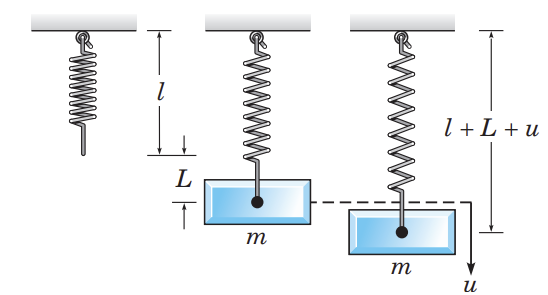
\includegraphics[width=12cm]{DE-ch3-3.6.png}
\end{figure}
Consider an object with mass $m$, and hence weight $W=mg$, hanging on a spring with original length $l$. Due to the application of the mass, the spring elongates to a length $l + L$; by Hooke's law, we know that when the extension $L$ is suitably small (within the limit of proportionality), the spring experiences a restoring force $F_s = -kL$ in the opposite direction to the mass's weight, where $k$ is the constant of proportionality of the spring. When the spring is in equilibrium, the net force is zero and thus we have
\begin{equation*}
    mg = kL.
\end{equation*}
How does the system reach such an equilibrium? To answer this, we must study the displacement of the mass at time $t$ from this initial position, where the spring's extension is $L$. Call this displacement $u(t)$, or simply $u$, measured positively downwards from $l+L$. Thus, as shown in the figure, the length of the spring at any time is given by $l + L + u$, and hence the restoring force is given by 
\begin{equation*}
    F_s(t) = -k(L+u(t))
\end{equation*}
This equation is always true even if $L+u$ is negative (the spring is compressed), as in that case the restoring force would be positive. The mass will always apply a constant weight $W=mg$ downward. We must also take into account the existence of a resistive force on the mass, due to either air resistance (or resistance from other mediums), energy dissipation, friction, or some other source. We assume that this resistive force is proportional to the speed $u'(t)$ of the mass, and directed upward:
\begin{equation*}
    F_d(t) = -\gamma u'(t)
\end{equation*}
where $\gamma > 0$ is the \it damping constant\normalfont. This equation demonstrates that no matter the direction of the motion of the mass, the resistive force is always in an opposite direction. Finally, there may be an external force applied to the mass that varies with time; this may be because the spring is moving, or because of some periodic source that forces the mass to move. We call this force $F(t)$. \\ \\
To summarize, our system involves the following forces:
\begin{enumerate}
    \item A constant weight $W=mg$, directed downward.
    \item A restoring force $F_s(t) = -k(L+u(t))$, originating from the tension in the spring and directed in the opposite direction to its displacement.
    \item A resistive force $F_d(t) = -\gamma u'(t)$, opposite in direction to the mass's motion. Note that this simple model is not always accurate and can be questioned.
    \item A variable external force $F(t)$.
\end{enumerate}
By Newton's Second Law, we have:
\begin{equation*}
    F_{net} = ma(t) = mu''(t)
\end{equation*}
with $F_{net}$ being given by
\begin{equation*}
    F_{net} = mg + F_s(t) + F_d(t) + F(t) = mg - k(L+u(t)) - \gamma u'(t) + F(t)
\end{equation*}
finally yielding the inhomogeneous constant-coefficient second-order differential equation
\begin{equation*}
    mu''(t) + \gamma u'(t) + ku(t) = F(t)
\end{equation*}
Note that this equation makes several simplifying assumptions, namely that it assumes the restoring force is always under the limit of proportionality, that the resistive force is proportional to speed, and that the weight of the spring itself is negligible. \\ \\
With the initial conditions $u(0) = u_0, u'(0) = v_0$ (initial position and velocity), this becomes a complete initial-value problem with unique solutions (unless, of course, the mass quantum-tunnels into a probabilistic cloud during its course of motion and now has seventy different potential values for $u$, all of them being simultaneously correct). Let's consider a few applications of this in practice.
\subsubsection{Undamped free vibrations} \normalfont "Free" vibrations are ones where the external force $F(t)$ is zero (as opposed to "forced" vibrations, which are forced to happen by the external force). If we suppose that there is no damping, then the damping constant $\gamma$ is zero as well. This gives us the equation
\begin{equation*}
    mu''(t)+ku(t) = 0
\end{equation*}
which gives solutions
\begin{equation*}
    u = A\cos \omega_0 t + B\sin \omega_0 t
\end{equation*}
where $\omega_0^2 = \frac{k}{m}$. We can conveniently rewrite this in the form $u = R\cos(\omega_0 t - \delta) = R(\cos\delta \cos \omega_0 t + \sin \delta \sin \omega_0 t)$, as comparing coefficients obtains
\begin{equation*}
    \begin{cases}
        A = R\cos \delta, B = R\sin\delta \\
        R^2 = A^2 + B^2, \frac{B}{A} = \tan \delta
    \end{cases}
\end{equation*}
From $u = R\cos(\omega_0 t - \delta)$ we observe that the \it amplitude \normalfont of the vibrations is $R$, the \it period \normalfont is $\frac{2\pi}{\omega_0}$, the \it phase \normalfont is $\delta$ (displaced $\delta$ radians rightward from normal), and the \it natural frequency \normalfont is $\omega_0$. If no external force is applied, the system will continue oscillating without stopping, and will always vibrate at frequency $\omega_0$ regardless of initial conditions (though the amplitude will be affected). The period is proportional to $\sqrt{m}$ and inversely proportional to $\sqrt{k}$, so larger masses vibrate more slowly and stiffer springs vibrate faster. \\ \\
\subsubsection{Damped free vibrations} \normalfont In this case, the external force $F(t)$ remains zero but the damping coefficient $\gamma > 0$. Our equation is 
\begin{equation*}
    mu''(t) + \gamma u'(t) + ku(t) = 0
\end{equation*}
with characteristic equation
\begin{equation*}
    m\lambda^2 + \gamma \lambda + k = 0
\end{equation*}
yielding solutions
\begin{equation*}
    \lambda_{1, 2} = \frac{-\gamma \pm \sqrt{\gamma^2 - 4km}}{2m}
\end{equation*}
Thus, we will examine a few cases based on the value of $\gamma$.
\begin{enumerate}
    \item \bf $\gamma < \sqrt{4km}$. \normalfont This is known as \it underdamping\normalfont; the damping coefficient is very small, and the resistive force will also be fairly small in this case. As such, the solutions for $\lambda$ are complex with negative real part ($\gamma > 0$). We thus have 
    \begin{equation*}
        u(t) = e^{-\frac{\gamma}{2m}t}(A\cos \mu t + B\cos \mu t), \mu = \frac{\sqrt{4km-\lambda^2}}{2m}
    \end{equation*}
    \begin{figure}[h]
        \centering
        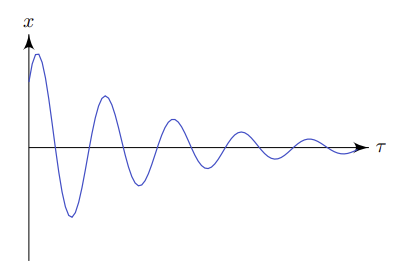
\includegraphics[width=8cm]{DE-ch3-underdamping.png}
    \end{figure} 
    \item $\lambda = \sqrt{4km}$. This is the \it critical damping \normalfont case, where the damping given ensures that the system returns to equilibrium in the shortest time. In this case, we write
    \begin{equation*}
        u(t) = (At+B)e^{-\frac{\gamma}{2m}t}
    \end{equation*}
    \begin{figure}[h]
        \centering
        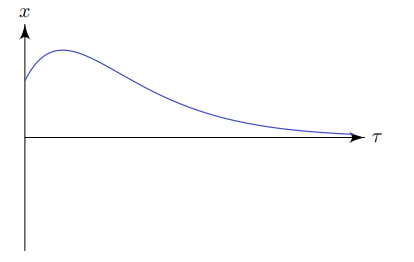
\includegraphics[width=8cm]{DE-ch3-criticaldamping.png}
    \end{figure} 
    \item $\lambda > \sqrt{4km}$. This is the \it overdamping \normalfont case, where the damping force is too large and the system returns to equilibrium slower than if critically damped. The equation gives
    \begin{equation*}
        u(t) = Ae^{\lambda_1 t} + Be^{\lambda_2 t}.
    \end{equation*}
    \newpage
    \begin{figure}[h]
        \centering
        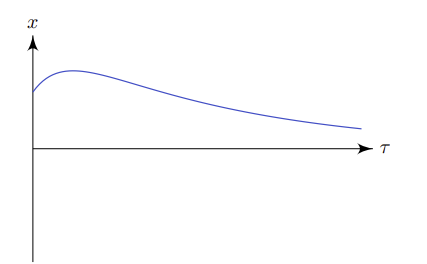
\includegraphics[width=7cm]{DE-ch3-overdamping.png}
    \end{figure} 
\end{enumerate}
(Images courtesy of Dexter Chua. Thanks!) \\ \\
These three cases each yield different forms of solutions for $u(t)$, and each correspond to a different physical scenario. It is very important to note that in every case, the value of $u(t)$ decays to 0 as $t \to \infty$; this confirms our expectations that damping (resistive forces) would lead to the system gradually being pushed back to equilibrium. \\ \\
In the latter two cases (critical and over-damping), no oscillations occur; in the underdamping case, however, the system does begin oscillating (though at a decreasing amplitude). Similar to the undamped case, we can rewrite $u(t)$ for underdamping as 
\begin{equation*}
    u(t)=e^{-\frac{\gamma}{2m}t}(A\cos\mu t + B\sin\mu t) = Re^{-\frac{\gamma}{2m}t}\cos(\mu t - \delta)
\end{equation*}
for certain $R$ and $\delta$, with $\mu = \frac{\sqrt{4km-\gamma^2}}{2m}$ being referred to as the \it quasi-frequency\normalfont. Analogously, $\frac{2\pi}{\mu}$ is the \it quasi-period.\normalfont \\ \\
To examine the effect of underdamping on the system, let us compare the quasi-frequency to the undamped frequency $\omega_0 = \sqrt{\frac{k}{m}}$. We find that 
\begin{equation*}
    \frac{\mu}{\omega_0} = \frac{\sqrt{4km-\gamma^2}}{\sqrt{4km}} = \sqrt{1-\frac{\gamma^2}{4km}} \approx 1-\frac{\gamma^2}{8km}
\end{equation*}
where the final approximation is due to the binomial expansion, when $\gamma$ is very small. Thus, the effect of underdamping is to slightly reduce the frequency of the system (and slightly increase the period). As $\frac{\gamma^2}{4km}$ gradually approaches 0, the frequency approaches 0, transforming the system into one that is critically damped.\\ \\
\subsubsection{Forced vibrations} \normalfont Forced vibrations occur when the external force $F(t)$ is nonzero, producing an inhomogeneous second-order DE. Usually, this force will be an oscillating force of the form $F(t) = F_0 \cos \omega t$ where $F_0$ and $\omega$ represent the amplitude and frequency, respectively. This results in the following differential equation:
\begin{equation*}
    mu''(t) + \gamma u'(t) + ku(t) = F_0 \cos \omega t
\end{equation*}
which, assuming that the solution of the inhomogeneous equation is $u = c_1u_1 + c_2u_2$, yields the solution
\begin{equation*}
    u(t) = c_1u_1 + c_2u_2 + A\cos\omega t + B\sin\omega t
\end{equation*}
for some constants $A$, $B$. As shown in the above section, $c_1u_1 + c_2u_2$ decays to 0 as $t \to \infty$; thus, we refer to $u_c(t) = c_1u_1 + c_2u_2$ as the \it transient solution. \normalfont As $t$ grows larger, it will eventually become negligible in magnitude compared to $U(t) = A \cos \omega t + B\sin \omega t$, which persists indefinitely and is referred to as the \it steady-state solution \normalfont or the \it forced response\normalfont.
\begin{figure}[h]
    \centering
    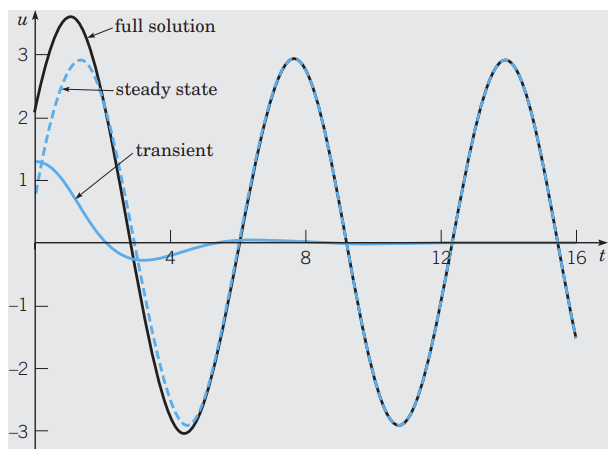
\includegraphics[width=10cm]{DE-ch3-transient.png}
\end{figure} \\
The transient part of the solution allows for any initial conditions to be satisfied. However, it vanishes very quickly compared to the steady-state solution.
\subsubsection{Resonance}
If our steady-state solution is rewritten algebraically as 
\begin{equation*}
    U(t) = R\cos (\omega t - \delta)
\end{equation*}
we are able to observe that its amplitude $R = \sqrt{A^2 + B^2}$ is dependent directly on $A$ and $B$, and thus dependent on the value of $F_0$. Through algebraic manipulation it is possible to show that:
\begin{equation*}
    \begin{cases}
        R = \frac{F_0}{\Delta} \\
        \Delta = \sqrt{m^2(\omega_0^2 -\omega^2)^2 + \gamma^2\omega^2} \\
        \omega_0^2 = \frac{k}{m}
    \end{cases}
\end{equation*}
with $\omega_0$ referring to the system's natural frequency. We observe that when $\omega \to 0$, $R \approx \frac{F_0}{m\omega_0^2} = \frac{F_0}{k}$; and when $\omega \to \inf$, $R \approx 0$. Between those two extremes, there may be a value of $\omega$ that yields a maximum value of $R$; differentiation reveals that such a value $\omega_{max}$ lies at 
\begin{equation*}
    \omega_{max}^2 = \omega_0^2(1-\frac{\gamma^2}{2mk})
\end{equation*}
which only exists if $\frac{\gamma^2}{2mk} < 1$; otherwise, $R$ is monotonously decreasing. We observe that when $\gamma$ is small, $\omega_{max}$ is very close to $\omega_0$, the natural frequency. This phenomenon is known as \bf resonance\normalfont: at or near the natural frequency, the amplitude of the oscillations reaches a peak. This can have both positive and negative consequences, such as amplifying vibrations produced by vehicles across bridges and potentially causing a collapse.
\begin{figure}[h]
    \centering
    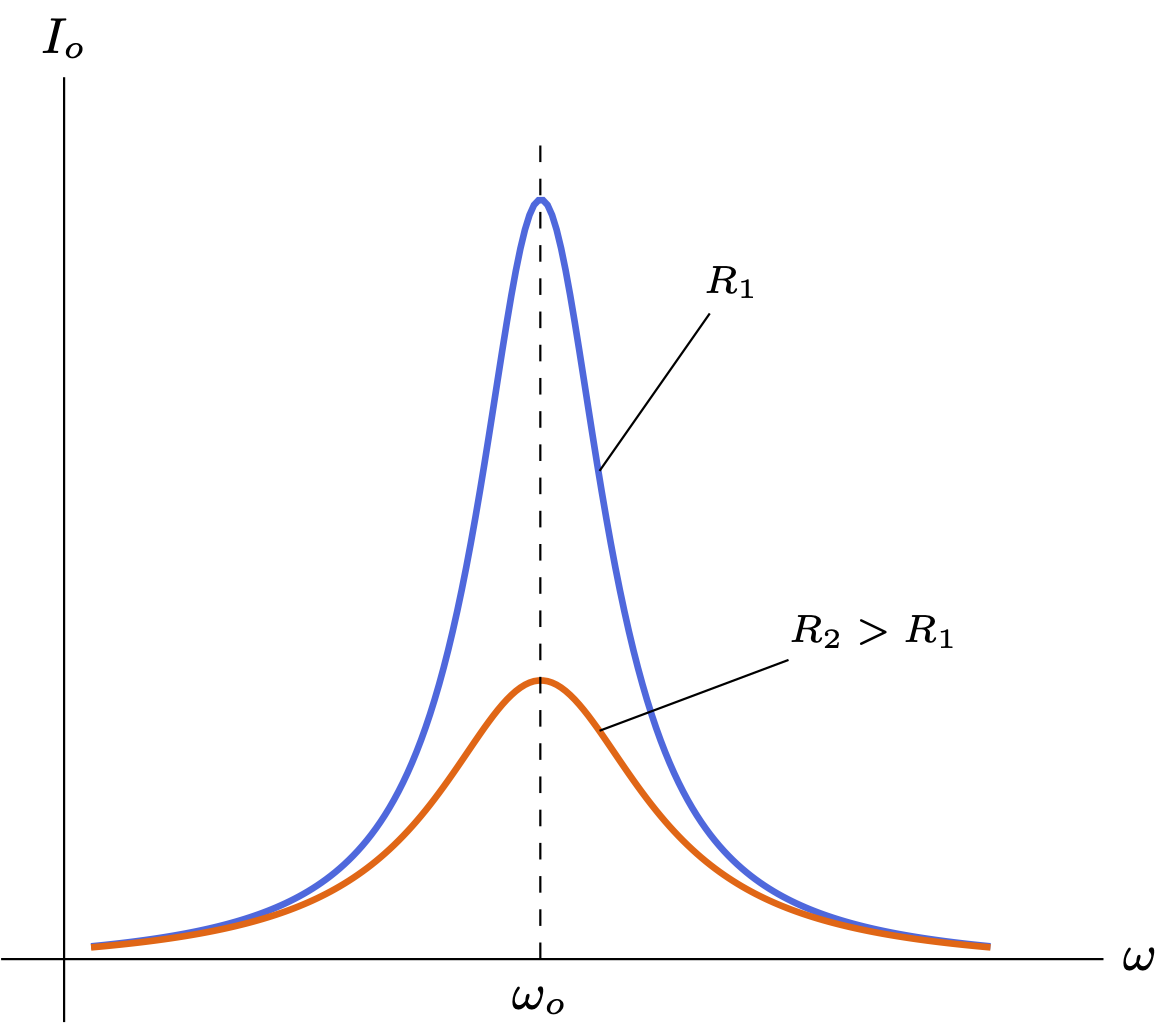
\includegraphics[width=10cm]{DE-ch3-resonance.png}
\end{figure}
\subsection{Impulse functions}
The last section was concerned with the existence of a persistent and periodic external force; however, in many cases, the forces that act on a system are not periodic, but \it impulsive \normalfont- a force of large magnitude that acts only over a short time interval. In other words, this section is concerned with systems modeled by differential equations of type
\begin{equation*}
    au'' + bu' + cu = g(t)
\end{equation*}
where $g(t)$ is large in a specific interval $t_0 - \tau < t_0 < t_0 + \tau$, but zero anywhere else. We define the integral
\begin{equation*}
    I(t) = \int_{t_0-\tau}^{t_0+\tau} g(t)\ dt
\end{equation*}
as the \it impulse \normalfont of the force $g(t)$, a total measure of its strength; or, as $g(t)$ is zero everywhere outside of the interval, we can equivalently write
\begin{equation*}
    I(t) = \int_{-\infty}^{\infty} g(t)\ dt
\end{equation*}
As an example of this, let us consider the following piecewise (discontinuous) function $g(t)$:
\begin{equation*}
    g(t) = \begin{cases}
        \frac{1}{2\tau},\ -\tau < t < \tau\\
        0\ \text{otherwise}
    \end{cases}
\end{equation*}
where it follows that $I(t)$ is always equal to 1, as is verifiable by simple integration. In an ideally impulsive scenario - that is, when this force is as impulsive as possible - the force will act over an infinitesimally small time period; that is, we want $\tau \to 0$, at which point $\lim_{\tau \to 0}I(t)$ is still 1. At this limit, the impulsive force is instantaneous; in physical terms, this can mean that for a ball bouncing on the ground, the duration of its contact with the ground is negligible. A figure of this limiting procedure is shown below:
\begin{figure}[h]
    \centering
    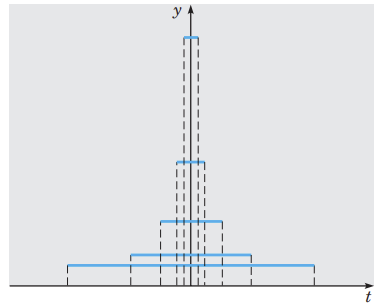
\includegraphics[width=8cm]{DE-ch3-diracdelta.png}
\end{figure}
Hence, we define the limit as $\tau \to 0$ of $g(t)$ to be 
\begin{definition}
    (Dirac delta function). We define the idealized \bf unit impulse function, \normalfont or the \bf Dirac delta function $\delta(t)$\normalfont , as the function which satisfies:
    \begin{equation*}
        \begin{cases}
            \delta(t) = 0, t \neq 0 \\
            \int_{-\infty}^{\infty} \delta(t)\ dt = 1
        \end{cases}
    \end{equation*}
    This represents a function that is only equal to 1 at a discontinuity at $t = 0$; it must be noted that this is not a "function" in the usual sense, as it is zero everywhere except for one point, where it is essentially infinite. It follows from this definition that 
    \begin{equation*}
        \delta(t-t_0) = 0,\ t \neq t_0
    \end{equation*}
    where $\delta(t-t_0)$ can be used to represent a unit impulse at time $t_0$.
\end{definition}
\newpage
\begin{theorem}
    (Integrals involving delta functions). For any function $g(x)$ continuous at $c$, we have
    \begin{equation*}
        \int_{-\infty}^{\infty}g(x)\delta(x-c)\ dx = g(c)
    \end{equation*}
\end{theorem}
\begin{proof}
    First, by the definition of the delta function, we know that outside the specific interval $(c - \tau, c + \tau)$ as $\tau \to 0$, the function is zero:
    \begin{equation*}
        \int_{-\infty}^{\infty}g(x)\delta(x-c)\ dx = \lim_{\tau \to 0} \int_{c-\tau}^{c+\tau} g(x)\delta(x-c)\ dx
    \end{equation*}
    as everywhere else the delta function is zero, resulting in the integral being zero as well. By the Mean Value Theorem, we know that in the interval $(c-\tau, c+\tau)$ there is a value $k$ such that 
    \begin{equation*}
        g(k) = \frac{\int_{c-\tau}^{c+\tau} g(x)\delta(x-c)\ dx}{(c+\tau)-(c-\tau)} = \frac{\int_{c-\tau}^{c+\tau} g(x)\frac{1}{2\tau}\ dx}{(c+\tau)-(c-\tau)}
    \end{equation*}
    by definition of $\delta$. The $\tau$ terms cancel and we are left with
    \begin{equation*}
        g(k) =\int_{c-\tau}^{c+\tau} g(x)\delta(x-c)\ dx
    \end{equation*}
    However, as $\tau \to 0$, the interval becomes infinitely small and only contains the value $x = c$. As such, $c = k$ and the theorem is proven.
\end{proof}
Let's see an example of the Dirac delta function in action for impulse problems. Consider a block of mass 1 kg applied to a spring with spring constant $k = 1$. Assume that there is no damping in this scenario, and set the initial conditions $u = 0$ at $t= 0$ and $t=\pi$. At $t = \frac{\pi}{2}$, there is an instantaneous impulsive force applied to the system, modeled by the delta function $\delta(t-1)$. Thus, we have:
\begin{equation*}
    u'' + u = \delta(t-\frac{\pi}{2})
\end{equation*}
The homogeneous equation has solutions
\begin{equation*}
   u =  A\sin t + B \cos t
\end{equation*}
The initial conditions $u=0,\ t=0$ gives $B = 0$. To deal with the inhomogeneous part (the delta function), we utilize the delta function's piecewise definition and consider the intervals $t < \frac{\pi}{2}$, $t = \frac{\pi}{2}$ and $t > \frac{\pi}{2}$. We assume that $u$ is continuous (both because this is a physical system where discontinuities would not make sense, and because it simplifies the calculations). When $t < \frac{\pi}{2}$, $\delta(t-\frac{\pi}{2}) = 0$; thus the full solution is the same as the complementary function. When $t = \frac{\pi}{2}$, the delta function is infinite (and discontinuous), so we will have to use its limit definition inside an integral. First, we integrate both sides from $\frac{\pi}{2}^-$ to $\frac{\pi}{2}^+$:
\begin{equation*}
    \int_{\frac{\pi}{2}^-}^{\frac{\pi}{2}^+} u'' \ dt + \int_{\frac{\pi}{2}^-}^{\frac{\pi}{2}^+} u \ dt = \int_{\frac{\pi}{2}^-}^{\frac{\pi}{2}^+} \delta(t-\frac{\pi}{2})\ dt
\end{equation*}
As $u$ is continuous, the integral of $u$ at a single point is zero; the right-hand side equals 1 by definition. Thus we have
\begin{equation*}
    [u']^{\frac{\pi}{2}^+}_{\frac{\pi}{2}^-} = 1 = A\sin\frac{\pi}{2} + B\cos\frac{\pi}{2} = A
\end{equation*}
so $A = 1$. 
\subsubsection*{Heaviside step function}
\begin{definition}
    We define $H(x)$, the Heaviside step function, as 
    \begin{equation*}
        H(x) = \int_{-\infty}^{x} \delta(t)\ dt.
    \end{equation*}
    Thus, we have
    \begin{equation*}
        H(x)=\begin{cases}
            0,\ x<0 \\
            1,\ x>0 \\
            \text{undefined, }x=0
        \end{cases}
    \end{equation*}
    with $\frac{dH}{dx} = \delta(x)$ by the Fundamental Theorem of Calculus. These relationships can only be used inside of integrals. \\ \\
    The Heaviside step function is useful in modeling many physical scenarios, namely systems like switches of an electronic circuit which can be turned on and off indefinitely.
\end{definition}

\subsection{Example sheet problems}
\subsubsection*{Find the general solutions of:
\begin{enumerate}
    \item $y'' + 5y'+6y=e^{3x}$,
    \item $y''+9y=\cos 3x$,
    \item $y''+2y'+5y=0$,
    \item $y''-2y'+y=(x-1)e^x$.
\end{enumerate}}
\sout{If I have to type the words "\bf Solution: \normalfont solve characteristic equation, guess functions, suffer a minor mental breakdown etc. etc." again, I think I'm going to have thirteen different aneurysms at the same time.} So I hope you'll excuse my (entirely justified, morally correct, net positive for human society as a whole) laziness here! \\ \\
Except for the first, each of the above four equations all have some sort of hiccup that make them consume one more braincell to compute than your average cookie-cutter DE. \\ \\
The first one proceeds as standard; the characteristic equation yields $\lambda = -2, -3$, and the right-hand side (inhomogeneous term) does not coincide with the complementary function, so the particular integral can be found by guessing functions of the form $Ae^{3x}$. We obtain the general solution $y=Ae^{-3x}+Be^{-2x}+\frac{e^{3x}}{20}$. \\ \\
The second equation is a bit more involved. The complementary function can be found to be $A\sin 3x + B\cos 3x$, and the inhomogeneous term is part of this complementary function. Guessing $x(A\sin 3x + B\cos 3x)$ resolves the issue, yielding the solution $y=A\sin 3x + B\cos 3x + \frac{1}{6}x\sin 3x$. \\ \\
The third equation contains a hiccup roughly the size of a single bubble of carbon dioxide evaporating off the surface of an opened bottle of Diet Coke that's been hanging out in the sun for longer than Margaret Thatcher's grave. We have two complex roots here ($\lambda = -1 \pm i$), so simply $y=e^{-x}(A\sin x + B\cos x)$ works. \\ \\
Finally, the fourth equation requires some care. The homogeneous equation is in the repeated root case, yielding a complementary function $e^x(Ax+B)$. But lo and behold, this means that both $xe^x$ and $e^x$ (the right-hand side term) are in the complementary function already. Jiminy cricket! This means we'll have to move on to terms of order $x^2 e^x$ and $x^3 e^x$ (there are two terms in the forcing term, so we have to use the next two orders); thankfully, this works out for us, yielding the full solution $y=(Ax+B)e^x + \frac{x^3e^x}{6} - \frac{x^2 e^x}{2}$.

\hrulefill
\subsubsection*{The function $y(x)$ satisfies the linear equation
\begin{equation*}
    y''+p(x)y'+q(x)y=0.
\end{equation*}
Let $y_1(x)$ and $y_2(x)$ denote two independent solutions to this equation. Use the Wronskian
\begin{equation*}
    W(x) = \begin{vmatrix}
        y_1 & y_2 \\
        y_1' & y_2'
    \end{vmatrix}
\end{equation*}
to determine a first-order inhomogeneous differential equation for $y_2(x)$. Hence, show that 
\begin{equation*}
    y_2(x) = y_1(x)\int_{x_0}^{x} \frac{W(t)}{y_1(t)^2}\ dt.
\end{equation*}
Show that $W(x)$ satisfies
\begin{equation*}
    \frac{dW}{dx} + p(x)W = 0.
\end{equation*}
Verify that $y_1(x)=1-x$ is a solution of 
\begin{equation*}
    xy'' - (1-x^2)y' - (1+x)y = 0.
\end{equation*}
Hence, using the above with $x_0 = 0$ and expanding the integrand in powers of $t$ to order $t^3$, find the first three non-zero terms in the power series expansion for a solution, $y_2$, of the differential equation that is independent of $y_1$ and satisfies $y_2(0)=0, y_2''(0)=1$.
}
\bf Solution. \normalfont Using the definition of the Wronskian, we have
\begin{equation*}
    W(x) = y_1 y_2' - y_1' y_2
\end{equation*}
Reorganizing this as a differential equation in $y_2$ and noting that $W$, $y_1$ are presumed to be known, we have $y_2' - \frac{y_1'}{y_1} y_2 = \frac{W(x)}{y_1}$. The method of integrating factors with integrating factor
\begin{equation*}
    \mu = e^{\int -\frac{y_1'}{y_1}\ dx} = e^{- \ln y_1} = -\frac{1}{y_1}
\end{equation*}
Multiplying throughout gives 
\begin{equation*}
    -(\frac{y_2}{y_1})' = -\frac{W(x)}{y_1}
\end{equation*}
and thus 
\begin{equation*}
    y_2 = y_1 \int \frac{W(x)}{y_1^2} \ dx = y_1 \int_{x_0}^x \frac{W(t)}{y_1(t)^2}\ dt
\end{equation*}
where $x_0$ accounts for the constant in the indefinite integral, as desired. \\ \\
The next part requires us to show that $W(x)$ satisfies $\frac{dW}{dx} + p(x)W = 0$; plugging in $W(x) = y_1y_2'-y_1'y_2$ obtains the desired result (exact derivation found in proof for Abel's theorem above). \\ \\
Now, we consider the differential equation 
\begin{equation*}
    xy''-(1-x^2)y'-(1+x)y=0.
\end{equation*}
The function $y_1(x) = 1-x$ has $y_1' = -1, y_1'' = 0$; plugging this in results in $x(0) - (1-x^2)(-1) - (1+x)(1-x) = (1-x^2)-(1-x^2)  = 0$. To find the second independent solution $y_2$, we will attempt to emulate the method given to us above. To produce an equation of the form
\begin{equation*}
    y''+p(x)y'+q(x)y=0
\end{equation*}
with leading coefficient 1, as given above, we divide throughout by $x$:
\begin{equation*}
    y'' + \frac{x^2-1}{x} - \frac{1+x}{x}y = 0
\end{equation*}
The Wronskian for this equation is given by 
\begin{equation*}
    \frac{dW}{dx} + p(x)W = \frac{dW}{dx} + \frac{x^2-1}{x}W = 0 
\end{equation*}
and thus 
\begin{equation*}
    \begin{aligned}
    \int \frac{dW}{W} &= \int \frac{1-x^2}{x}\ dx \\
    \ln W &= \int \frac{1}{x} - x \ dx \\
    \ln W &= \ln x - \frac{x^2}{2} + C \\
    W &= Axe^{-\frac{x^2}{2}}
    \end{aligned}
\end{equation*}
for an arbitrary constant $A$. Next, using the formula for $y_2$ derived above, with $y_1(x) = 1-x$, $x_0=0$, and $W = Axe^{-\frac{x^2}{2}}$:
\begin{equation*}
    y_2(x)=y_1(x)\int^{x}_{0} \frac{W(t)}{y_1(t)^2}\ dt = A(1-x)\int^{x}_{0} \frac{te^{-\frac{t^2}{2}}}{(1-t)^2} \ dt
\end{equation*}
This obviously seems non-integrable (although I dare you to prove me wrong), and so we use the power series expansion for $e^{\frac{-x^2}{2}}$:
\begin{equation*}
    e^{-\frac{x^2}{2}} = 1 + \frac{(-\frac{x^2}{2})}{1!} + \frac{(-\frac{x^2}{2})^2}{2!} + \dots
\end{equation*}
where we only need the first two terms $1-\frac{x^2}{2}$ because the question asks for terms up to the order $x^3$. We also have to deal with the presence of $(1-t)^{-2}$, which by the binomial expansion yields
\begin{equation*}
    1+2t+3t^2+\dots
\end{equation*}
Where we take only the first three terms. Returning to our integral, we have
\begin{equation*}
    y_2=A(1-x)\int^{x}_{0} te^{-\frac{t^2}{2}}(1-t)^{-2}\ dt = A(1-x)\int^{x}_{0} t(1-\frac{t^2}{2})(1+2t+3t^2) \ dt
\end{equation*}
To the order of the $t^3$ term in the integrand, this is
\begin{equation*}
    A(1-x)\int_{0}^{x}t + 2t^2 + \frac{5t^3}{2} \ dt = A(1-x)(\frac{x^2}{2}+\frac{2}{3}x^3+\frac{5}{8}x^4)
\end{equation*}
which expands to
\begin{equation*}
    A(\frac{x^2}{2} + \frac{x^3}{6} -\frac{x^4}{24})
\end{equation*}
for the first three terms. If we want $y_2(0) = 0, y_2''(0) = 1$, then:
\begin{equation*}
    y_2'' = A(1+x-\frac{x^2}{2}),\ y_2''(0) = A
\end{equation*}
and so $A=1$. Thus, our solution is $y_2(x) = \frac{x^2}{2} +\frac{x^3}{6}-\frac{x^4}{24}$.
 
\hrulefill
\subsubsection*{Find the general solutions of:
\begin{enumerate}
    \item $y_{n+2}+y_{n+1}-6y_n = n^2$,
    \item $y_{n+2}-3y_{n+1}+2y_n = n$,
    \item $y_{n+2}-4y_{n+1}+4y_n = a^n$, $a$ real.
\end{enumerate}}
\bf Solution. \normalfont The above three equations are difference equations of order 2 with constant coefficients. \\ \\
The first two equations require nothing beyond finding roots to the characteristic equation, writing out the complementary function, then guessing a polynomial of degree 2 and 1 respectively. This method yields
\begin{equation*}
    y_n = A((-3)^n) + B(2^n) -\frac{n^2}{4}-\frac{3n}{8}-\frac{19}{32}
\end{equation*}
for (1), and 
\begin{equation*}
    y_n = A(2^n)+B-\frac{n(n+1)}{2}-1
\end{equation*}
for (2), which requires a particular integral of degree 2 because its coefficients sum to 0 (cancelling the $n$ term for a PI of degree 1). \\ \\
Finally, the third equation requires closer examination. The homogeneous equation can be easily solved as $(A+Bn)2^n$ (the repeated root case); in normal circumstances, we would simply guess $ka^n$ as the particular integral and be on our merry way:
\begin{equation*}
    \begin{aligned}
        y_n &= ka^n \ \text{for some $k$} \\
        y_{n+2}-4y_{n+1}+4y_n &= ka^2 a^n - 4ka(a^n)+4ka^n = a^n\\
        &=(ka^2-4ka+4k)a^n \\
        k(a-2)^2 &= 1 \\
        k &= \frac{1}{(a-2)^2}
    \end{aligned}
\end{equation*}
Quick sanity checks can confirm that this equation works for any value of $a \neq 2$. However, what happens when $a=2$? In that case, the particular integral would be part of the solution to the homogeneous equation and the expression above would not be valid (as expressed by the fact that $a=2$ is an asymptote). We also observe that $n2^n$ is part of the homogenous solution. To circumvent this, we guess the next-lowest ordered term, $An^2 2^n$, as a particular integral instead:
\begin{equation*}
    \begin{aligned}
        y_n &= An^2 2^n \text{ for some $A$} \\
        y_{n+2}-4y_{n+1}+4y_n &= 4A(n^2+4n+4)2^n - 8A(n^2+2n+1)2^n + 4An^2 2^n = 2^n \\
        &=(8A)2^n \\
    \end{aligned}
\end{equation*} 
yielding $A=\frac{1}{8}$ and the full solution
\begin{equation*}
    y_n = (An+B)2^n + \frac{1}{8}n^2 2^n.
\end{equation*}

\hrulefill

\subsubsection*{(i) Find the solution of $y''-y'-2y=0$ that satisfies $y(0) = 1$ and is bounded as $x \to \infty$. \\ \\
(ii) Solve the related difference equation 
\begin{equation*}
    (y_{n+1}-2y_n + y_{n-1}) - \frac{1}{2}h(y_{n+1}-y_{n-1}) - 2h^2 y_n = 0,
\end{equation*}
and show that if $0 < h << 1$ the solution that satisfies $y_0 = 1$ and for which $y_n$ is bounded as $n \to \infty$ is approximately $y_n = (1-h+\frac{1}{2}h^2)^n$. Explain the relation with the solution of (i).}
\bf (i) Solution. \normalfont Proceeding normally with the characteristic equation yields simply
\begin{equation*}
    y = Ae^{-x}+Be^{2x}
\end{equation*}
for constants $A$, $B$. To satisfy the boundary conditions we must have
\begin{equation*}
    \begin{cases}
        y(0) = Ae^0 + Be^0 = A + B = 1 \\
        \lim_{x\to \infty} Ae^{-x} + Be^{2x} = 0 + \lim Be^{2x} \text{ is bounded} \iff B = 0 \\
    \end{cases}
\end{equation*}
and thus $A = 1$, yielding
\begin{equation*}
    y =e^{-2x}.
\end{equation*}
\bf (ii) Solution. \normalfont We aggressively ignore any intelligent hints our pattern-seeking brain is giving us about any devious links between the difference equation and the differential equation for now, and charge forward towards solving the difference equation like a caveman throwing rocks at a bear. Reorganizing the equation gives
\begin{equation*}
    (1-\frac{h}{2})y_{n+1} - (2+2h^2)y_n + (1+\frac{h}{2})y_{n-1} = 0
\end{equation*}
which, by the method of characteristic equations, yields roots
\begin{equation*}
    \begin{aligned}
    \lambda_1, \lambda_2 &= \frac{2+2h^2\pm \sqrt{4+4h^4+8h^2-4(1-\frac{h}{2})(1+\frac{h}{2})}}{2(1-\frac{h}{2})} \\
    &= \frac{2+2h^2\pm h\sqrt{4h^2+9}}{2-h}
    \end{aligned}
\end{equation*}
Note that the discriminant is necessarily positive, yielding solutions of the form $y_n = A(\lambda_1)^n + B(\lambda_2)^n$. When $h$ is infinitesimally small, we can write:
\begin{equation*}
    \lambda_{1, 2} \approx \frac{2 +2h^2 \pm h\sqrt{9 + 4(0)^2}}{2(1-\frac{1}{2}h)} = (1\pm \frac{3}{2}h+h^2)(1-(\frac{1}{2}h))^{-1}
\end{equation*}
Thus we write the full solution as
\begin{equation*}
   y_n= A((1+ \frac{3}{2}h+h^2)(1-\frac{1}{2}h)^{-1})^n + B((1 - \frac{3}{2}h+h^2)(1-\frac{1}{2}h)^{-1})^n
\end{equation*}
As $y_n$ needs to be bounded as $n \to \infty$ (per the problem's restrictions), we recognize that the first term is a power of something greater than 1 and thus diverges, so we leave only the second term in our full solution. Furthermore, we have the condition $y_0 = 1$, implying $B = 1$. Thus, we write
\begin{equation*}
    y_n \approx ((1-\frac{3}{2} h + h^2)(1-\frac{1}{2}h)^{-1})n
\end{equation*}
To convert this to the desired form, we utilize the binomial expansion of $(1-\frac{1}{2}h)^{-1}$ and calculate up to the term in $h^2$:
\begin{equation*}
    \begin{aligned}
        y_n&=((1-\frac{3}{2}h+h^2)(1+\frac{1}{2}h+\frac{1}{4}h^2+\dots))^n \\
        &=((1 - \frac{3}{2}h + h^2 + \frac{1}{2}h - \frac{3}{4} h^2 + (\text{cubic term}) + \frac{1}{4}h^2))^n \\
        &=(1-h+\frac{h^2}{2})^n
    \end{aligned}
\end{equation*}
as desired.
\\ \\
To consider the connection between the two equations in the problem, we have to first ask ourselves: when does the difference equation begin to look like a differential equation? The function in the difference equation $y_n$ takes only discrete values of $n$, that is: 
\begin{equation*}
    y(0), y(1), y(2), \dots
\end{equation*}
But if we lessened the gap between two values - that is, instead of $y(n)$ and $y(n+1)$ we had $y(n)$ and $y(n+h)$ - we would have something that looks much more continuous. Let us consider the sequence
\begin{equation*}
    y_0 = f(0), y_1 = f(h), y_2 = f(2h)\dots
\end{equation*}
We clearly recognize that as $h \to 0$, this sequence is simply the continuous function $f$. This is the fundamental connection between difference equations and differential equations: difference equations are just discretized versions of differential equations. \\ \\
To relate this to the equations in our problem, we consider the discrete concept of a slope and the continuous concept of a derivative. The slope between any two adjacent points $y_n=f(nh)$ and $y_{n+1}=f((n+1)h)$ in a difference equation is 
\begin{equation*}
    \frac{y_{n+1}-y_n}{h}
\end{equation*}
and, equivalently, the gradient between any two adjacent "points" on a continuous function $f(x)$ is simply 
\begin{equation*}
    \frac{df}{dx}(x).
\end{equation*}
When $h$ becomes infinitely small, the first expression approximates the second; we can also write 
\begin{equation*}
    \frac{y_{n+1}-y_{n-1}}{2h} \approx \frac{dy}{dx}
\end{equation*}
as the points are infinitely close to each other. This condition is indeed true in this problem. Similarly, the second derivative is simply the rate of change (gradient) of the first derivative, so its discrete analogue in a difference equation would be 
\begin{equation*}
    \frac{d^2 f}{dx^2} (x) \approx \frac{\frac{y_{n+1}-y_{n}}{h} - \frac{y_{n}-y_{n-1}}{h}}{h} = \frac{y_{n+1}-2y_n +y_{n-1}}{h^2}
\end{equation*}
the slope between the rate of change at $y_n$ and that at $y_{n+1}$, with a distance of $h$ between them. And voila! This matches the form we were given all the way back, when we started the problem but chose to ignore why the difference equation was written in that specific way. From all the way back then, we had:
\begin{equation*}
    (y_{n+1}-2y_n + y_{n-1}) - \frac{1}{2}h(y_{n+1}-y_{n-1}) - 2h^2 y_n = 0,
\end{equation*}
or rather
\begin{equation*}
    \frac{1}{h^2}(y_{n+1}-2y_n + y_{n-1}) - \frac{(y_{n+1}-y_{n-1})}{2h} - 2y_n = 0,
\end{equation*}
which, using the forms given above, is approximately
\begin{equation*}
    y'' - y' -2y
\end{equation*}
when $h$ is very small. This suggests to us that the difference equation given is simply a discrete transformation of the differential equation; it stands to reason, therefore, that the solution of the difference equation is a good approximation to the solution of the differential equation. Is this true? Examining
\begin{equation*}
    y_n = (1-h+\frac{h^2}{2})^n
\end{equation*}
allows us to see that $1-h+\frac{h^2}{2}$ are the first three terms of the Taylor expansion of $e^{-h}$, making the solution an approximation for $e^{-nh}$:
\begin{equation*}
    y_n \approx e^{-nh}
\end{equation*} 
which is the same form to that of the differential equation.

\hrulefill

\subsubsection*{Show that 
\begin{equation*}
    \frac{1}{r^2}\frac{d}{dr}(r^2 \frac{dT}{dr}) = \frac{1}{r}\frac{d^2}{dr^2}(rT)
\end{equation*}
and hence solve the equation
\begin{equation*}
    \frac{1}{r^2}\frac{d}{dr}(r^2\frac{dT}{dr}) = k^2 T
\end{equation*}
subject to the conditions that $T$ is finite at $r=0$ and $T(1) = 1$.}
\bf Solution. \normalfont The first part follows from taking the required derivatives:
\begin{equation*}
    \begin{aligned}
        \frac{1}{r^2}\frac{d}{dr}(r^2\frac{dT}{dr}) &= \frac{1}{r^2}(2r\frac{dT}{dr} + r^2\frac{d^2T}{dr^2}) \\
        &= \frac{1}{r}(2\frac{dT}{dr} + r\frac{d^2T}{dr^2})\\ \\
        \frac{1}{r}\frac{d^2}{dr^2}(rT) &= \frac{1}{r}\frac{d}{dr}(T+r\frac{dT}{dr}) \\
        &= \frac{1}{r}(\frac{dT}{dr}+\frac{dT}{dr}+r\frac{d^2T}{dr^2})
    \end{aligned}
\end{equation*}
as desired.
To solve the equation, we apply the identity shown above on the left-hand side:
\begin{equation*}
    \begin{aligned}
    \frac{1}{r^2}\frac{d}{dr}(r^2\frac{dT}{dr}) &=\frac{1}{r}\frac{d^2}{dr^2}(rT) = k^2 T
    \end{aligned}
\end{equation*}
Consider the substitution $u=rT,\ T=\frac{u}{r}$:
\begin{equation*}
    \frac{1}{r}\frac{d^2u}{dr^2} = \frac{u}{r},\ \frac{d^2u}{dr^2} - u = 0
\end{equation*}
which, by characteristic equations, simply yields $u=rT=Ae^r+Be^{-r}$ for constants $A$ and $B$, and thus:
\begin{equation*}
    T=\frac{Ae^r+Be^{-r}}{r}.
\end{equation*} The only way this can approach a finite limit when $r=0$ is if the numerator is also zero: $Ae^0 + Be^0 = 0$, meaning $A = -B$. Combined with the initial condition $T(1) = 1$, we have
\begin{equation*}
    Ae + \frac{B}{e} = A(e-\frac{1}{e}) = 1, A = \frac{e}{e^2-1}, B = -\frac{e}{e^2-1}.
\end{equation*}

\hrulefill

\subsubsection*{Given the solution $y_1(x)$, find a second solution of the following equations:
\begin{enumerate}
    \item $x(x+1)y'' + (x-1)y' - y = 0,\ y_1(x)=(x+1)^{-1}$;
    \item $xy''-y'-4x^3y=0,\ y_1(x)=e^{x^2}$.
\end{enumerate}
}
\bf Solution. \normalfont We probably know that just tacking on an $x$ to $(x+1)^{-1}$ like I tack terrible jokes onto these lecture notes would give us a solution that works; but, incidentally, writing down "multiply by $x$, because my brain told me so" is also probably the best way to guarantee going home with a brand-new shiny wooden spoon stuck between your teeth. So let's try and prove these solutions rigorously (or as rigorously as we can, seeing as this is a Differential Equations course). \\ \\
Let $y_2(x)$, the other independent solution, be $y_1$ multiplied by any function of $x$: $y_2(x) = v(x)y_1(x)$ (or $vy_1$ if we're being intimate). Thus, we write:
\begin{equation*}
    \begin{aligned}
        y_2'(x) &= (vy_1)' = v'y_1 + vy_1' \\
        y_2''(x) &= (v'y_1+vy_1')' \\
        &= v''y_1 + 2v'y_1' + vy_1''
    \end{aligned}
\end{equation*}
Plugging into the first equation with $y_1=(x+1)^{-1}$ gives:
\begin{equation*}
    \begin{cases}
        y_1' = -(x+1)^{-2}, \ y_1'' = 2(x+1)^{-3} \\
        y_2'(x) = v'y_1 + vy_1' = v'(x+1)^{-1} - v(x+1)^{-2} \\
        y_2''(x) = 2(x+1)^{-3}v - 2(x+1)^{-2}v' + (x+1)^{-1}v''
    \end{cases}
\end{equation*}
Thus, the first DE can be rewritten as 
\begin{equation*}
    xv'' - 2x(x+1)^{-1}v' + 2x(x+1)^{-2}v + (x-1)(x+1)^{-1}v' - (x-1)(x+1)^{-2}v - (x+1)^{-1}v = 0
\end{equation*}
or, once collecting terms, as 
\begin{equation*}
    xv'' + (\frac{x-1}{x+1} - \frac{2x}{x+1})v' +(\frac{2x}{(x+1)^2} - \frac{x-1}{(x+1)^2} - \frac{1}{x+1})v = 0
\end{equation*}
Simplifying yields
\begin{equation*}
    xv'' - v' = 0.
\end{equation*}
Using the substitution $u = v'$ yields $xu'-u=0, \ln x = \ln u, u = v' = Ax$ for some constant $A$; and thus, as $v' = Ax$, we finally have $v = Bx^2$ (any coefficient works). A second independent solution, as defined, is $y_2 = vy_1 = x^2(x+1)^{-1}$.\\ \\
We proceed with the second equation, where $y_1 = e^{x^2},\ y_1' = 2xe^{x^2}, $ and $y_1'' = 2e^{x^2} + 4x^2e^{x^2}$. We can already tell that this is going to be more tedious than being forced to read the Terms of Service, so let's try a different method. It was shown in a previous problem that the Wronskian of DEs of the form $y''+p(x)y'+q(x)y = 0$ satisfied
\begin{equation*}
    \frac{dW}{dx} + p(x)W = 0
\end{equation*}
Reorganizing the second equation into the desired form yields
\begin{equation*}
y'' - \frac{1}{x} y' + 4x^2y = 0
\end{equation*}
and thus
\begin{equation*}
    \frac{dW}{dx} - \frac{1}{x}W = 0
\end{equation*}
giving $W = Ax$ for some constant $A$ and $W = y_1y_2' - y_1'y_2 = e^{x^2}y_2' - 2xe^{x^2}y_2$. Thus, we have the first-degree inhomogenous DE 
\begin{equation*}
    y_2' - 2xy_2 = Axe^{-\frac{x^2}{2}}
\end{equation*}
which, when multiplying by the integrating factor $e^{-x^2}$, gives
\begin{equation*}
    \begin{aligned}
    (e^{-x^2}y_2)' &= Axe^{-\frac{3x^2}{2}} \\
    e^{-x^2}y_2 &= A\int xe^{-\frac{3x^2}{2}}\ dx \\
    &= Be^{-\frac{3x^2}{2}} \\
    y_2 &= Be^{-\frac{x^2}{2}}
\end{aligned}
\end{equation*}
for some constant $B$.

\hrulefill

\subsubsection*{The $n$ functions $y_j(x)$ ($1 \leq j \leq n$) are independent solutions of the equation
\begin{equation*}
    y^{(n)}(x) + p_1(x) y^{(n-1)}(x) + \dots + p_{n-1}(x)y'(x) + p_n(x)y(x) = 0.
\end{equation*}
Let $\mathbf{W}$ be the $n \times n$ matrix whose $i, j$ element $W_{ij}$ is $y_j^{(i-1)}(x)$ (so that $\det \mathbf{W} = \mathcal{W}$, the Wronskian). Find a matrix $\mathbf{A}$, which does not explicitly involve the $y_j$, such that 
\begin{equation*}
    \mathbf{W}' = \mathbf{A}\mathbf{W}
\end{equation*}
where $\mathbf{W}'$ is the matrix whose elements are given by $(\mathbf{W}')_{ij}=(\mathbf{W}_{ij})'$. Using the identity
\begin{equation*}
    (\ln \det \mathbf{W})' = trace(\mathbf{W}' \mathbf{W}^{-1}),
\end{equation*}
express $\mathcal{W}$ in terms of $p_1(x)$.
}
\bf Solution. \normalfont To clarify matters, we first write down what $\mathbf{W}$ and $\mathbf{W}'$ are supposed to look like:
\begin{equation*}
    \mathbf{W} = \begin{bmatrix}
        y_1(x) & y_2(x) & \dots & y_n(x) \\
        y_1'(x) & y_2' (x) & \dots & y_n'(x) \\
        \vdots & \vdots & \vdots & \vdots \\
        y_1^{(n-1)}(x) & y_2^{(n)}(x) & \dots & y_n^{(n-1)}(x)
    \end{bmatrix}
\end{equation*}
and
\begin{equation*}
    \mathbf{W}' = \begin{bmatrix}
        y_1'(x) & y_2'(x) & \dots & y_n'(x) \\
        y_1''(x) & y_2''(x) & \dots & y_n''(x) \\
        \vdots & \vdots & \vdots & \vdots \\
        y_1^{(n)}(x) & y_2^{(n)}(x) & \dots & y_n^{(n)}(x)
    \end{bmatrix}
\end{equation*}
as every term is the derivative of the corresponding term in $\mathbf{W}$. For $\mathbf{W}' = \mathbf{A}\mathbf{W}$, $\mathbf{A}$ also has to be $n \times n$. Consider the elements of $\mathbf{W}'$ one by one. For $(\mathbf{W}')_{11} = y_1'(x)$, we want the product between the first row of $A$ and first column of $W$ to be $y_1'(x)$:
\begin{equation*}
    \begin{aligned}
        y_1'(x) &=
        \begin{bmatrix}
            a_1 &a_2 &\dots &a_n
        \end{bmatrix}
        \begin{bmatrix}
            y_1(x) \\ y_1'(x) \\ \vdots \\ y_1^{(n-1)}(x)
        \end{bmatrix} \\
        &= a_1y_1(x) + a_2y_1'(x) + \dots + a_ny^{(n-1)}(x) \\
        &= y_1'(x)
    \end{aligned}
\end{equation*}
and by observation we see that a possible solution is $a_2 = 1$, all other $a_i = 0$. Thus the first column of $A$ is 
\begin{equation*}
    \begin{bmatrix}
        0 &1 & 0 & 0 & \dots & 0
    \end{bmatrix}.
\end{equation*}
A similar approach gives the second row as 
\begin{equation*}
    \begin{bmatrix}
        0 & 0 & 1 & 0 & \dots & 0
    \end{bmatrix}.
\end{equation*}
and, in general, the $k$th row as all $0$s except a $1$ in column $k+1$. However, we note that this fails in one particular circumstance: for the last row of $\mathbf{W'}$, $y_j^{(n)}(x)$ is not an element in $\mathbf{W}$ (which contains only up to the $(n-1)$th derivative). To generate that last row, we will need some kind of equation relating the first $n-1$ derivatives of $y_j$ to its $(n)$th derivative. Does such an equation exist? It sure does, and it's the differential equation at the beginning of this problem!
\begin{equation*}
    y^{(n)}(x) + p_1(x) y^{(n-1)}(x) + \dots + p_{n-1}(x)y'(x) + p_n(x)y(x) = 0
\end{equation*}
enables us to write 
\begin{equation*}
    y^{(n)}(x) = -\sum_{i=1}^{n}p_i(x)y^{(n-i)}(x)
\end{equation*}
and as such we can write 
\begin{equation*}
    y_j^{n}(x) = \begin{bmatrix}
        -p_n(x) & -p_{n-1}(x) &\dots &-p_1(x)
    \end{bmatrix}
    \begin{bmatrix}
        y_j(x) \\ y_j'(x) \\ \vdots \\ y_j^{(n-1)}(x)
    \end{bmatrix} 
    = \sum_{i=1}^{n}p_i(x)y^{(n-i)}(x)
\end{equation*}
and thus the last row of $\mathbf{A}$ is
\begin{equation*}
    \begin{bmatrix}
        -p_n(x) & -p_{n-1}(x) &\dots &-p_1(x)
    \end{bmatrix}
\end{equation*}
We conclude that $\mathbf{A}$ has the form
\begin{equation*}
    \mathbf{A} =
    \begin{bmatrix}
        0 & 1 & 0 & 0 & \dots & 0 \\
        0 & 0 & 1 & 0 & \dots & 0 \\
        0 & 0 & 0 & 1 & \dots & 0 \\
        \vdots & \vdots & \vdots & \vdots & \vdots & \vdots \\
        0 & 0 & 0 & 0 & \dots & 1 \\
        -p_n(x) & -p_{n-1}(x) & -p_{n-2}(x) & -p_{n-3}(x) &\dots &-p_1(x)
    \end{bmatrix}
\end{equation*}
With $\mathbf{W'} = \mathbf{AW}$ and hence $\mathbf{A} = \mathbf{W'W^{-1}}$. The identity given by the problem concerns precisely this:
\begin{equation*}
    (\ln \det \mathbf{W})' = trace(\mathbf{W}' \mathbf{W}^{-1}),
\end{equation*}
wherein the right-hand side is simply the trace of $A$, or $-p_1(x)$ (a sum of all diagonal elements, which are all 0 except for $-p_1(x)$). Thus, we have:
\begin{equation*}
    \begin{aligned}
        (\ln \det \mathbf{W})' &= trace(\mathbf{A}) = -p_1(x) \\
        \ln \det \mathbf{W} &= -\int p_1(x) \ dx \\
        \det \mathbf{W} &= e^{-\int p_1(x) \ dx }
    \end{aligned}
\end{equation*}
which is our general expression for the Wronskian.

\hrulefill

\subsubsection*{Let $y(x)$ satisfy the inhomogenous equation
\begin{equation*}
    y''-2x^{-1}y'+2x^{-2}y=f(x).
\end{equation*}
Set
\begin{equation*}
    \begin{pmatrix}
        y \\ y'
    \end{pmatrix}
    = 
    u(x)
    \begin{pmatrix}
        y_1 \\ y_1'
    \end{pmatrix}
    +
    v(x)
    \begin{pmatrix}
        y_2 \\ y_2'
    \end{pmatrix},
\end{equation*}
where $y_1(x)$ and $y_2(x)$ are two independent solutions of the above equation when $f(x) = 0$, and $u(x)$ and $v(x)$ are unknown functions. Obtain first-order differential equations for $u$ and $v$, and hence find the most general solution of the above equation in the case $f(x) = x \sin x$. Are the functions $u$ and $v$ completely determined by this procedure?   
}
\bf Solution. \normalfont This question formalizes the variation of parameters method for finding the particular solution of any linear second-order inhomogenous ODE. As stated by the question, we have
\begin{equation*}
        y = u(x)y_1 + v(x)y_2;
\end{equation*}
for unknown functions $u$, $v$. Taking the derivative yields
\begin{equation*}
    y' = u'y_1 + uy_1' + v'y_2 + vy_2'.
\end{equation*}
We would like to avoid $u'$ and $v'$ terms (as they would give us a second-order DE in $u$ and $v$), so as the problem instructs, we impose the condition
\begin{equation*}
    u'y_1 + v'y_2 = 0
\end{equation*}
to allow for
\begin{equation*}
    y' = uy_1'+vy_2'.
\end{equation*}
As such, we can write 
\begin{equation*}
    y'' = (uy_1'+vy_2')' = u'y_1' + uy_1'' + v'y_2' + vy_2''
\end{equation*}
And the original inhomogeneous equation as 
\begin{equation*}
    \begin{aligned}
        y''-2x^{-1}y' + 2x^{-2}y &= f(x) \\
        uy_1'' + u'y_1' + vy_2'' + v'y_2' - 2x^{-1}(uy_1' + vy_2') + 2x^{-2}(uy_1 + vy_2) &= 0 \\
        u(y_1''-2x^{-1}y_1'+2x^{-2}y_1) + v(y_2''-2x^{-1}y_2'+2x^{-2}y_2) + u'y_1' + v'y_2' &= 0
    \end{aligned}
\end{equation*}
and as $y_1$ and $y_2$ satisfy
\begin{equation*}
    y''-2x^{-1}y'+2x^{-2}y = 0
\end{equation*}
the above equation simplies to
\begin{equation*}
    u'y_1' + v'y_2' = 0
\end{equation*}
forming the system of equations in $u'$ and $v'$:
\begin{equation*}
    \begin{cases}
        u'y_1 + v'y_2 = 0 \\
        u'y_1' + v'y_2' = 0
    \end{cases}
\end{equation*}
which can be solved to obtain 
\begin{equation*}
    \begin{cases}
        u(x) = -\int \frac{f(x) y_2}{\det \mathbf{W}}\ dx \\
        v(x) = \int \frac{f(x) y_1}{\det \mathbf{W}}\ dx
    \end{cases}
\end{equation*}
simply through substitution, where $\mathbf{W}$ denotes the Wronskian. \\ \\
Applying this procedure to the equation
\begin{equation*}
    y'' - 2x^{-1}y' + 2x^{-2}y = x \sin x
\end{equation*}
involves beginning with the homogenous equation
\begin{equation*}
    x^2y'' - 2xy' + 2y = 0
\end{equation*}
which is an equidimensional equation with solutions $y_1 = x$, $y_2 = x^2$ (as can be verified), and thus the Wronskian $x(2x) - x^2 = x^2$. Thus, we have (with $f(x) = x \sin x$):
\begin{equation*}
    \begin{cases}
        u(x) = -\int \frac{x^3 \sin x}{x^2}\ dx = -\int x\sin x\ dx = x\cos x - \sin x \\
        v(x) = \int \frac{x^2 \sin x}{x^2}\ dx = -\cos x
    \end{cases}
\end{equation*}
and thus the particular integral
\begin{equation*}
    y = uy_1 + vy_2 = x(x\cos x - \sin x) - x^2\cos x
\end{equation*}
The functions $u$ and $v$ are not completely determined; in fact, it is worth noting that many different particular integrals may exist, but that they always differ from each other by a constant multiple of the homogeneous equation. We only need one of these particular integrals, and imposing $u'y_1 + v'2y_2$ indeed only gives us one, not all, of the possible solutions that satisfy the given DE.

\hrulefill

\subsubsection*{A large oil tanker of mass $W$ floats on a sea of density $\rho$. Suppose the tanker is given a small downward displacement $z$. The upward force is equal to the weight of the water displaced (Archimedes' Principle). If the cross-sectional area of the tanker at the water surface is constant, show that this upward force is $g\rho A z$, and hence that 
\begin{equation*}
    \ddot{z} + \frac{g\rho A }{W} z = 0.
\end{equation*}
Suppose now that a mouse exercises on the deck of the tanker, producing a vertical force $m \sin \omega t$, where $\omega = (\frac{g\rho A}{W})^{1/2}$. Show that the tanker will eventually sink. In practice, as the vertical motion of the tanker increases, waves will be generated. Suppose that they produce an additional damping $2k\dot{z}$. Discuss the motion for a range of values of $k$.}
\bf Solution. \normalfont Let $z$, the displacement of the tanker, be a function of time $z(t)$. The weight of the water displaced by the tanker is the volume of the tanker submerged in the water ($zA$) multiplied by the density of the water ($\rho$), and finally multiplied by $g$; thus weight equals $g\rho Az$, as desired. As the upward force is equal to this weight, we consider downwards as the positive direction and thus write the net force on the tanker as 
\begin{equation*}
    F_{net} = W\ddot{z} = -\frac{g\rho A}{W}
\end{equation*}
by Newton's second law, yielding the desired
\begin{equation*}
    \ddot{z} + \frac{g\rho A }{W} z = 0,
\end{equation*}
which is a standard second-order homogeneous ODE modeling motion without damping or an external driving force. In the mouse scenario, there will be a (downwards) external force of magnitude $m\sin \omega t$ acting on the tanker (I guess he's doing squats), and thus we have the equation
\begin{equation*}
    \ddot{z} + \frac{g\rho A }{W} z = m\sin \omega t
\end{equation*}
whose homogeneous equation yields characteristic equation $\lambda^2 + \frac{g\rho A}{W} = 0, \lambda = \pm (\frac{g\rho A}{W})^{1/2} i = \pm \omega i$, and thus 
\begin{equation*}
    z = A\sin \omega t + B \cos \omega t.
\end{equation*}
This is a problem, as the inhomogeneous term representing the external force is part of the homogeneous solution; using the particular integral
\begin{equation*}
    z = t(A\sin \omega t + B \cos \omega t)
\end{equation*}
instead yields $z = -\frac{m}{2\omega} t \cos \omega t$ as a particular solution. As $t\to\infty$, the magnitude of the tanker's displacement continues to grow, and it will eventually reach a point where it displaces in the downward direction so much that it sinks. \\ \\
If an additional damping term $2k\dot{z}$ is considered, then we have the equation
\begin{equation*}
    \ddot{z} + 2k\dot{z} + \omega^2 z = m \sin \omega t.
\end{equation*}
Whose characteristic equation has discriminant $\Delta = 4(k^2-\omega^2)$. We are absolutely sure that the right-hand side is not part of the complementary function as long as $k \neq 0$; therefore, using the particular integral $a \sin \omega t + b \cos \omega t$ yields the solution
\begin{equation*}
    z = -\frac{m}{2k\omega}\cos \omega t.
\end{equation*} With particular integral in hand, now consider the cases 
\begin{equation*}
\begin{cases}
    k > \omega \\
    k= \omega \\
    k < \omega
\end{cases}
\end{equation*} 
yielding three different forms of the complementary function. In all cases, we have the two roots of the characteristic equation as 
\begin{equation*}
    \lambda_{1, 2} = -k \pm \sqrt{k^2 - \omega^2}
\end{equation*}
which, if real, is always negative (as $k$ is positive due to it being the damping coefficient). Thus, in the first case $k > \omega$, there are two real and negative roots to the characteristic equation and complementary functions are of the form
\begin{equation*}
    z = Ae^{-\alpha t} + Be^{-\beta t}
\end{equation*}
which decays exponentially. This leads to the complementary function becoming the transient component and the particular integral
\begin{equation*}
    z = -\frac{m}{2k\omega}\cos \omega t.
\end{equation*}
being the steady-state. If $k = \omega$, then we have a complementary function of the form
\begin{equation*}
    z = (At+B)e^{-\alpha t}
\end{equation*}
which also decays exponentially, as above, but quicker than the previous case (critical damping). Finally, if $k < \omega$ then we will have 
\begin{equation*}
    z = e^{-kt}(\sin(\sqrt{\omega^2 - k^2} t) + \cos(\sqrt{\omega^2 - k^2} t))
\end{equation*}
which decays in magnitude but continues to oscillate (light damping).

\hrulefill

\subsubsection*{Find and sketch the solution of \begin{equation*}
    \ddot{y} + y = H(t-\pi) -H(t-2\pi),
\end{equation*}
where $H$ is the Heaviside step function, subject to $y(0)=\dot{y}(0)=0$ and $y$ and $\dot{y}$ continuous at $t=\pi, 2\pi$.
}
\bf Solution. \normalfont The homogeneous equation is solved by the complementary function 
\begin{equation*}
    y = A \sin t + B \cos t.
\end{equation*}
When we have to deal with piecewise functions like the Heaviside step function in our inhomogeneous term, it's usually a good idea to check the intervals we have to consider the function from. The intervals over which our right-hand side is defined will determine the intervals over which we must split our differential equation into. We observe that 
\begin{equation*}
    H(t-\pi)=
    \begin{cases}
        0, t<\pi \\
        1, t\geq \pi
    \end{cases}
\end{equation*}
and
\begin{equation*}
    H(t-2\pi)=
    \begin{cases}
        0, t<2\pi \\
        1, t\geq 2\pi
    \end{cases}
\end{equation*}
and thus 
\begin{equation*}
    H(t-\pi)-H(t-2\pi) =
    \begin{cases}
        0-0=0, t<\pi \\
        1-0=1, \pi\leq t < 2\pi \\
        0-0=0, t\geq 2\pi
    \end{cases}
\end{equation*}
We will need to consider our differential equation separately in all three intervals. When $t<\pi$, our equation is simply 
\begin{equation*}
    \ddot{y}+y = 0
\end{equation*}
and thus our solution is the complementary function
\begin{equation*}
    y_1 = A \sin t + B \cos t.
\end{equation*}
subject to $y_1(0) = \dot{y_1}(0)=0$, yielding $0=B$ and $0=A$. Thus, when $t<\pi$, our solution is identically zero. At $t=\pi$, we require both $y$ and $\dot{y}$ to be continuous, so their values as $t \to \pi^-$ should equal their values as $t \to \pi^+$ (left-hand side limit equals right-hand side limit). Now consider the DE from $\pi \leq t < 2\pi$. We have 
\begin{equation*}
    H(t-\pi)-H(t-2\pi) = 1,\ \ddot{y}+y=1
\end{equation*}
and thus the solution 
\begin{equation*}
    y_2=A \sin t + B \cos t+1
\end{equation*}
with $y_2(\pi)=\dot{y_2}(\pi)=0$. This requires 
\begin{equation*}
    \begin{cases}
        y_2(\pi)=A(0)-B+1=0,\ B = 1 \\
        \dot{y_2}(\pi)=A(-1)-B(0)=0,\ A = 0 \\
        y_2 = \cos t + 1
    \end{cases}
\end{equation*}
Similarly, at $t = 2\pi$, $y$ and $\dot{y}$ are both continuous. For the interval $t \geq 2\pi$, we again have 
\begin{equation*}
    y_3=A\sin t + B\cos t
\end{equation*}
and at the boundary $t=2\pi$, we have $y_3(2\pi^-)=1+1=2$ and $\dot{y_3}(2\pi^-)=0$ on the left-hand side. The right-hand side must also approach the same values, and we write 
\begin{equation*}
    \begin{cases}
        y_3(2\pi)=A(0)+B(1)=2,\ B = 2 \\
        \dot{y_3}(2\pi) = A(1)-B(0)=0,\ A = 0
    \end{cases}
\end{equation*}
Therefore, our complete solution is 
\begin{equation*}
    \begin{cases}
        y = 0,\ t < \pi \\
        y = \cos t + 1,\ \pi \leq t < 2\pi \\
        y = 2\cos t,\ t\geq 2\pi
    \end{cases}
\end{equation*}
yielding the following graph:
\begin{figure}[h]
    \centering
    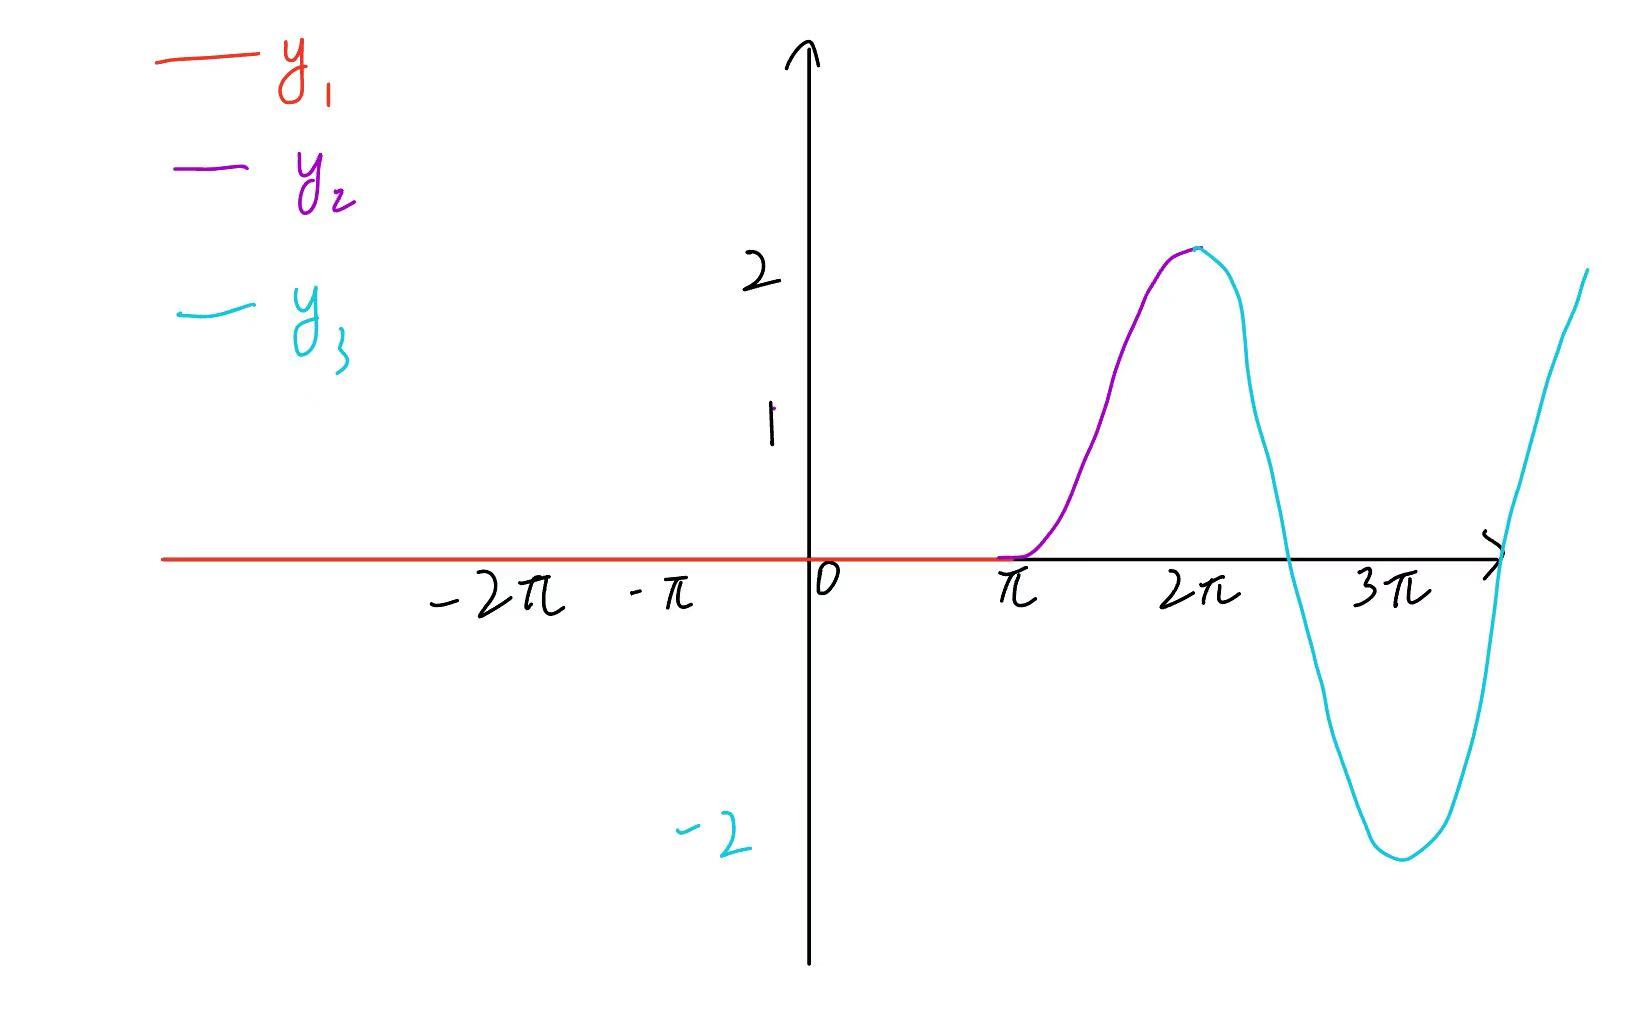
\includegraphics[width=10cm]{DE-ch3-10.jpg}
\end{figure}

\hrulefill

\subsubsection*{Solve
\begin{equation*}
    y''-4y=\delta(x-a)
\end{equation*}
where $\delta$ is the Dirac delta function, subject to the boundary conditions that $y$ is bounded as $|x|\to\infty$. Sketch the solution.}
\bf Solution. \normalfont $\delta(x-a)$ is defined as 
\begin{equation*}
    \begin{cases}
        0,\ x \neq a \\
        \text{"infinity", }x=a
    \end{cases}
\end{equation*}
and so, for $x\neq a$, we can treat the differential equation as
\begin{equation*}
    y''-4y=0
\end{equation*}
which yields solutions
\begin{equation*}
    y=Ae^{2x}+Be^{-2x}
\end{equation*}
for some constants $A$, $B$. The differential equation is split by the "asymptote" $x=a$; we will need to consider the cases $x<a$ and $x>a$ separately, noting that the two solutions in each case are continuous at $x=a$ (which makes physical sense, given that $\delta$ is used to model impulsive forces in physical systems). \\ \\
For $x<a$, the solution is bounded as $x\to -\infty$ and thus $B=0$ (as if $B$ was positive, the solution would exhibit exponential growth). Therefore we have 
\begin{equation*}
    y_1=Ae^{2x}\ (x<a)
\end{equation*}
For $x>a$, similar reasoning gives us $A=0$ and $y_2 = Be^{-2x}$. At $x=a$, with the understanding that the properties of the delta function can only be used inside integrals, we integrate both sides from $a^-$ to $a^+$:
\begin{equation*}
    \int^{a^+}_{a^-} y''-4y\ dx = \int^{a^+}_{a^-}\delta(x-a) = 1
\end{equation*}
by definition, with the left-hand side being 
\begin{equation*}
    [y']^{a^+}_{a^-} - 4\int^{a^+}_{a^-}y\ dx
\end{equation*}
where the second term is zero if $y$ is continuous (which we want it to be). $y'$ on the left-hand side of $a$ is $y_1' = 2Ae^{2x}$, and $y'$ on the right-hand side is $y_2'=-2Be^{2x}$; thus, we have 
\begin{equation*}
    -2Be^{-2a} - 2Ae^{2a} = 1
\end{equation*}
If $y_1$ and $y_2$ are part of the same continuous function, then $y_1(a^-)=y_2(a^+)$ and we also have 
\begin{equation*}
    Ae^{2a} = Be^{-2a}
\end{equation*}
and thus we obtain, when substituting into the previous equation, 
\begin{equation*}
    -4Ae^{2a}=1,\ A = -\frac{1}{4}e^{-2a}
\end{equation*}
and 
\begin{equation*}
    B = -\frac{1}{4}e^{2a}
\end{equation*}
yielding the solution
\begin{equation*}
    \begin{cases}
        -\frac{1}{4}e^{2(x-a)},\ x < a \\
        -\frac{1}{4}e^{2(a-x)},\ x >a
    \end{cases}
\end{equation*}
A sketch of the solution appears as follows:
\begin{figure}[h]
    \centering
    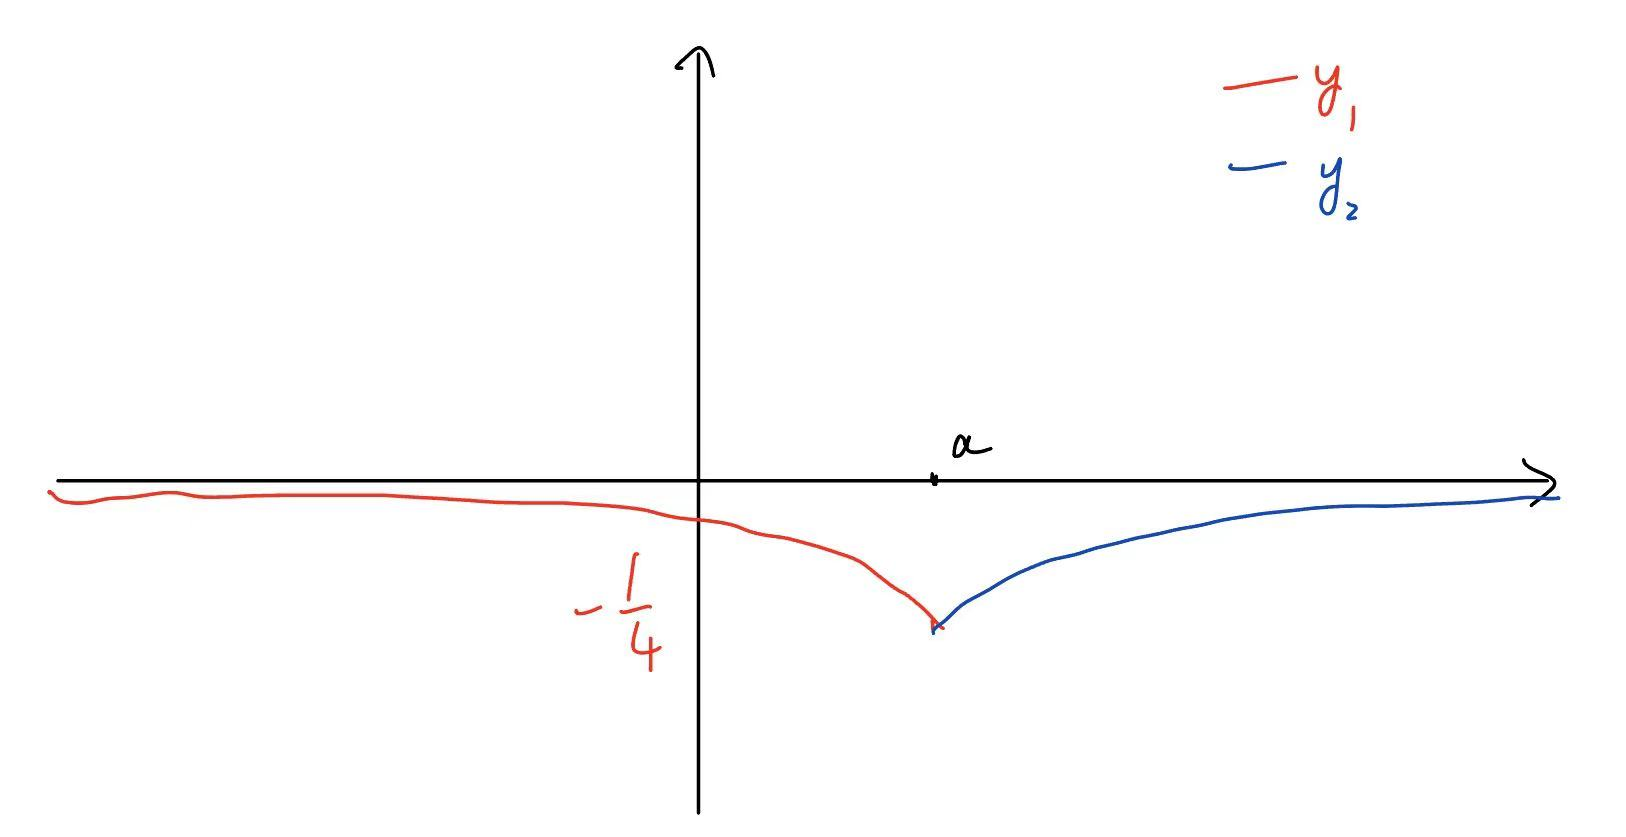
\includegraphics[width=10cm]{DE-ch3-11.jpg}
\end{figure}

\hrulefill

\subsubsection*{Solve
\begin{equation*}
    \ddot{y}+2\dot{y}+5y=2\delta(t)
\end{equation*}given that $y=0$ for $t<0$. Give an example of a physical system that this describes.}
\bf Solution. \normalfont The homogeneous equation yields
\begin{equation*}
    y =e^{-t}(A\sin t + B\cos t)
\end{equation*}
with the intervals $t < 0$ and $t > 0$ needing to be considered separately due to the presence of the delta function, which spikes at $t=0$. As the problem states, $y = 0$ for $t < 0$. At the point $t = 0$, we integrate from $t=0^-$ to $t=0^+$:
\begin{equation*}
    [\dot{y}]^{0^+}_{0^-} + 2[y]^{0+}_{0^-} +5\int^{0^+}_{0^-} y\ dt = 2\int^{0^+}_{0^-}\delta(t)\ dt = 2
\end{equation*}
with the final term on the left-hand side being 0 due to continuity; thus, with $\dot{y}$ on the right-hand side being
\begin{equation*}
    \dot{y} = -e^{-t}(A\sin t + B \cos t) + e^{-t}(A\cos t - B\sin t)
\end{equation*}
which evaluates to $A-B$ at $t=0$. $y(0^+)$ evaluates to $B$. Thus, we have
\begin{equation*}
    A-B+2B=A+B=2
\end{equation*}
from the above equation. We have assumed that $y$ is continuous, so in reality we want $y(0^+) = 0$ as $y(0^-) = 0$; thus, we conclude that $B=0$ and
\begin{equation*}
    y=2e^{-t}\sin t,\ t>0
\end{equation*}
This describes a spring with a load of mass 1 kg and spring constant 5, experiencing a damping force with damping coefficient 2 alongside an impulsive force of magnitude 2N at time $t=0$.

\hrulefill

\subsubsection*{Show that, for suitably chosen $P(x)$, the transformation $y(x)=P(x)v(x)$ reduces the equation \begin{equation*}
    y''+p(x)y'+q(x)y=0
\end{equation*}to the form
\begin{equation*}
    v''+J(x)v=0.\ (\dagger)
\end{equation*}
The sequence of functions $v_n$ is defined, for a given function $J(t)$ and in a given range $0\leq x \leq R$, by $v_0(x)=a+bx$ and 
\begin{equation*}
    v_n(x)=\int_{0}^{x} (t-x)J(t)v_{n-1}(t)\ dt.\ (n\geq 1).
\end{equation*}
Show that $v''_n(x)+J(x)v_{n-1}=0$ ($n\geq 1$) and deduce that $v(x) = \sum_{n=0}^{\infty}v_n(x)$ satisfies $(\dagger)$ with the initial conditions $v(0)=a$, $v'(0)=b$. What does this tell us about the existence problem for general second-order linear equations with given initial conditions?}
\bf Solution. \normalfont The first part of the problem is a reduction of order problem, one that's appeared several times; differentiating $y(x)=P(x)v(x)$ twice, plugging into the equation and setting $J(x)=-\frac{p(x)^2}{4}-\frac{p'(x)}{2}+q(x)$ will suffice to prove $(\dagger)$. \\ \\
To show that $v_n''(x)+J(x)v_{n-1}=0$, we examine the integral definition of $v_n(x)$:
\begin{equation*}
    v_n(x)=\int_{0}^{x} (t-x)J(t)v_{n-1}(t)\ dt=\int_{0}^{x} tJ(t)v_{n-1}(t)\ dt - x\int_{0}^{x} J(t)v_{n-1}(t)\ dt
\end{equation*}
and thus, by the Fundamental Theorem of Calculus, we have
\begin{equation*}
    v_n'(x) = xJ(x)v_{n-1}(x) - x(J(x)v_{n-1}(x)) - \int_{0}^{x}J(t)v_{n-1}(t)\ dt
\end{equation*}
where the first two terms cancel, and thus we have 
\begin{equation*}
    v_n''(x)=-J(x)v_{n-1}(x)
\end{equation*}
yielding $v_n''(x)+J(x)v_{n-1}=0$. Now return to $(\dagger)$: $v'' + J(x)v=0$. If $v$ is the infinite series $\sum_{n=0}^{\infty}v_n(x)$, then we have 
\begin{equation*}
    v''=\sum_{n=0}^{\infty}v_n''(x)=-J(x)\sum_{n=1}^{\infty}v_{n-1}(x)=-J(x)\sum_{n=0}^{\infty}v_n(x)=-J(x)v
\end{equation*}
as $v_0''(x)$ is $(a+bx)''=b'=0$ and does not need to be included in the infinite sum. Thus, $v$ satisfies $(\dagger)$; quickly plugging in $x=0$ and $v_0=ax+b$ yields $v(0)=a$ and $v'(0)=b$, as 
\begin{equation*}
    v_n(0)=\int_{0}^{0} (t-x)J(t)v_{n-1}(t)\ dt=0,\ n\geq 1
\end{equation*}
and
\begin{equation*}
    v_n'(0)=0J(0)v_{n-1}(0) - 0(J(0)v_{n-1}(0)) - \int_{0}^{0}J(t)v_{n-1}(t)\ dt=0,\ n\geq1
\end{equation*}
and thus 
\begin{equation*}
    v(0)=v_0(0)=a+b(0)=a,\ v'(0)=v_0'(0)=b
\end{equation*}
This tells us that, for any general second-order linear differential equation 
\begin{equation*}
    y''+p(x)y'+q(x)y=0
\end{equation*}
it is always possible to find some function $v(x)$ such that $y(x)=P(x)v(x)$ is a solution to the differential equation, and that $v(x)$ satisfies the arbitrary initial conditions 
\begin{equation*}
    \begin{cases}
        v(0)=a\\
        v'(0)=b
    \end{cases}
\end{equation*}
Alternatively, it could also be stated that any initial-value problem for $y'$ and $y$ involving a second-order linear differential equation has a solution.\\ \\
All of this comes with the caveat that the seris for $v(x)$ is convergent; this can be shown through induction, as follows. (The following proof is given by the problem itself). Suppose that $|J(x)|<m$ and $|v_0(x)|<A$ for the range of $x$ considered, where
\begin{equation*}
    v_n(x)=\int_{0}^{x} (t-x)J(t)v_{n-1}(t)\ dt
\end{equation*}
We claim that $|v_n(x)|\leq \frac{Am^n x^{2n}}{(2n)!}$ under these conditions, thus allowing for convergence to occur exponentially quickly. We begin with the base case $n=1$, where 
\begin{equation*}
    |v_1(x)|=|\int_{0}^{x} (t-x)J(t)v_0(t)\ dt| \leq |\int_{0}^{x} (t-x)Am\ dt| =\frac{Amx^2}{2!} 
\end{equation*}
satisfying the claim when $n=1$. Next, assume that for some $n=k$,
\begin{equation*}
    |v_k(x)|\leq \frac{Am^k x^{2k}}{(2k)!}
\end{equation*}
Then we would have
\begin{equation*}
    \begin{aligned}
        |v_{k+1}(x)|&=|\int_{0}^{x} (t-x)J(t)v_{k}(t)\ dt| \\
        &\leq |\int_{0}^{x}(t-x)m\frac{Am^k x^{2k}}{(2k)!}\ dt| \\
        &\leq \frac{Am^{k+1} x^{2k}}{(2k)!}|\int_{0}^{x}(t-x)\ dt| \\
        &\leq \frac{Am^{k+1} x^{2(k+1)}}{2(2k)!} \\
        &\leq \frac{Am^{k+1} x^{2(k+1)}}{(2k)!(2k+1)(2k+2)} \\
        &\leq \frac{Am^{k+1} x^{2(k+1)}}{(2(k+1))!}
    \end{aligned}
\end{equation*}
as desired. Thus, by mathematical induction, our original claim is true and the convergence of $v(x)$ is exponentially fast.

\hrulefill

\subsubsection*{\it The expanding universe. \bf Einstein's equations for a flat isotropic and homogeneous universe can be written as: 
\begin{equation*}
    \begin{cases}
        \frac{\ddot{a}}{a}=-\frac{4\pi}{3}(\rho+3p)+\frac{\Lambda}{3}\\
        H\equiv \frac{\dot{a}}{a} = (\frac{8\pi}{3}\rho + \frac{\Lambda}{3})^{\frac{1}{2}},
    \end{cases}
\end{equation*}
where $a$ is the scale factor measuring the expansion of the universe ($\dot{a}>0$), $\rho$ and $p$ are the time-dependent energy density and pressure of matter, $\Lambda$ is the cosmological constant and $H>0$ the Hubble parameter. \\ \\
Use these equations to establish the following: if $\Lambda \approx 0$ and $\rho+3p>0$, the acceleration $\ddot{a}<0$ and the graph of $a(t)$ must be concave downward, implying that at a finite time $a$ must reach $a=0$ (the big bang). Using the tangent of the graph at present time $t=t_0$, show that the age of the universe is bounded by $t_0<H^{-1}(t_0)$.}
\bf Solution. \normalfont If $\Lambda \approx 0$, we can ignore the $\Lambda$ term in both of the above equations:
\begin{equation*}
    \begin{cases}
        \frac{\ddot{a}}{a}=-\frac{4\pi}{3}(\rho+3p)\\
        H\equiv \frac{\dot{a}}{a} = (\frac{8\pi}{3}\rho)^{\frac{1}{2}},
    \end{cases}
\end{equation*}
and as we know additionally that $\rho+3p>0$,
\begin{equation*}
    \frac{\ddot{a}}{a}=-\frac{4\pi}{3}(\rho+3p)<0
\end{equation*}
Additionally, the Hubble parameter (being a square root) is always positive; we know that $\dot{a}>0$ for all $t$, so $a=\frac{\dot{a}}{H}$ is positive for all $t$. Hence, $\ddot{a}=-\frac{4\pi(\rho+3p)}{3} a$ and is negative. A graph of $a$ with positive $\dot{a}$ and negative $\ddot{a}$ is increasing at a decreasing rate; hence, it is concave down. If the graph of $a$ is concave downward, then as $t$ decreases, $a$ decreases at an increasing rate, implying that $a$ will continue to decrease until $a$ reaches 0. \\ \\
Assume that at time $t=0$, the Big Bang occurred ($a(0)=0$). At present time $t_0$, the tangent of the graph of $a$ against $t$ is $\dot{a}(t_0)$. We know by the Mean Value Theorem that in-between $t=0$ and $t=t_0$, there exists some $t=k$ such that the tangent at $t=k$, $\dot{a}(k)$, is equal to the gradient of the line connecting the points $(0, 0)$ and $(t_0, a(t_0))$ (the secant line). This gradient is equal to
\begin{equation*}
    \frac{a(t_0)}{t_0}
\end{equation*} However, $\dot{a}$ decreases as a function of $t$, implying that $\dot{a}(t_0)$ is smaller than any gradient of the graph for $t<t_0$, and that 
\begin{equation*}
    \dot{a}(t_0) < \dot{a}(k) = \frac{a(t_0)}{t_0}
\end{equation*}
Thus we have 
\begin{equation*}
    t_0 < \frac{a(t_0)}{\dot{a}(t_0)} = \frac{1}{H(t_0)}
\end{equation*}
as desired.\\ \\\
\subsubsection*{Consider the physical situations of a matter-dominated universe ($\Lambda, p \approx 0$) and a radiation-dominated universe ($\Lambda \approx 0, p=\frac{\rho}{3}$). In each case, reduce the two equations above to a single differential equation for $a$ which is homogenous in $t$, and then show that there is a solution of the type $a=t^{\alpha}$. Determine the value of $\alpha$ in each case and verify that $\ddot{a}<0$.}
\bf Solution. \normalfont In the matter-dominated universe ($\Lambda, p \approx 0$), we have:
\begin{equation*}
    \begin{cases}
        \frac{\ddot{a}}{a}=-\frac{4\pi}{3}(\rho)\\
        H\equiv \frac{\dot{a}}{a} = (\frac{8\pi}{3}\rho)^{\frac{1}{2}} = (-2\frac{\ddot{a}}{a})^{\frac{1}{2}},
    \end{cases}
\end{equation*}
and thus 
\begin{equation*}
    \frac{\dot{a}^2}{a\ddot{a}} = -2
\end{equation*}
which is homogenous in $t$, as if $a(t)$ is a solution, $a(\lambda t)$ for some constant $\lambda$ is also a solution:
\begin{equation*}
    \frac{(a(\lambda t)')^2}{a(\lambda t)a(\lambda t)''} = \frac{\lambda^2(a'(\lambda t))}{\lambda^2 a''(\lambda t) a(\lambda t)} = \frac{(a'(\lambda t))^2}{a''(\lambda t)a(\lambda t)}
\end{equation*}
which equals $-2$, as $a(t)$ satisfies the equation. When we plug in $a = t^{\alpha}$, we obtain:
\begin{equation*}
    \begin{aligned}
        \frac{\alpha^2 t^{2(\alpha - 1)}}{t^\alpha \alpha(\alpha - 1)t^{\alpha - 2}} &= -2 \\
        \frac{\alpha^2 t^{2(\alpha-1)}}{\alpha(\alpha - 1) t^{2(\alpha - 1)}} &= -2 \\
        \frac{\alpha}{\alpha - 1} &= - 2 \\
        3\alpha &= 2 \\
        \alpha &= \frac{2}{3}
    \end{aligned}
\end{equation*}
with $a(t)=t^{2/3}$. \\ \\
In the radiation-dominated universe, we have
\begin{equation*}
    \begin{cases}
        \frac{\ddot{a}}{a}=-\frac{8\pi}{3}(\rho)\\
        H\equiv \frac{\dot{a}}{a} = (\frac{8\pi}{3}\rho)^{\frac{1}{2}} = (-\frac{\ddot{a}}{a})^{\frac{1}{2}},
    \end{cases}
\end{equation*}
and thus 
\begin{equation*}
    \frac{(\dot{a})^2}{a\ddot{a}} = -1
\end{equation*}
with $a=t^{\alpha}$ yielding
\begin{equation*}
    \begin{aligned}
        \frac{\alpha}{\alpha - 1} &= -1 \\
        2\alpha &= 1 \\
        \alpha &= \frac{1}{2}
    \end{aligned}
\end{equation*}
similarly to before, with $a(t)=t^{1/2}$. In both these cases, $\ddot{a} < 0$ (negative coefficient of some power of a positive $a$). 

\subsubsection*{Now consider a $\Lambda$ dominated universe ($\rho, p << \Lambda$). Solve the differential equation for $a(t)$ and show that it corresponds to an accelerated universe ($\ddot{a}>0$) for $\Lambda >0$. This could describe the universe today and/or a very early period of exponential expansion known as inflation.}
In this case, we have 
\begin{equation*}
    \begin{cases}
        \frac{\ddot{a}}{a}\approx \frac{\Lambda}{3}\\
        H\equiv \frac{\dot{a}}{a} = (\frac{\Lambda}{3})^{1/2}=(\frac{\ddot{a}}{a})^{1/2} \\
        \frac{(\dot{a})^2}{\ddot{a}a}=1
    \end{cases}
\end{equation*}
where $a(t)\propto e^t$ would work, as all its derivatives are equal to itself; in this case, $\ddot{a}$ is clearly positive due to the exponential growth of $a$.
\newpage
\section{Series solutions to differential equations}
Up until this point, we've made many advances on the topic of linear differential equations. We now have a systematic method to determine the solutions of a constant-coefficient DE completely. Using various methods like the Wronskian, Abel's theorem, and variation of parameters, we can even determine particular solutions to any second-order linear DE. But what if the homogeneous equation we are considering does not have constant coefficients - for instance, equations like: 
\begin{equation*}
    4x^3y'' - (x^2+1)y' + xy = 0
\end{equation*}
For differential equations which do not have particularly "nice" (elementary) solutions, power series solutions are the best we can hope for - that is, solutions in the form
\begin{equation*}
    y=\sum_{n=0}^{\infty} c_n x^n
\end{equation*}
(or, equivalently, $c_n (x-x_0)^n$), for finite coefficients $c_0, c_1, \dots$, under the assumption that such a power series will converge. \\ \\
Before we begin our study of power series solutions to differential equations, we need to lay out a few basic principles regarding power series: namely, the notions of convergence/absolute convergence/divergence, the concept of the radius of convergence, and the application of the ratio test.
\begin{principle}
    (Convergence, absolute convergence, and divergence.) The power series
    \begin{equation*}
        y=\sum_{n=0}^{\infty} c_n (x-x_0)^n
    \end{equation*}
    is said to \it converge \normalfont at a point $x$ if the limit 
    \begin{equation*}
        \lim_{k\to\infty}\sum_{n=0}^{k} c_n (x-x_0)^n
    \end{equation*}
    exists; conversely, if the limit diverges to infinity, the power series is said to \it diverge.\normalfont \\ \\
    The power series is said to \it absolutely converge \normalfont at a point $x$ if the sum of the absolute value of all its terms 
    \begin{equation*}
        \lim_{k\to\infty}\sum_{n=0}^{k} |c_n (x-x_0)^n|
    \end{equation*}
    also converges. If a series is absolutely convergent at $x$, then it is also regularly convergent at $x$, though the converse is not necessarily true.
    There is a non-negative number $\rho$ such that, for all $|x-x_0|<\rho$, the series converges absolutely, and for all $|x-x_0|>\rho$, it diverges. Call $\rho$ the \it radius of convergence. \normalfont
\end{principle}
To determine the convergence of a power series, we can apply
\begin{method}
    (Ratio test.) For a fixed value of $x$ and for $a_n\neq 0$, consider the limit of the ratio between two consecutive terms: 
    \begin{equation*}
        \lim_{n\to\infty} |\frac{c_{n+1}(x-x_0)^{n+1}}{c_{n}(x-x_0)^n}|=\lim_{n\to\infty} |x-x_0||\frac{c_{n+1}}{c_n}|=\lim_{n\to\infty}|x-x_0|L
    \end{equation*}
    If this ratio is less than 1, the terms of the power series are shrinking and the series converges absolutely; if it is greater than 1, the terms are increasing and thus the series diverges. If the ratio is 1, then no conclusive statement can be made.
\end{method}
For a convergent power series, taking its derivative is equivalent to adding up the derivatives of all of its terms; that is,
\begin{equation*}
    y'=\sum_{n=0}^{\infty} (c_n (x-x_0)^n)'\ \ \ \ \  (=\sum_{n=0}^{\infty} nc_n (x-x_0)^{n-1})
\end{equation*}
implying that $y$ is infinitely differentiable at $x_0$. If $y$ indeed has a power series representation at $x=x_0$, we refer to $y$ as \it analytic\normalfont . This gives us everything we need to establish two more important classifications: ordinary and singular points. Let us return to the general form of our second-order linear DE:
\begin{equation*}
    p(x)y''+q(x)y'+r(x)y=0
\end{equation*}
which can also be written as 
\begin{equation*}
    y''+\frac{q(x)}{p(x)}y'+\frac{r(x)}{p(x)}y=0
\end{equation*}
We define
\begin{definition}
    (Singular and ordinary points.) If at a certain point $x_0$ the Taylor series (power series) for $\frac{q(x)}{p(x)}$ and $\frac{r(x)}{p(x)}$ do not exist - most commonly because $p(x_0)$ is zero - that point will be a \it singular point\normalfont. Conversely, if the Taylor series of both functions at $x=x_0$ do exist (the functions are analytic), then $x=x_0$ is an ordinary point.
\\ \\
    (Regular and irregular singularities.) Let $x_0$ be a singular point of the aforementioned DE. Then if $\frac{q(x)}{p(x)}$ contains no more than the first power of $(x-x_0)$ in its denominator when simplified, and $\frac{r(x)}{p(x)}$ contains no more than the second power $(x-x_0)^2$ in its denominator, $x=x_0$ is a regular singularity. Otherwise, we deem it to be an irregular singularity.
\end{definition}
Why is this so? For some singular points (namely, where $\frac{q(x)}{p(x)}$ and $\frac{r(x)}{p(x)}$ are undefined because $p(x)=0$ at $x=x_0$), the answer is obvious: the coefficients themselves are undefined, meaning that the differential equation would not make sense. However, if - as the definition of a regular singularity goes - the maximum power of $(x-x_0)$ is 2 in $\frac{r(x)}{p(x)}$, and 1 in $\frac{q(x)}{p(x)}$, the power series solution for the DE 
\begin{equation*}
    y=\sum_{n=0}^{\infty} c_n (x-x_0)^n
\end{equation*}
    can cancel out these powers of $(x-x_0)$ as long as the first few terms are zero. This leads us to the solution
\begin{equation*}
        y=\sum_{n=0}^{\infty} c_n (x-x_0)^{(n+\sigma)},
\end{equation*}
also known as a Frobenius series, where $\sigma$ can be any complex number with $c_0 \neq 0$. This allows us to "skip" the first few terms of the Taylor series, and cancel out these pesky $x-x_0$ terms in the denominator that result in dividing by zero. If instead the singularity is irregular, then the same method no longer applies; power series solutions may not exist, or may behave strangely, at that particular point. \\ \\
Finally, at ordinary points where everything is well-defined, analytic, and has power series expansions, we simply have two linearly independent solutions of the form 
\begin{equation*}
    y=\sum_{n=0}^{\infty} c_n(x-x_0)^n
\end{equation*}
about the point $x=x_0$. 
\begin{theorem}
    (Fuch's theorem). The second-order differential equation 
    \begin{equation*}
        y''+p(x)y'+q(x)y=g(x)
    \end{equation*}
    has a power series solution expressible in the form
    \begin{equation*}
        y=\sum_{n=0}^{\infty} c_n (x-x_0)^{(n+\sigma)}
\end{equation*}
    near $x=x_0$ if $p(x)$, $q(x)$ and $g(x)$ are analytic at that point, or that point is a regular singular point. If instead $x=x_0$ is an ordinary point, there exists two linearly independent solutions of the form 
    \begin{equation*}
        y=\sum_{n=0}^{\infty} c_n(x-x_0)^n.
    \end{equation*}
\end{theorem}
Let us present an example of the method of power series near an ordinary point. 
\begin{example}
    Find solutions as power series in $x$ of the differential equation
    \begin{equation*}
        y''+xy=0.
    \end{equation*}
    \bf Solution. \normalfont First, we note that $x=0$ is an ordinary point - $x$ is clearly analytic here. As such, the usual power series solution 
    \begin{equation*}
        y=\sum_{n=0}^{\infty} c_n(x)^n
    \end{equation*}
    will work in this case. Substituting into the equation yields 
    \begin{equation*}
        y''=\sum_{n=1}^{\infty} nc_n(x)^{n-1}
    \end{equation*}
    (note that the range of the sum has gone from $n=0$ to $n=1$, as the derivative of the first term in $y$, a constant, is zero). And thus:
    \begin{equation*}
        \sum_{n=2}^{\infty} n(n-1)c_n(x)^{n-2}
    \end{equation*}
    Substituting into the equation yields
    \begin{equation*}
        \sum_{n=2}^{\infty} n(n-1)c_n(x)^{n-2}+ \sum_{n=0}^{\infty} c_n(x)^{n+1} = 0.
    \end{equation*}
    We want to shift the ranges of the two sums so that they have the same range and can be merged into a single sum. Inspection gives the first sum as 
    \begin{equation*}
        \sum_{n=0}^{\infty} (n+2)(n+1)c_{n+2}x^n
    \end{equation*}
    and thus the left-hand side of the DE as 
    \begin{equation*}
        2c_2 + \sum_{n=1}^{\infty}((n+2)(n+1)c_{n+2}+c_{n-1})x^n = 0
    \end{equation*}
    It is important to note here that if a power series is zero, then all of its terms must be zero. Thus we can write: 
    \begin{equation*}
        \begin{cases}
            2c_2=0 \iff c_2 = 0 \\
            (n+2)(n+1)c_{n+2}+c_{n-1} = 0 \iff c_{n+2}=-\frac{c_{n-1}}{(n+1)(n+2)},\ n\geq 1
        \end{cases}
    \end{equation*}
    where two independent solutions arise from the values of $c_1$ and $c_2$.
\end{example}
\newpage
Let's now consider an example of solutions near a regular singular point.
\begin{example}
    Consider the differential equation 
    \begin{equation*}
        4xy''+2(1-x)y'-y=0.
    \end{equation*}
    Find solutions as power series in $x$. \\ \\
    \bf Solution. \normalfont First, we convert the above equation to a form with coefficient of $y''$ equal to 1:
    \begin{equation*}
        y''+\frac{(1-x)}{2x}y'-\frac{1}{4x}y = 0
    \end{equation*}
    $x=0$ is a regular singular point (as the power of $x$ in the denominators of $\frac{1-x}{2x}$ does not exceed 1, and in $\frac{1}{4x}$, it does not exceed 2). We know from the theorem above that there exists a solution of the form 
    \begin{equation*}
        y=\sum_{n=0}^{\infty}c_n x^{n+\sigma}
    \end{equation*}
    with corresponding 
    \begin{equation*}
        y'=\sum_{n=0}^{\infty}c_n(n+\sigma) x^{n+\sigma-1}, \ y'' =\sum_{n=0}^{\infty}c_n(n+\sigma)(n+\sigma -1)x^{n+\sigma-2}
    \end{equation*}
    Substituting into the equation gives:
    \begin{equation*}
        \sum_{n=0}^{\infty}[4c_n(n+\sigma)(n+\sigma-1)+2c_n(n+\sigma)]x^{n+\sigma-1} - \sum_{n=0}^{\infty}[2c_n(n+\sigma)+1]x^{n+\sigma} = 0
    \end{equation*}
    and thus 
    \begin{equation*}
        \begin{cases}
            [4c_0(\sigma)(\sigma-1)+2c_0(\sigma)]x^{\sigma}-1=0 \\
            \sum_{n=0}^{\infty}[2c_{n+1}(n+\sigma)(2(n+\sigma+1)+1)-2c_n(n+\sigma)-c_n]x^{n+\sigma} = 0
        \end{cases}
    \end{equation*}
    The first term, involving only $\sigma$, is known as the \it indicial equation \normalfont (determines the value of the index):
    \begin{equation*}
        4c_0(\sigma)(\sigma-1)+2c_0(\sigma) = 0 \iff \sigma(\sigma-1)+\frac{\sigma}{2}=0,\ \sigma=0,\ \frac{1}{2}
    \end{equation*}
    From the second term we obtain the recurrence relation
    \begin{equation*}
        2c_{n+1}(n+\sigma)(2(n+\sigma+1)+1)-2c_n(n+\sigma)-c_n=0
    \end{equation*}
    or equivalently
    \begin{equation*}
        c_{n+1}=\frac{1+2(n+\sigma)}{2(n+\sigma)(2(n+\sigma+1)+1)}c_n
    \end{equation*}
    where $\sigma = 0,\ \frac{1}{2}$ can be plugged in to obtain two independent solutions.
\end{example}
\newpage
\subsubsection{Resonance of solutions}
In the previous section, we mentioned the notion of an \it indicial equation \normalfont that determined the index of the Frobenius series in the case of a regular singular point. As with differential equations with constant coefficients, it may be that this indicial equation yields repeated roots or roots $\sigma_1,\ \sigma_2$ that have special characteristics. Let's examine these cases one by one:
\begin{enumerate}
    \item $\sigma_2-\sigma_1$ is not an integer. In this case, the two Frobenius series
    \begin{equation*}
        \sum_{n=0}^{\infty}c_n(x-x_0)^{n+\sigma_{1,2}}
    \end{equation*}
    are independent solutions to the differential equation. 
    \item $\sigma_2-\sigma_1$ is an integer (including when the two are equal). In this case, one series is contained within the other, so the Frobenius method cannot find two independent series. One independent solution will be 
    \begin{equation*}
        y_1=\sum_{n=0}^{\infty}c_n(x-x_0)^{n+\sigma_2}
    \end{equation*}
    for $\sigma_2\geq \sigma_1$, as dictated by the Frobenius series, but the other independent solution will usually be in the form
    \begin{equation*}
        y_2=\ln(x-x_0)y_1+\sum_{n=0}^{\infty}b_n(x-x_0)^{n+\sigma_2}
    \end{equation*}
\end{enumerate}
\newpage
\section{Multivariate differential equations}
\subsection{Directional derivatives}
In this subsection - as with this entire section - we will be focusing our efforts on the multivariate function $z=f(x,y)$ and all its generalized relatives: how we can bring our tools of calculus from two dimensions to three-dimensional space, and how differential equations operate within that space.\\ \\
 Before we can be concerned with differential equations, we have to concern ourselves with rates of change.
 \begin{definition}
    (Gradient for multivariate functions). Define $\nabla f$, the \it gradient \normalfont of $f(x,y)=z$, as the vector
    \begin{equation*}
        \begin{bmatrix}
            \frac{\partial f}{\partial x} \\
            \frac{\partial f}{\partial y}
        \end{bmatrix}
    \end{equation*}
    And for the generalized multivariate case, a matrix of partiaal derivatives of $f$ with respect to all its variables.
 \end{definition}
 Note that this is simply a definition; we haven't attached any geometric significance to the gradient yet, but we will - eventually. To get there, consider the following question. We know that $\frac{\partial f}{\partial y}$ gives us the rate of change of $f$ with small changes in $x$, and the partial derivative in $y$ with small changes in $y$; however, what if we choose to move not along one of the axes, but (as is possible in three dimensions) along a certain vector? For instance, take the unit vector
 \begin{equation*}
    \vec{s} = \begin{bmatrix}
        a \\ b
    \end{bmatrix}
 \end{equation*}
 for some $a$, $b$ with $\sqrt{a^2+b^2}=1$. If we're going to be moving along $\vec{s}$, then we'll be moving $a$ units in the $x$-direction and $b$ units in the $y$-direction. The partial derivatives give us how much $f$ changes when we move along each direction, so we can write 
 \begin{equation*}
    \frac{\partial f}{\partial s} = a\frac{\partial f}{\partial x} + b\frac{\partial f}{\partial y}
 \end{equation*}
 as the rate of change of $f$ along $\vec{s}$. Note that we can also rewrite the above as 
 \begin{equation*}
    \frac{\partial f}{\partial \vec{s}} = \nabla f \cdot \vec{s} \ (\text{notated }\nabla_{\vec{s}} f)
 \end{equation*}
 which gives us an insight on what the gradient represents: essentially, it is a vector representing the "base" rate of change at a point that all other directional derivatives are based off of. We also note that, since the dot product is maximized when $\cos \theta = 1$ and the angle $\theta$ between the two vectors equalling zero, the directional derivative is at a maximum when $\vec{s}$, the direction travelled in, is in the same direction as the gradient. Thus, the gradient is the direction that maximizes the rate of change of the function. If instead $\vec{s}$ is parallel to the gradient, then the directional derivative is zero. 
\subsection{Stationary points of multivariate functions}
Consider a point $(x,y)=(a,b)$ on the contours of the function $f(x,y)=z$; in particular, consider its gradient 
\begin{equation*}
    \nabla f = \begin{bmatrix}
        \frac{\partial f}{\partial x} (a,b) \\
        \frac{\partial f}{\partial y} (a,b)
    \end{bmatrix}.
\end{equation*}
If either partial derivative is nonzero, that implies that we can increase (or decrease) the value of $f$ by taking a small step in that direction; that tells us $(a,b)$ is not a stationary (maximum or minimum) point, as we can reach a higher or lower value of $f$ immediately next to $(a,b)$. Thus, our condition for a critical point is 
\begin{equation*}
    \nabla f = \vec{0}
\end{equation*}
or, equivalently, that all partial derivatives of $f$ are zero at that point. Much as univariate calculus gave rise to points of inflection, however, a special case arises where $\nabla f = 0$ but the point is not a stationary point; call these types of points \it saddle points.\normalfont \\ \\
\begin{figure}[h]
    \centering
    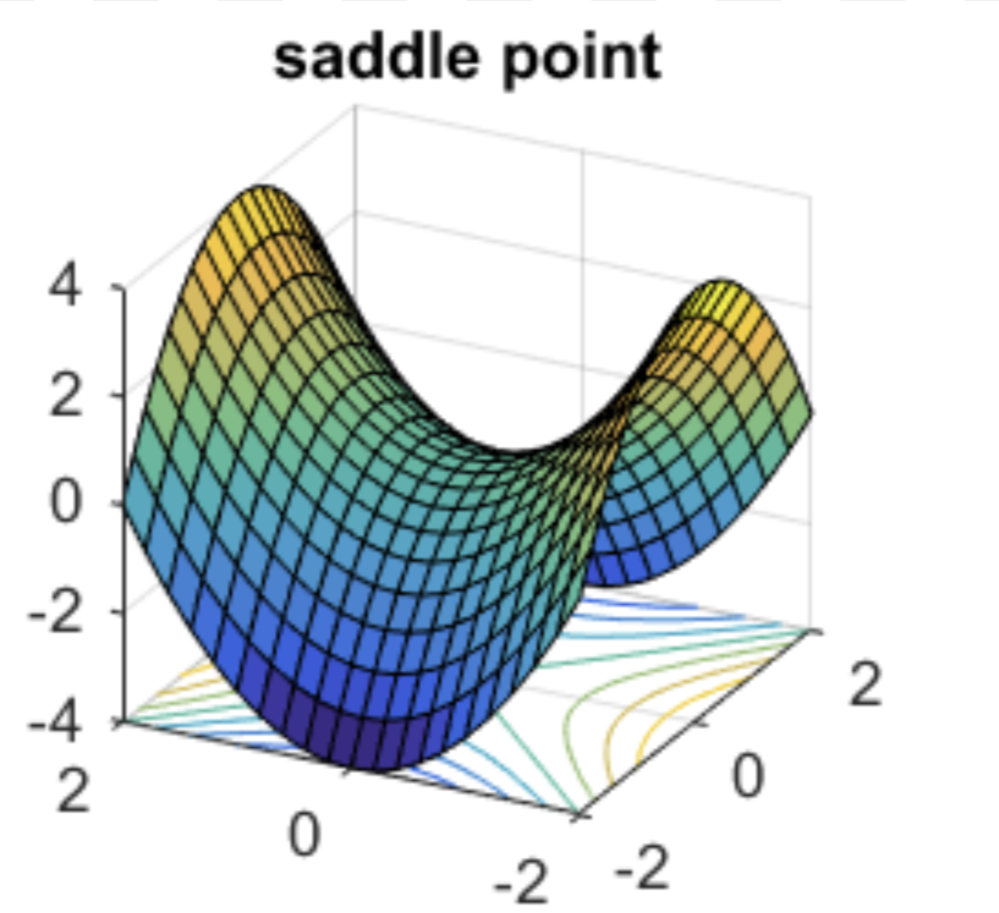
\includegraphics[width=8cm]{DE-ch4-saddlepoint.png}
\end{figure}
Why does this happen? The above graph might give us a bit of a clue; it is the graph of $f(x,y)=x^2-y^2$, with saddle point $(x,y)=(0,0)$. At that point, the function $f(x,0)=x^2$ and the function $f(0,y)=-y^2$ are minimized and maximized respectively; this means that at $(0,0)$, the function curves up in one direction and down in another direction, creating a point where the function is transitioning between turning up and down (similar to points of inflection).
\subsection{Taylor series for multivariate functions}
Consider a point $\vec{s_0}=(x_0,y_0)$ on $f(x,y)=f(\vec{s})=z$, and a small displacement $\delta \vec{s}=(\delta x, \delta y)$ from that point. We want to find an approximation, similar to the one we obtained for single-variable functions through Taylor series, for the value of:
\begin{equation*}
    f(x_0+\delta x, y_0+\delta y) = f(\vec{s_0}+\delta \vec{s})
\end{equation*}
Let $x = x_0 + \delta x$, $y=y_0 + \delta y$. We'll consider the terms of the approximation one by one. The first term, as is know by Taylor's theorem, is simply $f(x_0,y_0)$. The second term should be equal to the change in $(x_0,y_0)$ multiplied by its rate of change - in multidimensional terms, this is the directional derivative of $\begin{bmatrix}
    x-x_0\\y-y_0
\end{bmatrix}=\delta \vec{s}$:
\begin{equation*}
    f(x,y)=f(x_0,y_0)+\nabla_{\delta \vec{s} f} =f(x_0,y_0)+[(x-x_0)\frac{\partial f}{\partial x} + (y-y_0)\frac{\partial f}{\partial y}].
\end{equation*}
By Taylor's theorem, the quadratic term will be $\frac{1}{2!}$ times the change in $x$ and $y$, $\delta \vec{s}$, times the second directional derivative in that direction. This is given by 
\begin{equation*}
    \begin{aligned}
        \frac{1}{2!}(\nabla_{\delta \vec{s}}\nabla_{\delta \vec{s}})f &= \frac{1}{2!}\nabla_{\delta \vec{s}}[(x-x_0)\frac{\partial f}{\partial x} + (y-y_0)\frac{\partial f}{\partial y}] \\
        &= \frac{1}{2!}\delta \vec{s}\cdot \nabla([(x-x_0)\frac{\partial f}{\partial x} + (y-y_0)\frac{\partial f}{\partial y}])\\
        &= \frac{1}{2!}\delta \vec{s}\cdot\begin{bmatrix}
            (x-x_0)\frac{\partial^2 f}{\partial x^2} +(y-y_0)\frac{\partial^2 f}{\partial x \partial y}\\
            (y-y_0)\frac{\partial^2 f}{\partial y^2}+(x-x_0)\frac{\partial^2 f}{\partial x \partial y}
        \end{bmatrix} \\
        &= \frac{1}{2!}[(x-x_0)^2 \frac{\partial^2 f}{\partial x^2} + 2(x-x_0)(y-y_0)\frac{\partial^2 f}{\partial x \partial y}+(y-y_0)\frac{\partial^2 f}{\partial y^2}]
    \end{aligned}
\end{equation*}
Note that $(x-x_0)$ and $(y-y_0)$ are not treated as variables in the above because they are $\delta x$ and $\delta y$, independent from $x$ and $y$. According to the above, we define 
\begin{definition}
    (Hessian matrix). The \it Hessian matrix \normalfont for $f(x,y)$ is the matrix
    \begin{equation*}
        \nabla \nabla f = \begin{bmatrix}
            f_{xx} & f_{xy} \\
            f_{yx} & f_{yy}
        \end{bmatrix}
    \end{equation*}
    such that the above quadratic term in the Taylor expansion for $f(x,y)$ can also be written 
    \begin{equation*}
        \frac{1}{2!}\begin{bmatrix}
            \delta x & \delta y
        \end{bmatrix}\nabla \nabla f \begin{bmatrix}
            \delta x \\ \delta y
        \end{bmatrix}.
    \end{equation*}
\end{definition}
The Hessian matrix encodes information about the second-order partial derivatives for $f$. It can be generalized for $f(x_1,x_2,\dots,x_n)$, a multivariate function in $n$ variables, as 
    \begin{equation*}
        \nabla \nabla f = \begin{bmatrix}
            f_{x_1x_1} & f_{x_1x_2} & \dots & f_{x_1x_n} \\
            f_{x_2x_1} & f_{x_2x_2} & \dots & f_{x_2x_n} \\
            \vdots & \vdots & \vdots & \vdots \\
            f_{x_nx_1} & f_{x_n x_2} & \dots & f_{x_nx_n}
        \end{bmatrix}
    \end{equation*}
    and the Taylor expansion term as 
    \begin{equation*}
        \frac{1}{2!}(\delta s)^{\mathbf{T}}\nabla \nabla f (\delta s).
    \end{equation*}
    where 
    \begin{equation*}
        \delta s = \begin{bmatrix}
            \delta x_1 \\ \delta x_2 \\ \vdots \\ \delta x_n
        \end{bmatrix}
    \end{equation*}
    and the $\mathbf{T}$ indicates matrix transposition.
\subsection{Classification of multivariate stationary points}
\begin{theorem}
    (Hessian determinant test.) The Hessian determinant test for classifying stationary points of multivariate functions is as follows. Let $H = \nabla \nabla f(x,y)$ be the Hessian matrix as defined above:
    \begin{equation*}
        H = \begin{bmatrix}
            f_{xx} & f_{xy} \\
            f_{yx} & f_{yy}
        \end{bmatrix}
    \end{equation*}
    If the point $(x_0,y_0)$ with associated Hessian $H(x_0,y_0)$ is a stationary point, then we can classify its nature as follows:
    \begin{equation*}
        \begin{cases}
            \det H>0,\ f_{xx}(x_0,y_0) > 0: \text{ $(x_0, y_0)$ is a minimum.}\\
            \det H>0,\ f_{xx}(x_0,y_0) < 0: \text{ $(x_0, y_0)$ is a maximum.}\\
            \det H<0: \text{ $(x_0, y_0)$ is a saddle point.}\\
            \det H = 0: \text{ the point is indeterminate in nature.}
        \end{cases}
    \end{equation*}
    We can also refer to this test through the \it signature \normalfont of the Hessian, which will be useful in higher-dimensional cases. For an $n$-variable Hessian matrix in $(x_1,x_2,\dots,x_n)$, let its signatures be
    \begin{equation*}
        f_{x_1 x_1},\ \begin{vmatrix}
            f_{x_1x_1} & f_{x_1x_2}\\
            f_{x_2x_1} & f_{x_2x_2}
        \end{vmatrix},\ \dots,\ \begin{vmatrix}
            f_{x_1x_1} & f_{x_1x_2} & \dots & f_{x_1x_n} \\
            f_{x_2x_1} & f_{x_2x_2} & \dots & f_{x_2x_n} \\
            \vdots & \vdots & \vdots & \vdots \\
            f_{x_nx_1} & f_{x_n x_2} & \dots & f_{x_nx_n}
        \end{vmatrix}
    \end{equation*}
    Name these terms $H_1, H_2, \dots, H_n$ respectively. If $H_1, H_2, \dots, H_n$ have signs $+, +, \dots, +$ (all positive) at a certain stationary point, then the point is a local minimum; if the signatures are $-, +, -, \dots, +, \dots$ (alternating signs starting with negative), then the point is a local maximum. Otherwise, if the determinant is not zero, the point is a saddle point.
\end{theorem}
Why does this hold true? It is beyond our abilities to provide a full proof at the moment, but using the tools of eigenvalues in linear algebra, we can provide an intuitive explanation for all of this. We first note that $H$ is "symmetric" no matter how many dimensions or variables there are; when we flip it around the diagonal, it remains the same because for a continuous function, $f_{xy}=f_{yx}$. (This symmetry is most evident in the two-dimensional case). A result from linear algebra tells us that because of this symmetry, $H$ can be diagonalized, i.e. it can be written in terms of its eigenvalues:
\begin{equation*}
    (\delta \vec{s})^{\mathbf{T}}\cdot H\cdot \delta\vec{s} = \begin{bmatrix}
        \delta x_1 & \delta x_2 & \dots & \delta x_n 
    \end{bmatrix}\begin{bmatrix}
        \lambda_1 & & & \\
        & \lambda_2 & & \\
        & & \ddots & \\
        & & & \lambda_n
    \end{bmatrix}\begin{bmatrix}
        \delta x_1 \\ \delta x_2 \\ \dots \\ \delta x_n 
    \end{bmatrix}
\end{equation*}
which then equals the sum
\begin{equation*}
    \lambda_1(\delta x_1)^2+\lambda_2(\delta x_2)^2 + \dots + \lambda_n(\delta x_n)^2
\end{equation*}
where $\lambda_1, \lambda_2, \dots$ denote the eigenvalues of $H$. This is relevant because the above term, $(\delta \vec{s})^{\mathbf{T}}\cdot H\cdot \delta\vec{s}$, is a part of the Taylor expansion of $f$:
\begin{equation*}
    f(x_1+\delta x_1, x_2+\delta x_1, \dots, x_n+\delta x_n) =f(x_1, x_2, \dots, x_n) + \delta\vec{s} \cdot \nabla f +  \frac{1}{2} (\delta \vec{s})^{\mathbf{T}}\cdot H\cdot \delta\vec{s}
\end{equation*}
with $\nabla f$ being 0 at any stationary point, so 
\begin{equation*}
    f(x_1+\delta x_1, x_2+\delta x_1, \dots, x_n+\delta x_n) =f(x_1, x_2, \dots, x_n) + \frac{1}{2} (\delta \vec{s})^{\mathbf{T}}\cdot H\cdot \delta\vec{s}
\end{equation*}
If the point $(x_1, x_2, ..., x_n)$ is a minimum, then we can expect any point close to it to be greater than it; thus, the last term in the above equation must be positive. Conversely, if the point is instead a minimum, any point next to it must be smaller than it, and the last term is a negative. We know that the last term is the sum
\begin{equation*}
    \lambda_1(\delta x_1)^2+\lambda_2(\delta x_2)^2 + \dots + \lambda_n(\delta x_n)^2
\end{equation*}
which is positive if every eigenvalue is positive (minimum point), negative if every eigenvalue is negative (maximum point), and indeterminate if the signs are mixed (saddle point). This information about eigenvalues, as will become evident in the Linear Algebra course, is encoded within the determinant of the Hessian.
\newpage
\section{Systems of differential equations}
\subsection{Linear systems of differential equations}
\subsubsection{Transforming higher-order differential equations into systems}
Consider the generalized higher-order (constant-coefficient) differential equation:
\begin{equation*}
    y^{(n)}(x)+a_{n-1}y^{(n-1)} + \dots + a_2 y''(x) + a_1y'(x)+a_0 y = g(x)
\end{equation*}
Is there any way for us to simplify this into something easier to calculate? It turns out we need only to use a system of equations, with a set of $n$ new variables:
\begin{equation*}
    \begin{cases}
        y_1 = y \\
        y_2 = y_1'\ (=y') \\
        y_3 = y_2'\ (=y'')\\
        \dots \\
        y_n = y_{n-1}' (=y^{(n-1)}) \\        
    \end{cases}
\end{equation*}
and thus we have, from the generalized equation above, 
\begin{equation*}
    \begin{aligned}
        y_n' &= -a_{n-1}y^{(n-1)} - \dots - a_2 y''(x) - a_1y'(x)-a_0y \\
        &=-a_{n-1}y_n - \dots - a_2y_3 - a_1y_2 - a_0y_1
    \end{aligned}
\end{equation*}
with each equation being a first-order differential equation (no derivatives above the first derivative of each $y_k$). In essence, we have transformed an $n$th-order DE into a system of $n$ first-order DEs. Calling this a simplification of the original equation might seem the same as saying that topologically speaking, a coffee mug is equivalent to a donut, but observe the spark of genius lurking beneath the mundane waters of these blessed equations. As it turns out, it is extremely easy to rewrite these equations in matrix form: 
\begin{equation*}
    \frac{d}{dx}\begin{bmatrix}
        y_1\\
        y_2\\
        y_3\\
        \vdots\\
        y_n
    \end{bmatrix}=
    \begin{bmatrix}
        0 & 1 & 0 & \dots & 0 \\
        0 & 0 & 1 & \dots & 0 \\
        \vdots & \vdots & \ddots & \vdots & \vdots \\
        0 & 0 & 0 & \dots & 1 \\
        -a_0 & -a_1 & -a_2 & \dots & -a_{n-1}
    \end{bmatrix}
    \begin{bmatrix}
        y_1\\
        y_2\\
        y_3\\
        \vdots\\
        y_n
    \end{bmatrix} + 
    \begin{bmatrix}
        0\\
        0\\
        0\\
        \vdots\\
        g(x)
    \end{bmatrix}
\end{equation*}
(We did this all the way back in Example Sheet 3, Problem 2!) \\ \\
Or, alternatively, writing the matrix on the left-hand side as $\mathbf{x}$, the first matrix on the right-hand side as $\mathbf{A}$, and the second matrix as $\mathbf{F}$, we have (simply!):
\begin{equation*}
    \dot{\mathbf{x}} = \mathbf{A}\mathbf{x} + \mathbf{F}
\end{equation*}
This is what would happen if linear algebra and differential equations went to a party together (only hypothetically speaking, since mathematicians aren't invited to parties), got aggressively drunk, found themselves tangled within each other's luscious locks, and birthed a love-child through mitosis; it's where the two converge, and it's where we can study both together. The rest of this section will be entirely focused on the study of systems of this form.
\subsubsection{Eigenvalue solutions to systems of differential equations}
How do we begin to solve systems of the form 
\begin{equation*}
    \dot{\mathbf{x}} = \mathbf{A}\mathbf{x} + \mathbf{F}?
\end{equation*}
To gain a foothold on these, let's consider the most simple case of all: a case where we simply have 
\begin{equation*}
    \mathbf{F} = 0
\end{equation*}
yielding a homogeneous equation, and 
\begin{equation*}
    \mathbf{A}=\begin{bmatrix}
        a_1 & 0 & \dots & 0 & 0 \\
        0 & a_2 & \dots & 0 & 0 \\
        \vdots & \vdots & \ddots & \vdots & \vdots \\
        0 & 0 & \dots & a_{n-1} & 0 \\
        0 & 0 & \dots & 0 & a_n
    \end{bmatrix}
\end{equation*}
resulting in the system of equations 
\begin{equation*}
    \begin{cases}
        y_1' = a_1 y_1 \\
        y_2' = a_2 y_2 \\
        \dots \\
        y_n' = a_n y_n
    \end{cases}
\end{equation*}
all of which are solvable as $y_k = Ae^{a_k x}$. If we can focus our efforts in transforming the general case $\dot{\mathbf{x}} = \mathbf{A}\mathbf{x} + \mathbf{F}$ into this simplified (and directly solvable) case, we'll have figured out a method to solve many systems of differential equations. Note that in the simplified case, the matrix $\mathbf{A}$ is diagonal; our end goal should therefore be to convert every matrix $\mathbf{A}$ into a diagonal matrix, too - one that gives us precisely the scale factor of the matrix along every axis, and nothing else. \\ \\
As it turns out, we know precisely how to do that. Suppose that $\mathbf{A}$ has $n$ eigenvalues $\lambda_{1,2,\dots,n}$ satisfying $\det |A-\lambda I|=0$. Define the eigenvalue matrix $\Lambda$ as the diagonal matrix
\begin{equation*}
    \Lambda=\begin{bmatrix}
        \lambda_1 & & & \\
        &\lambda_2 & & \\
        & & \ddots & \\
        & & & \lambda_n
    \end{bmatrix}
\end{equation*}
and define $\mathbf{V}$ as the matrix of eigenvectors $v_1, v_2, \dots, v_n$, each $n \times 1$, correspodning to $\lambda_{1,2,\dots,n}$:
\begin{equation*}
    \mathbf{V} = \begin{bmatrix}
        v_1 & v_2 & \dots & v_n
    \end{bmatrix}
\end{equation*}
We know that, by definition, $Av_k = \lambda_k v_k$. Thus, we have 
\begin{equation*}
    \begin{aligned}
        \mathbf{V \Lambda} &= \begin{bmatrix}
            \lambda_1 v_1 & \lambda_2 v_2 & \dots & \lambda_n v_n
        \end{bmatrix}\\
        &=\begin{bmatrix}
            v_1(1)\lambda_1 & v_2(1)\lambda_2 & \dots & v_n(1)\lambda_n \\
            v_1(2)\lambda_1 & v_2(2) \lambda_2 & \dots & v_n(2) \lambda_n \\
            \vdots & \vdots & \ddots & \vdots \\
            v_1(n) \lambda_1 & v_2(n) \lambda_2 & \dots & v_n(n)\lambda_n
        \end{bmatrix} \\
        &= \begin{bmatrix}
            \lambda_1v_1 & \lambda_2v_2 & \dots & \lambda_n v_n
        \end{bmatrix}\\
        &=\begin{bmatrix}
            Av_1 & Av_2 & \dots & Av_n
        \end{bmatrix}\\
        &=\mathbf{AV}
    \end{aligned}
\end{equation*}
where $v_i(j)$ denotes the $j$th-row element of vector $v_i$. As such, we have $\mathbf{AV=V\Lambda}$ and finally 
\begin{equation*}
    \mathbf{A= V\Lambda V^{-1}},\ \mathbf{\Lambda = V^{-1}AV}
\end{equation*}
for invertible $\mathbf{V}$; this is the process of \it diagonalization, \normalfont and it allows us to convert any matrix into a diagonal matrix of eigenvectors $\mathbf{\Lambda}$ by multiplying it with two other matrices.\\ \\
How does this help our cause in solving systems of differential equations? We return to 
\begin{equation*}
    \dot{\mathbf{x}} = \mathbf{A}\mathbf{x} + \mathbf{F}
\end{equation*}
and consider only the homogeneous case for a moment (like we do for normal differential equations):
\begin{equation*}
    \dot{\mathbf{x}} = \mathbf{A}\mathbf{x}
\end{equation*}
Let us impose the change of coordinates $x = \mathbf{Tz}$ for some $n \times n$ matrix $\mathbf{T}$, and $n\times 1$ matrix $\mathbf{z}$. Thus we have 
\begin{equation*}
    \mathbf{T\dot{z}} = \mathbf{A}\mathbf{Tz}
\end{equation*}
and 
\begin{equation*}
    \mathbf{\dot{z}} = \mathbf{T^{-1}}\mathbf{A}\mathbf{Tz}
\end{equation*}
which is just our equation for a diagonal matrix of eigenvectors above! Thus we take $\mathbf{T} = \mathbf{V}$, the matrix of eigenvectors for $\mathbf{A}$, and obtain simply 
\begin{equation*}
    \mathbf{\dot{z}} = \mathbf{\Lambda} \mathbf{z} = \begin{bmatrix}
        \lambda_1 & & & \\
        & \lambda_2 & & \\
        & & \ddots & \\
        & & & \lambda_n
    \end{bmatrix}\mathbf{z}
\end{equation*}
which gives solutions $z_1 = c_1e^{\lambda_1 x},\ z_2 = c_2e^{\lambda_2 x}, \dots, z_n = c_ne^{\lambda_n x}$ with $\mathbf{x=Vz}$, $\mathbf{V}$ as the eigenvector matrix of $\mathbf{A}$, and $\lambda_{1,2,\dots,n}$ as the eigenvalues of $\mathbf{A}$. In other words, we have
\begin{equation*}
    \begin{aligned}
        \mathbf{x} &= \mathbf{Vz}\\
        &= \begin{bmatrix}
            v_1 & v_2 & \dots & v_n
        \end{bmatrix}\begin{bmatrix}
            c_1e^{\lambda_1 x} \\
            c_2 e^{\lambda_2 x} \\
            \vdots \\
            c_ne^{\lambda_n x}
        \end{bmatrix}\\ \\
        &=\begin{bmatrix}
            v_1(1) & v_2(1) & \dots & v_n(1) \\
            v_1(2) & v_2(2) & \dots & v_n(2) \\
            \vdots & \vdots & \ddots & \vdots \\
            v_1(n) & v_2(n) & \dots & v_n(n)
        \end{bmatrix}
        \begin{bmatrix}
        c_1e^{\lambda_1 x} \\
        c_2 e^{\lambda_2 x} \\
        \vdots \\
        c_ne^{\lambda_n x}
        \end{bmatrix}\\ \\
        &=\begin{bmatrix}
            v_1(1)c_1e^{\lambda_1 x} + v_2(1)c_2 e^{\lambda_2 x} + \dots + v_n(1)c_ne^{\lambda_1 x} \\
            v_1(2)c_1e^{\lambda_1 x} + v_2(2)c_2 e^{\lambda_2 x} + \dots + v_n(2)c_ne^{\lambda_1 x} \\
            \dots \\
            v_1(n)c_1e^{\lambda_1 x} + v_2(n)c_2 e^{\lambda_2 x} + \dots + v_n(n)c_ne^{\lambda_1 x} \\
        \end{bmatrix}\\ \\
        &= c_1e^{\lambda_1 x }v_1 + c_2e^{\lambda_2 x}v_2 + \dots + c_ne^{\lambda_n x}v_n
    \end{aligned}
\end{equation*}
Which is the sum of all $e^{\lambda_k x}$ multiplied by their respective eigenvectors. This is the crucial link between eigenvalues and systems of differential equations; however, it is important to note that not all matrices are as nicely diagonalizable as the generalized example shown above. Matrices may have less than $n$ unique eigenvalues, or have complex eigenvalues, or so on. \\ \\
There also exists another avenue towards the conclusion that eigenvalues are linked to systems of differential equations. Suppose we know, by divine inspiration, that functions of the form $y_k=Ae^{\lambda_k x}$ for $k=1,2,\dots,n$ were needed to solve the system $\dot{\mathbf{x}} = \mathbf{A}\mathbf{x}$ (a reasonable assumption to make, since every equation in the system is a linear sum of $y_1, y_2, \dots, y_n$ and their derivatives, and so we want $y_k$ and $y_k'$ to be in the same form). Let us assume, then, that 
\begin{equation*}
    \mathbf{x} = \mathbf{v}e^{\lambda x}
\end{equation*}
for some vector $\mathbf{v}$, and thus $\mathbf{\dot{x}} = \lambda \mathbf{x}$. Substituting into $\mathbf{\dot{x}} = \mathbf{Ax}$, we have 
\begin{equation*}
    \lambda \mathbf{x} = \mathbf{Ax}
\end{equation*}
which is the defining equation for eigenvalues of the matrix $\mathbf{A}$, and corresponding eigenvectors $\mathbf{v}$. Thus, the solution to the system is the sum of all
\begin{equation*}
    \mathbf{x} = \mathbf{v}e^{\lambda x}
\end{equation*}
with $\lambda$ an eigenvalue of $\mathbf{A}$ and $v$ a corresponding eigenvector - the same solution as the one we found above through diagonalization.
\subsubsection{Phase-portrait analysis of linear systems}
Recall that our solution to the linear system of differential equations 
\begin{equation*}
    \mathbf{\dot{x}} = \mathbf{Ax}
\end{equation*}
was the sum of eigenvector products
\begin{equation*}
    \mathbf{x}=c_1e^{\lambda_1 x }v_1 + c_2e^{\lambda_2 x}v_2 + \dots + c_ne^{\lambda_n x}v_n
\end{equation*}
Let us write this in the form 
\begin{equation*}
    \mathbf{x} =y_1v_1 + y_2 v_2 + \dots y_n v_n.
\end{equation*}
Eigenvectors are extremely valuable to us because they are essentially the "axes" upon which our solution $\mathbf{x}$ acts on - if we vary only a single variable $y_k$, then we know that the solution has only changed along the eigenvector $v_k$. This allows us to build up a "phase-portrait" of our solution $\mathbf{x}$: a graph of how the vector $\mathbf{x}$ changes as $y_1, y_2, \dots, y_n$ vary, taking these as our axes. For our sanity's sake, let's consider only the two-dimensional case (with $y_1$ and $y_2$ as axes) and analyze the differing examples that arise out of the different forms of $y_1$ and $y_2$:
\subsubsection*{Sinks and sources}
Consider the case where $y_1 = c_1e^{\lambda_1 x}, y_2 =c_2e^{\lambda_2 x}$ have real eigenvalues $\lambda_1$, $\lambda_2$ with the same sign: $\lambda_1\lambda_2>0$. \\ \\
If both eigenvalues are negative, then both $y_1$ and $y_2$ are exponentially decaying functions; as the value of $x$ grows, $y_1$ and $y_2$ become smaller and smaller multiples of $v_1$ and $v_2$ and eventually move \it towards \normalfont the origin. Points like these are known as "stable sinks", or simply sinks:
\begin{figure}[h]
    \centering
    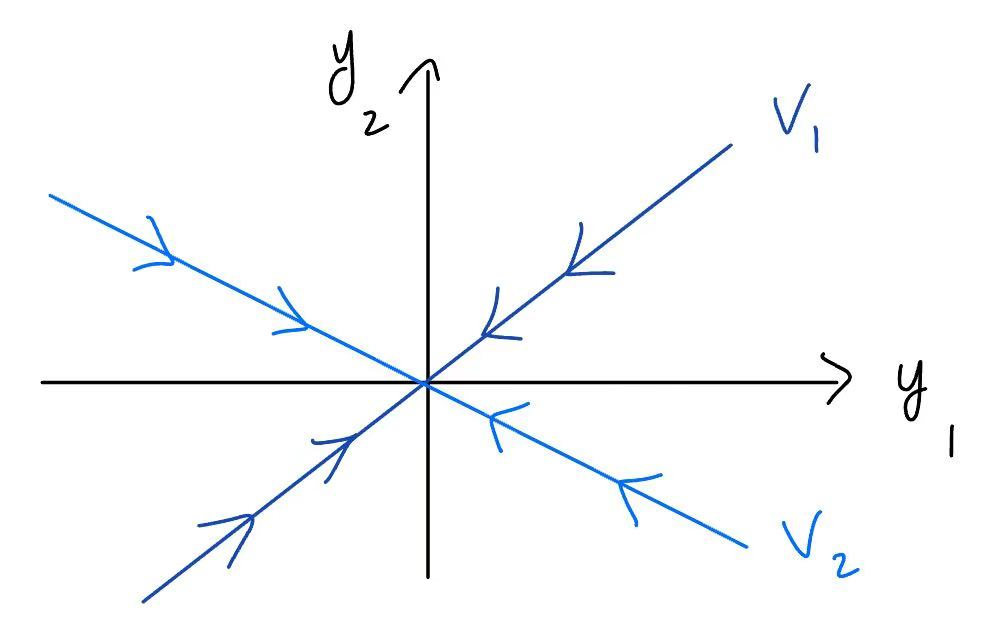
\includegraphics[width=8cm]{DE-ch4-stablesink.jpg}
\end{figure}
If both eigenvalues are instead positive, both $y_1$ and $y_2$ grow exponentially and thus travel \it away \normalfont from the origin when $x$ gets large, causing the arrows to point outward instead. We call this an \it unstable source \normalfont point:\newpage
\begin{figure}[h]
    \centering
    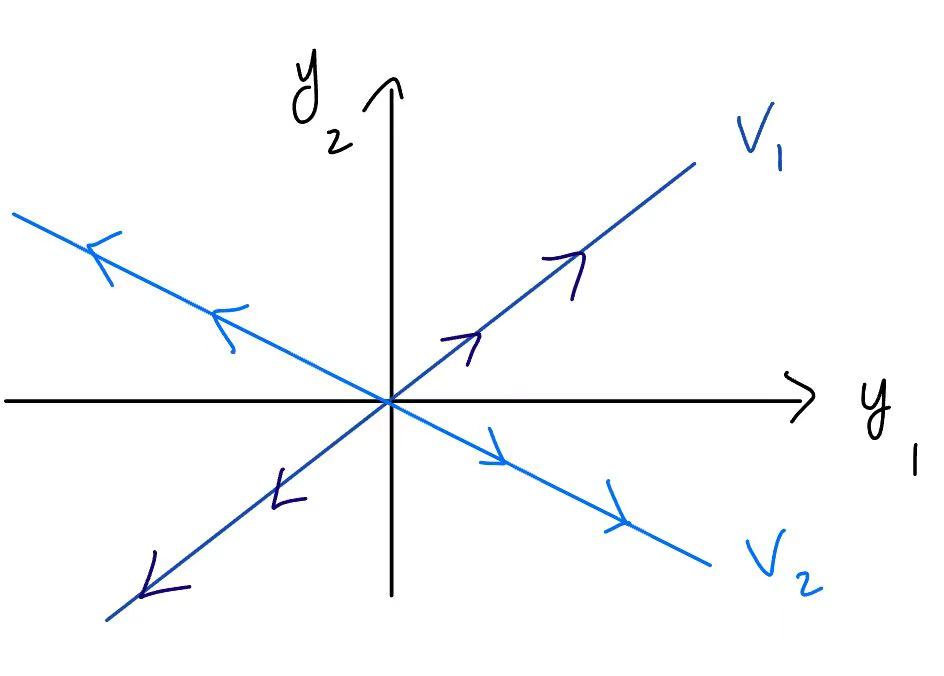
\includegraphics[width=8cm]{DE-ch4-unstablesource.jpg}
\end{figure}
Other vectors close to the eigenvectors can be drawn asymptotically to the eigenvectors, as shown:
\begin{figure}[h]
    \centering
    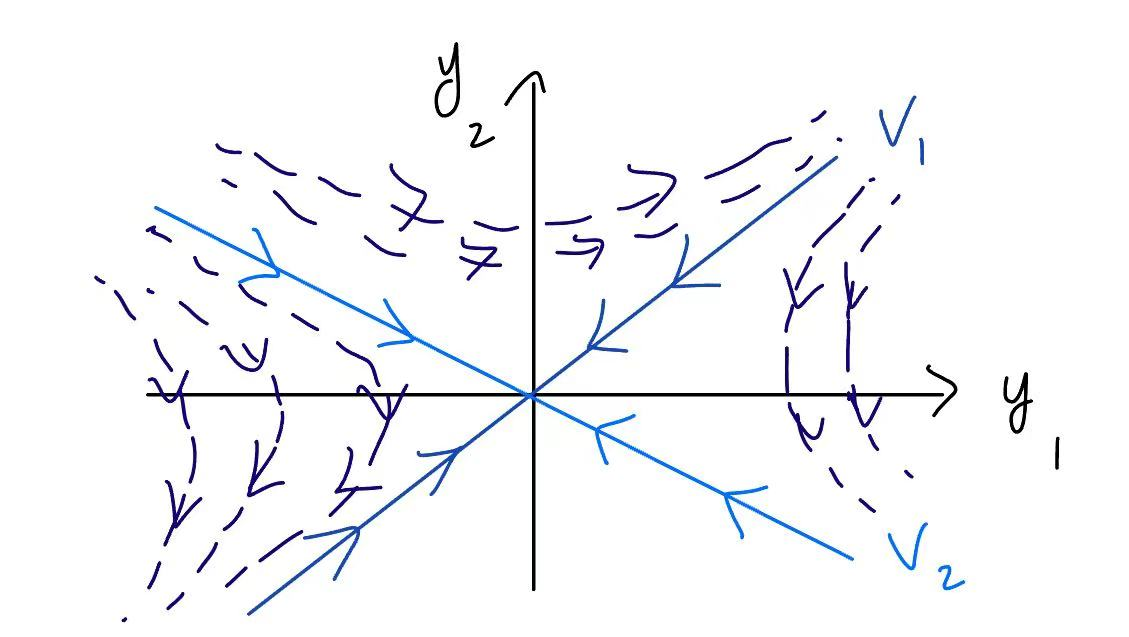
\includegraphics[width=8cm]{DE-ch4-stablesink-2.jpg}
\end{figure}\subsubsection*{Saddle points}
If $\lambda_1, \lambda_2$ are both real but have opposite signs, we obtain a \it saddle point \normalfont as follows:

\begin{figure}[h]
    \centering
    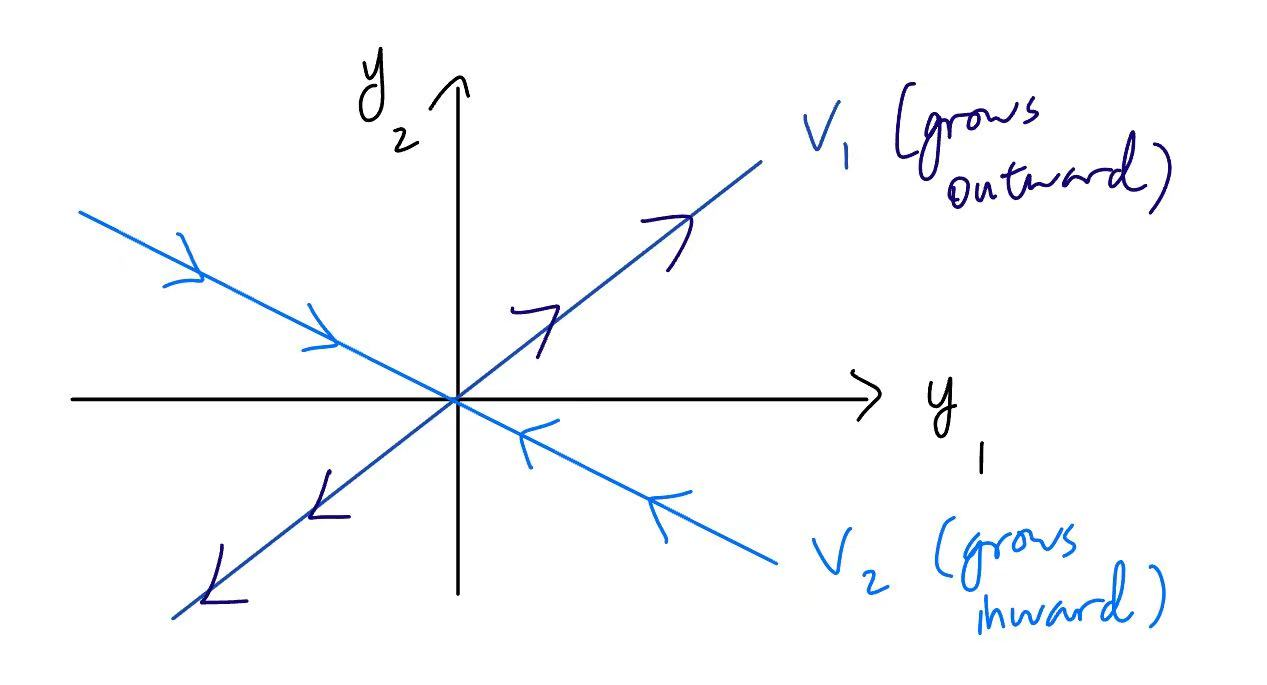
\includegraphics[width=8cm]{DE-ch4-saddlenode.jpg}
\end{figure}

This originates from one of $y_1, y_2$ growing exponentially and the other decaying exponentially. 
\subsubsection*{Spiral points}
If $\lambda_1$, $\lambda_2$ are complex conjugates (they must be, given that they are the solutions to a quadratic equation), we have three different cases. Let $\lambda_{1,2} = a \pm bi$, resulting in $y_{1,2} = e^{ax}(\cos{bx}\pm\sin{bx})$. Then we have a phase portrait that looks like a spiral: 

\begin{figure}[h]
    \centering
    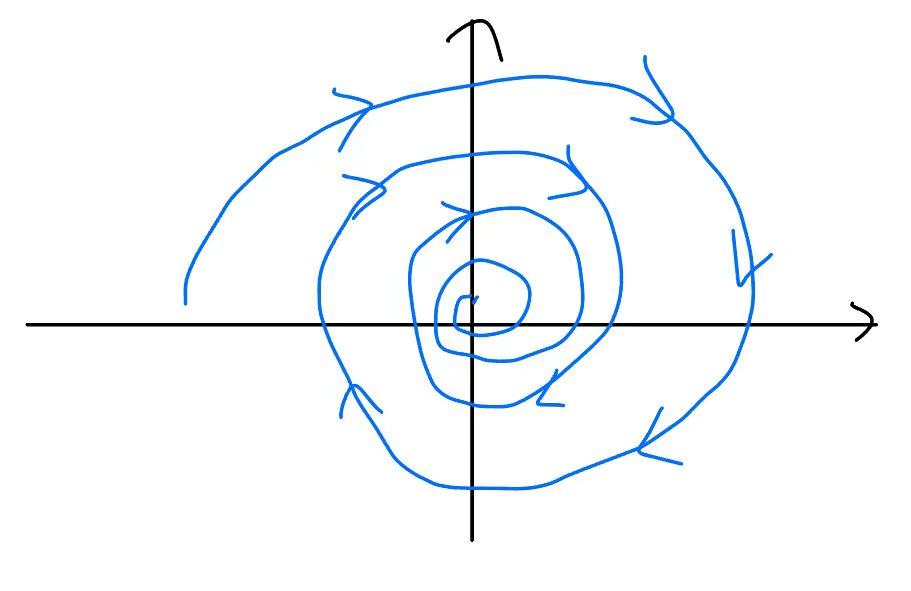
\includegraphics[width=8cm]{DE-ch4-spiral.jpg}
\end{figure}

Why a spiral? Because if we consider the $\cos bx + \sin bx$ term on its own, that multiplied by a vector gives us an ellipse (as we know ellipses have parametric equations $x=a\cos t, y=b\sin t$). But when the $e^{ax}$ term comes in, this "ellipse" either expands exponentially, creating an outward spiral, or collapses inward exponentially, creating an inward spiral. Alternatively, if the real part is zero, the phase portrait is simply two ellipses centered at the origin.
\subsection{Nonlinear dynamical systems}
This section provides an analogue to the technique of stability analysis for a single autonomous ODE, and extends it to a system of ODEs. Consider the second-order system of DEs 
\begin{equation*}
    \begin{cases}
        \dot{x}=f(x,y)\\
        \dot{y}=g(x,y)
    \end{cases}
\end{equation*}
where $x$ and $y$ are functions in $t$. This is an \it autonomous \normalfont system, in the sense that the independent variable $t$ does not appear anywhere in the system. Solving the equations can be nigh-impossible, but through analyzing their fixed points and their stabilities, we can learn many things about them. 
\begin{definition}
    (Equilibrium points.) As with a single equation, we define an equilibrium point or fixed point of a system of ODEs (such as the one shown above) as a point $(x_0,y_0)$ for which $\dot{x}=\dot{y}=0$. 
\end{definition}
We observe that this occurs when $f(x_0,y_0)=g(x_0,y_0) = 0$.\\ \\
To determine the stability of the equilibrium point $(x_0,y_0)$, we consider - as before - a small perturbation $(x_0+\alpha, y_0+\beta)$ from $(x_0,y_0)$. As such we have
\begin{equation*}
    \begin{aligned}
        \frac{d}{dt}(x_0+\alpha)&=\frac{d\alpha}{dt}\text{ (left-hand side)} \\
        &=f(x_0+\alpha, y_0+\beta)\text{ (right-hand side)} \\ \\
        \frac{d}{dt}(y_0+\beta)&=\frac{d\beta}{dt}\text{ (left-hand side)} \\
        &=g(x_0+\alpha, y_0+\beta)\text{ (right-hand side)}
    \end{aligned}
\end{equation*}
and thus by the multivariate Taylor expansion, we have 
\begin{equation*}
    \begin{cases}
        \frac{d\alpha}{dt} =f(x_0+\alpha, y_0+\beta) \approx f(x_0,y_0)+\alpha \frac{\partial f}{\partial x}(x_0,y_0) + \beta\frac{\partial f}{\partial y}(x_0,y_0)\\
        \frac{d\beta}{dt} =g(x_0+\alpha, y_0+\beta) \approx g(x_0,y_0)+\alpha \frac{\partial g}{\partial x}(x_0,y_0) + \beta\frac{\partial g}{\partial y}(x_0,y_0)
    \end{cases}
\end{equation*}
ignoring all second-order and above terms. As $f(x_0,y_0)=0$ by definition of an equilibrium point, we have 
\begin{equation*}
    \begin{bmatrix}
        \dot{a} \\\dot{b}
    \end{bmatrix}=\begin{bmatrix}
        f_{x} & f_{y} \\
        g_{x} & g_{y}
    \end{bmatrix}\begin{bmatrix}
        \alpha \\ \beta
    \end{bmatrix}
\end{equation*}
which is a system of differential equations that we can analyze using the methods demonstrated above. 
\newpage
\section{Partial differential equations}
The big cheese.\\ \\
Normal equations - the ones we grew up with, ones of the form $x+5=10$ or $2x+3=5$ or "solve for $t$ in $e^{-t} = 0$, where $t$ is the time elapsed before your dad comes back with the milk - describe what things are like now: the $x$ in $x+5=10$, for instance, is equal to $5$ now, and it always will be. Differential equations, in contrast, describe how things change over time; instead of finding a single solution that tells us what it is at that present moment, we have to find a function that, at all times, is related to its own rate of change in some meaningful way - something necessitated in nearly every realm of the real world, from an object whose air resistance depends on its own speed of motion, to a disease which spreads more quickly the more people it infects. \\ \\
So what do partial differential equations do? Things in the real world don't just change based on one variable alone; we live in three dimensions, not two, and the models we need to model that three-dimensional world also needs to be three-dimensional. PDEs give us the ability to express relationships not only through the rate of change of something based on a single variable, but based on multiple variables - space and time, instead of one or the other. 
\subsubsection{The transport equation}
We begin our discussion of PDEs with a generalized example that can describe many different situations: a wave traveling in one direction. What do we mean by "wave", in this case? As an example, consider two people holding a rope. When one person jiggles the rope a little bit, there's going to be a displacement that occurs on that person's end:
\begin{figure}[h]
    \centering
    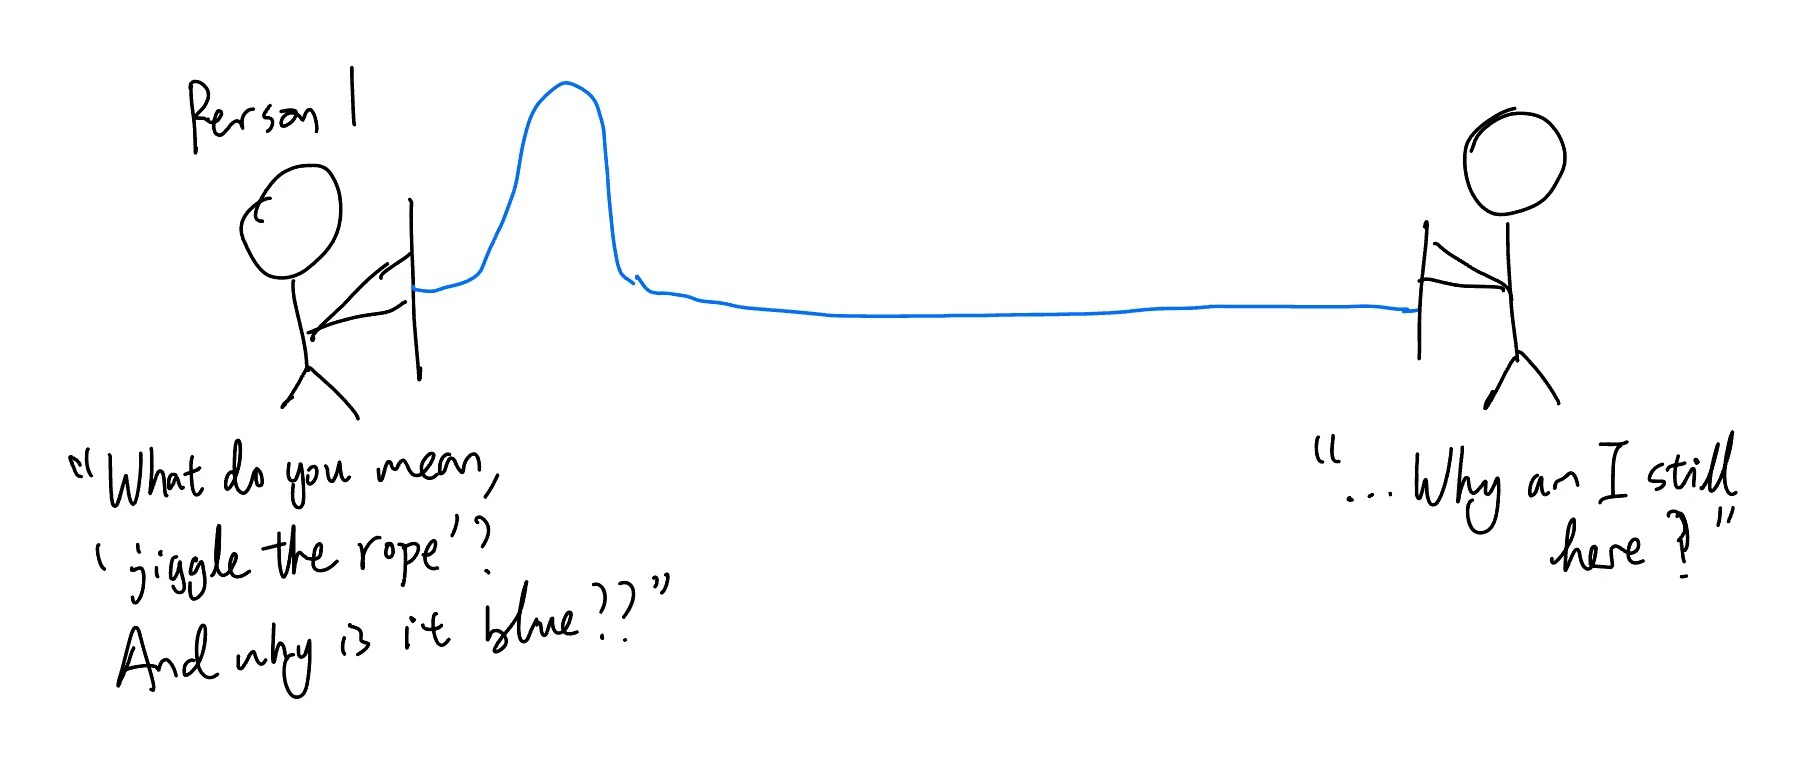
\includegraphics[width=12cm]{DE-ch4-transportequation-1.jpg}
\end{figure}
Naturally, this disturbance on the rope is going to travel forward and reach the other person as time elapses:
\newpage
\begin{figure}[h]
    \centering
    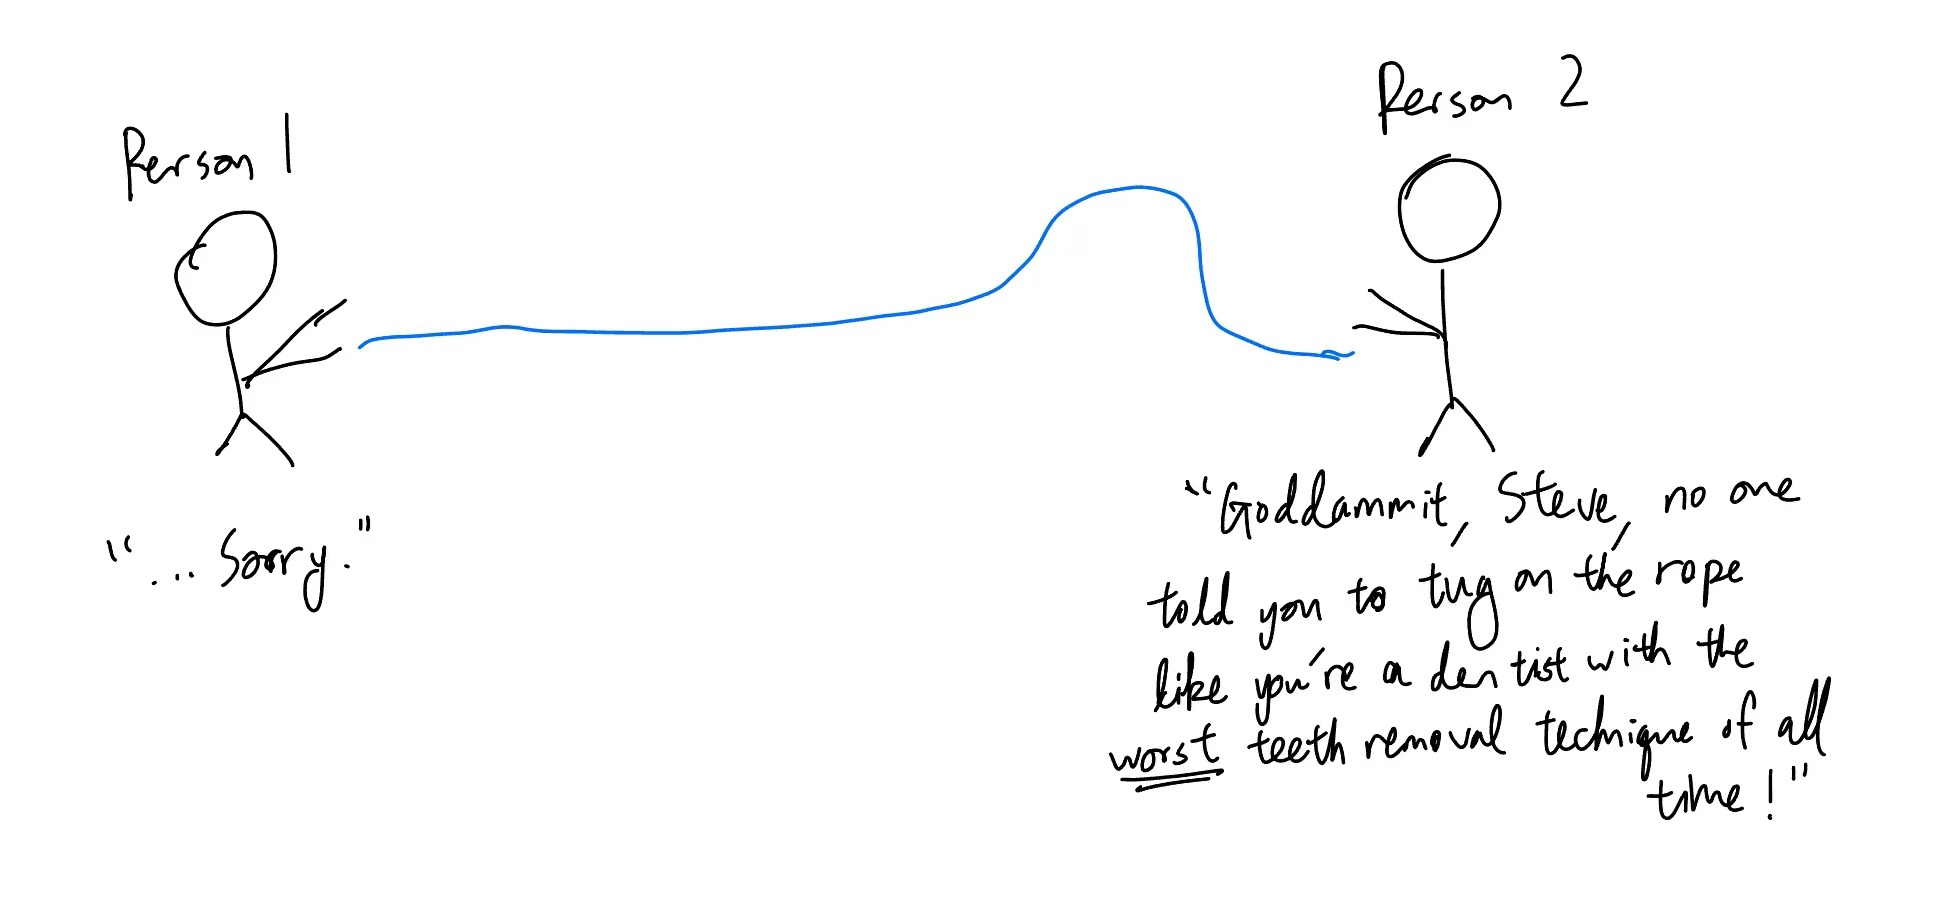
\includegraphics[width=12cm]{DE-ch4-transport2.jpg}
\end{figure}
What we mean by a "wave" is just any function - say a function with displacement $u$ at position $x$ - that travels forward as the time $t$ increases, much like how the "ripple" on the rope travels forward from left to right. \\ \\
Suppose that this wave had speed $c$; that is, if at one moment you had a point on the wave with position $x=x_0$ and displacement $u$, then $t$ seconds later, the same point would have travelled to position $x_0 + ct$ instead. 
\begin{figure}[h]
    \centering
    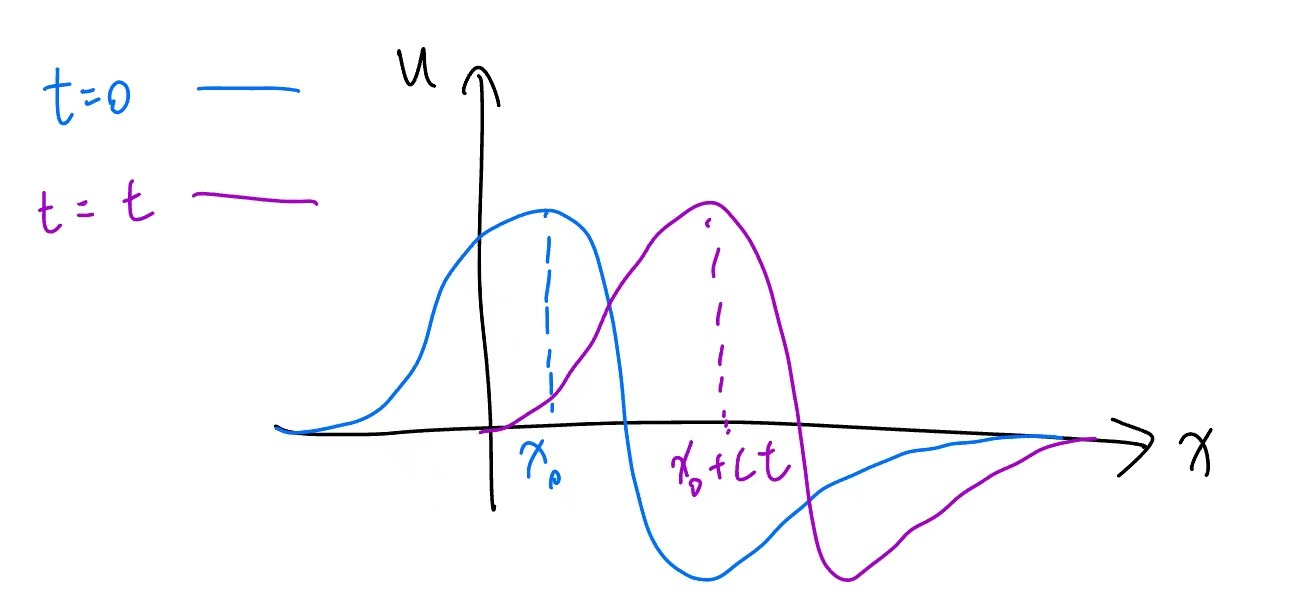
\includegraphics[width=8cm]{DE-ch4-transport3.jpg}
\end{figure}\\
At any one value of $t$, the wave has a single graph: you can say with certainty that, for every value of $x$, we have one displacement $u$. But as $t$ increases, the graph begins shifting to the right at a rate dictated by the speed of the wave $c$. As such, we can model a wave traveling forward as an infinite collection of graphs for $u$ against $x$, one for each value of time $t$, each being identical to the other except for being shifted to the left or right by a certain number of units ($ct$ units) - a multivariate function $u = f(x,t)$. \\ \\
What does this mean for us? Most importantly, it means that if we are traveling alongside the wave - if we also travel at a speed $c$, and in the same direction as the wave - we will not see the graph of the wave changing. For example, let's say we start at the peak of the wave, at position $x=0$; three seconds pass, and by now, the peak of the wave is at position $x=3c$ for some wavespeed $c$. However, we are also traveling at a speed $c$, so three seconds later, we are also at $x=3c$; and thus we again see the peak of the wave, and nothing has changed. \newpage
\begin{figure}[h]
    \centering
    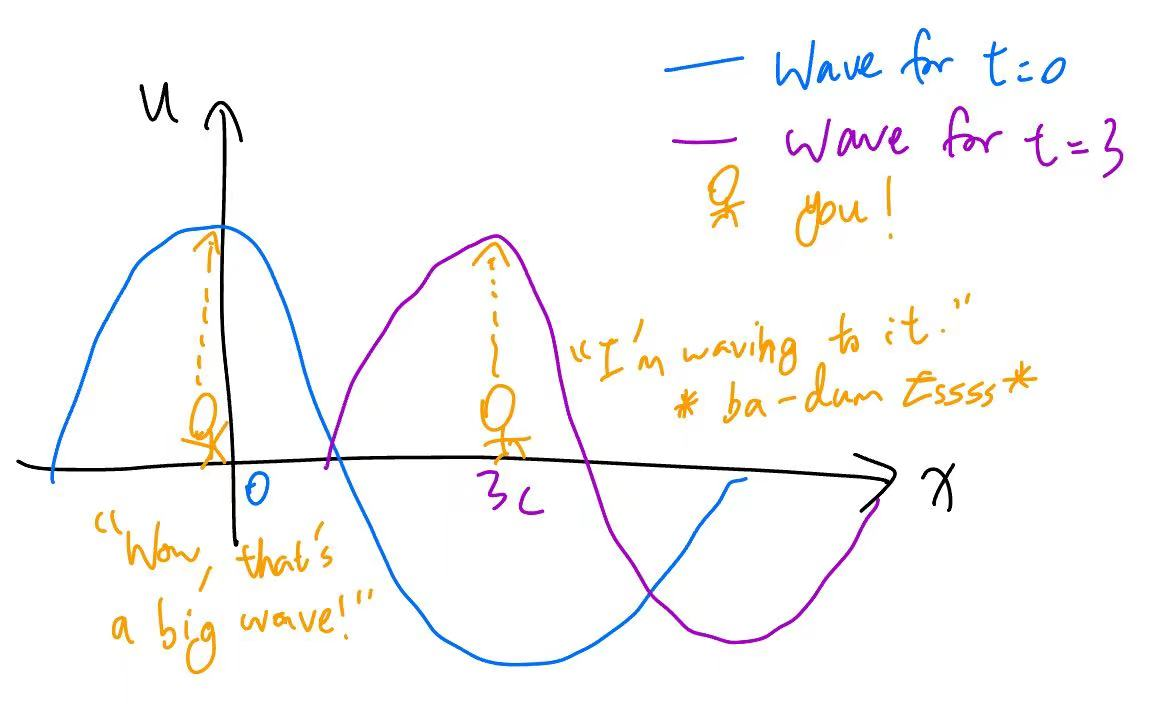
\includegraphics[width=8cm]{DE-ch4-transport4.jpg}
\end{figure}

This means that, if we travel in the direction $x = x_0 + ct$ - if we travel at a speed of $c$, increasing our position $x$ by $c$ units every 1 unit of time $t$ - we will experience no change in the displacement of the wave $u$. In essence, if we keep up with the speed of the wave, the wave will look like it isn't changing at all; in differential-equation terms, its directional derivative along the direction we are traveling, $\begin{bmatrix}
    c\\1
\end{bmatrix}$, is zero:
\begin{equation*}
        \begin{bmatrix}
            c\\1
        \end{bmatrix}\cdot \begin{bmatrix}
            u_x \\ u_t
        \end{bmatrix} = 0
\end{equation*}
yielding the \it transport equation\normalfont 
\begin{equation*}
    u_t+cu_x=0.
\end{equation*}
\begin{definition}
    (Transport equation.) The \it transport equation \normalfont describing waves that transport energy in one direction is given by \begin{equation*}
        u_t+cu_x=0.
    \end{equation*}
    where $u(x,t)$ is the displacement of the wave, $x$ is its position, $t$ the time elapsed, and $c$ the wave speed.
\end{definition}
In basic terms, this equation encodes the information that the dot product between the gradient and the direction $[c,1]$ - the direction of traveling at a constant speed $c$ in the $x$-direction - is zero; the displacement of the wave does not change if you travel in that direction.\\ \\
How do we go about solving this equation? The crux of the matter again relies on the fact that the lines $x-ct=x_0$ are "\it characteristic lines\normalfont" of the transport equation - they are lines where the function $u$ does not change at all with respect to time: $\frac{\partial u}{\partial t}=0$. If we move along these lines $x = x_0 + ct$, then $u(x,t)=u(x_0+ct, t)$ - a function in $t$ only - and we know that $\frac{\partial u}{\partial t}=\frac{du}{dt}=0$.\\ \\
(We can verify this with a little calculation. $\frac{du}{dt} = \frac{\partial u}{\partial t}\frac{\partial t}{\partial t} + \frac{\partial u}{\partial x}\frac{\partial x}{\partial t} = \frac{\partial u}{\partial t} + c\frac{\partial u}{\partial x} = u_t+cu_x$, as $\frac{\partial x}{\partial t}$ is $\frac{\partial}{\partial t} (x_0+ct)=c$. This is simply the transport equation, which we know to be zero, so $\frac{du}{dt}=0$.)
\\ \\
Thus we have the system of ordinary differential equations 
\begin{equation*}
    \begin{cases}
        \frac{\partial u}{\partial t} = 0 \\
        x = x_0 + ct
    \end{cases}
\end{equation*}
From the first equation, we know that $u$ is independent of $t$ along $x = x_0 + ct$ and only depends on $x$: $u = f(x)$. Substituting the second equation gives 
\begin{equation*}
    u=f(x_0+ct)
\end{equation*}
as our general solution for any function $f$ that is differentiable, or simply $u=f(x+ct)$ as $x_0$ is not fixed and can be any value of $x$. If the initial condition $u(x,0)=g(x)$ is imposed, then we have $u=g(x+ct)$.
\subsubsection{The wave equation}
The transport equation gave a general model of a function that moved forward without changing its shape; for each value of $t$, the graph for the shape of the wave was identical barring a translation to the left or right. But in real life, many examples of waves do not simply translate; they also oscillate up and down as they translate forward, necessitating the use of another model. For instance, see the following animation:
\begin{frame}{Wave visualization.}
    \animategraphics[loop,controls,width=\linewidth]{10}{DE-ch4-wave1-}{1}{59}
\end{frame}

(All credit goes to the excellent responses at \hyperlink{https://math.stackexchange.com/questions/1812922/help-visualizing-solutions-to-the-1d-wave-equation}{Math Stack Exchange!})
\\ \\
As we can see, the red wave and the blue wave are both examples of solutions to the transport equation: they translate forward, but the graphs do not oscillate. The magenta wave, however, is an example of a solution to the wave equation: as it travels forward, its peaks and troughs oscillate and constantly change. \\ \\
The question is, what physical laws govern these oscillations? We know based on intuition that at the wave's peaks, there should probably be a \it restoring force \normalfont pulling the wave downwards towards the zero-line, and at its troughs (bottom points), there should also be a force pulling the wave up.
\newpage
\begin{figure}[h]
    \centering
    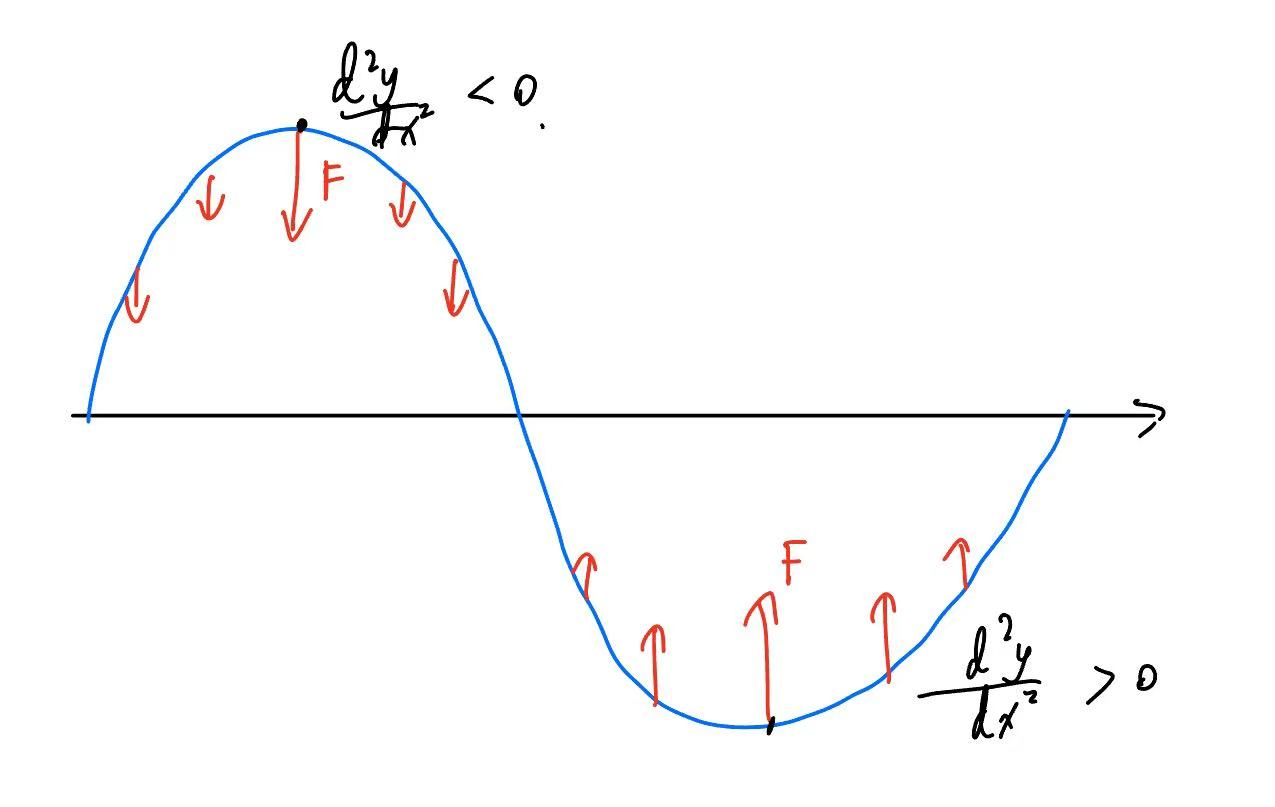
\includegraphics[width=10cm]{DE-ch4-wave2.jpg}
\end{figure} 
When the wave is below the horizontal axis, the concavity (second derivative) is positive, as the gradient of the wave is increasing; when the wave is above the horizontal axis, the concavity is instead negative. This leads us to the hypothesis that the force on each point of the wave is proportional to the concavity of the point, or its second derivative; in other words, 
\begin{equation*}
    \frac{\partial^2 u}{\partial t^2} = k\frac{\partial^2 u}{\partial x^2}
\end{equation*}
for some constant $k$, where $u$ is the displacement of the wave (in a vertical direction), $u_{tt}$ is the second derivative with respect to time and thus the acceleration of the wave (proportional to the force on the wave, by Newton's Second Law), and $u_{xx}$ is the second derivative of the wave with respect to its horizontal displacement - in other words, its concavity along the $x$-axis.\\ \\ 
This is a reasonable enough hypothesis, and it turns out we have enough information to prove it rigorously. Let's consider a tiny segment of the wave as follows, and make the following three assumptions:
\begin{enumerate}
    \item This small section of the wave is nearly perfectly straight. \sout{That means you won't see it making a profile on Grindr anytime soon}
    \item The angle of the section to the horizontal can be modelled by a function of $x$ and $t$, $\theta(x,t)$, which is nearly zero but not constant.
    \item The vertical displacement of this small section is fairly small; we can make this assumption because the section itself is infinitely small, so the force acting on it will be of a similar magnitude. In other words, this small section of the wave is assumed to be nearly horizontal; if we take $\theta$ to be its angle with the horizontal, then its slope, $\tan \theta$, is very close to $\sin \theta$ (as $\cos \theta \approx 1$). 
    \item There are no external forces acting on the wave, only the force of its own tension $T(x,h)$ (if we imagine the wave to be a string); in other words, the wave or string is perfectly flexible.
    \item The density of the section is constant: $\rho(x,t)=\rho$.
\end{enumerate}
A visualization of this is shown below:
\newpage
\begin{figure}[h]
    \centering
    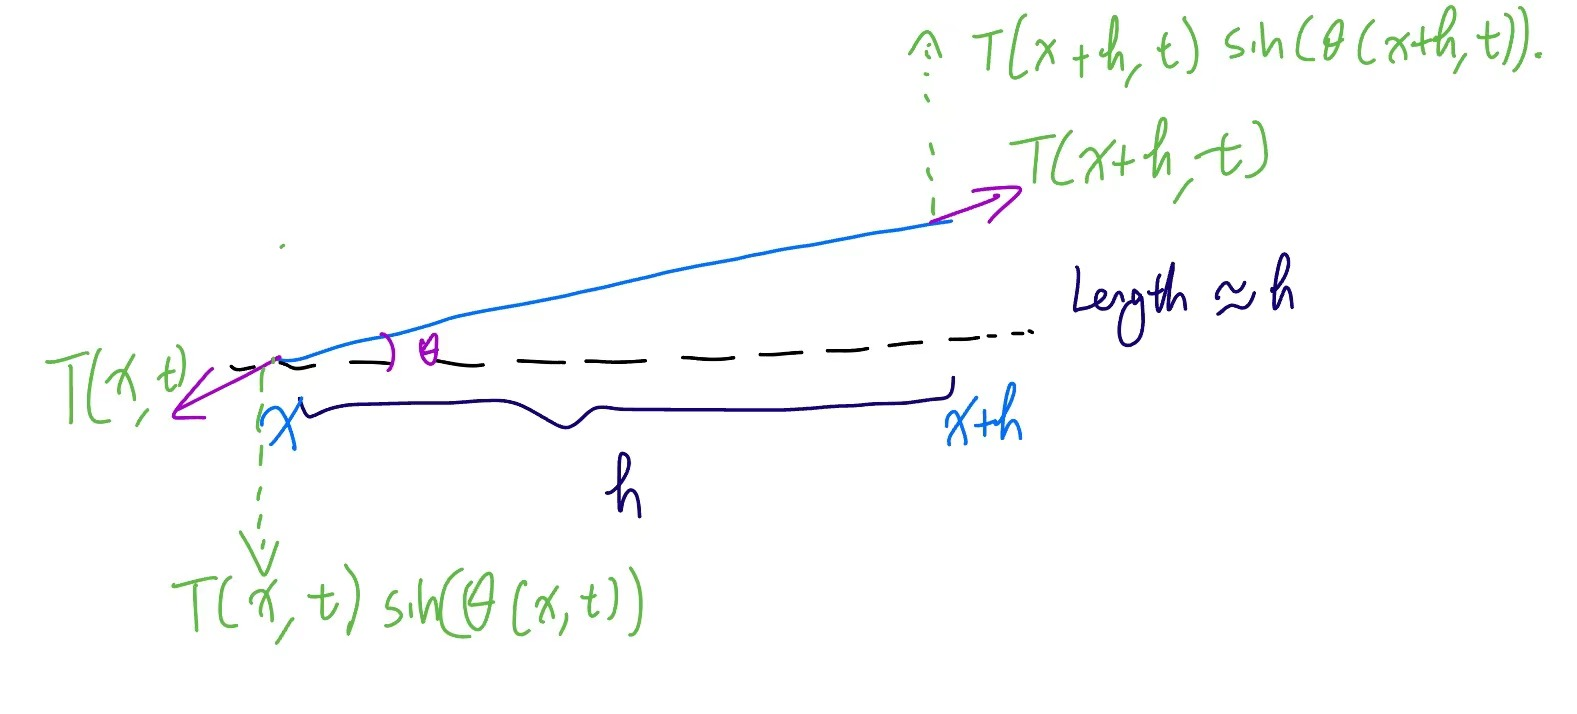
\includegraphics[width=12cm]{DE-ch4-wave3.jpg}
\end{figure}

Let the starting point of the section be $(x,t)$ and the endpoint be $(x+h,t)$. The length of the section, being nearly horizontal, is approximately $h$. By Newton's Second Law, we know that the net force on the section is equal to $ma = mu_{tt}=\rho h u_{tt}$. There are no other forces acting on the section other than tension, so the net force is simply 
\begin{equation*}
    T(x+h,t)\sin(\theta(x+h,t))-T(x,t)\sin(\theta(x,t))
\end{equation*}
or the vertical component of the tension at the endpoint, subtracted by the vertical component of the tension at the starting point. The horizontal components can be assumed to be equal and opposite (since $T$ and $\theta$ change negligibly from $x$ to $x+h$). Thus, we write 
\begin{equation*}
    T(x+h,t)\sin(\theta(x+h,t))-T(x,t)\sin(\theta(x,t)) = \rho h u_{tt}
\end{equation*}
or, equivalently, dividing by $h$ obtains 
\begin{equation*}
    \frac{T(x+h,t)\sin(\theta(x+h,t))-T(x,t)\sin(\theta(x,t))}{h} = \rho u_{tt}
\end{equation*}
where, by first principles of derivatives, the left-hand side is equal to 
\begin{equation*}
    \frac{\partial}{\partial x}(T(x,t)\sin\theta(x,t))
\end{equation*}
The pesky fact of the matter here is that we have a $\sin \theta$ term that we do not want. As we stated earlier, however, the slope of our section (which can also be written $u_x$, since the section is infinitely small) is equal to $\tan \theta(x,t)$, which, when $\theta$ is very small, is approximately equal to $\sin \theta(x,t)$. Thus, the above expression is equivalent to 
\begin{equation*}
    \frac{\partial}{\partial x}(T(x,t)u_x)
\end{equation*}
which, when we assume that tension is constant throughout the section, leaves us with simply
\begin{equation*}
    Tu_xx=\rho u_{tt}
\end{equation*}
or 
\begin{equation*}
    c^2 u_xx= u_{tt}
\end{equation*}
where $c$ is a constant. (We can show that $c$ is actually equal to the speed of the wave by means of dimensional analysis; $u_xx$ has dimensions $m^{-1}$, $u_{tt}$ has $m\ s^{-2}$, and thus their ratio is of dimension $m^2\ s^{-2}$ - the square of $m\ s^{-1}$.) This gives us our desired wave equation. \\ \\
The solution to the wave equation is motivated by its connection to the transport equation. To start with, we need to ask ourselves: does a solution to the transport equation satisfy the wave equation? Intuitively it does, since the solution to the transport equation is simply a wave with no oscillation at all, and should still satisfy the wave equation. To verify this, let's assume that 
\begin{equation*}
    cu_x + u_t=0
\end{equation*}
such that some $u(x,t)$ satisfies the transport equation. We know that $u(x,t)$ is in the form $f(x+ct)$; this is the forward transport equation. Thus, we have 
\begin{equation*}
    u_{tt}=c^2f_{tt}(x+ct)=c^2 u_{xx}
\end{equation*}
Therefore, the transport equation solves the wave equation too. But to obtain general solutions, we need another function $g$ that can create oscillations on top of the function $f$, which just moves forward without oscillating. This can happen if $g$ is a wave also satisfying the transport equation, but moving in the opposite direction; this way, the two waves will interfere due to superposition. Thus we have 
\begin{equation*}
    g(x-ct)
\end{equation*}
as the second term of our solution; we can quickly verify that $g(x-ct)$ also solves the wave equation. Thus, our complete solution is 
\begin{equation*}
    u=f(x+ct)+g(x-ct)
\end{equation*}
for any differentiable functions $f$ and $g$; essentially, the solution to the wave equation is two waves described by the transport equation moving in opposite directions. (Quickly verifying this by plugging this back into the wave equation yields the system of equations 
\begin{equation*}
    \begin{cases}
        u_{t}+cu_x=g \\
        g_t-cg_x=0
    \end{cases}
\end{equation*}
which gives back $u=f(x+ct)+g(x-ct)$. \\ \\
To prove that this is the most general solution, we observe that we can write the wave equation as 
\begin{equation*}
    \frac{\partial^2 u}{\partial t^2} - c^2\frac{\partial^2 u}{\partial x^2} = (\frac{\partial}{\partial t} + c\frac{\partial}{\partial x})(\frac{\partial}{\partial t} - c\frac{\partial}{\partial x})u = 0
\end{equation*}
And thus $u$ solves either $u_t+cu_x=0$ or $u_t-cu_x=0$, yielding the previous two solutions.

(For a visualization of how the solutions to the wave equation arise from two solutions to the transport equation in opposite directions, see the animation above.)
\subsubsection{The heat equation}
The heat equation, or the diffusion equation, models the conduction of heat throughout a solid (in one dimension only, though it is possible to generalize to more dimensions). To understand it, let us consider the case of a 1D metal rod with zero (or negligible) thickness, and some length $L$. Let the temperature of the rod at any given point $x$ along the rod at a time $t$ be $T(x,t)$, such that $T(x,0)$ describes the temperature distribution of the rod at time $t=0$, $T(x,1)$ at $t=1$, and so on:
\begin{figure}[h]
    \centering
    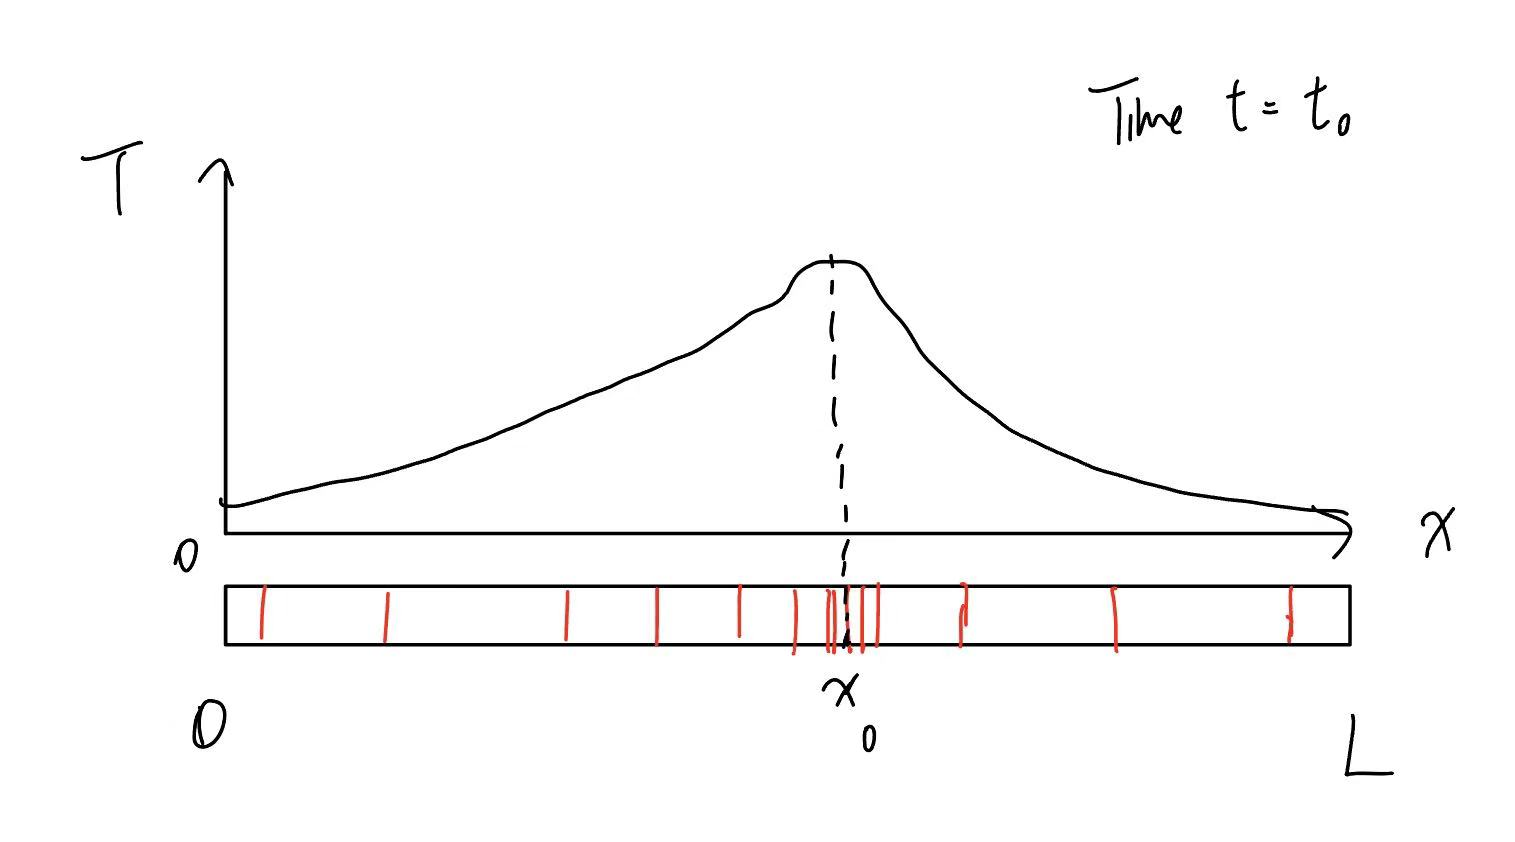
\includegraphics[width=10cm]{DE-ch4-heat1.jpg}
\end{figure}
At time $t_0$, every point on the rod has a temperature $T(x)$, and the value of $T(x)$ is expressed on the plot above. If we combine such plots for every value of $t$, we obtain something as follows:
\begin{figure}[h]
    \centering
    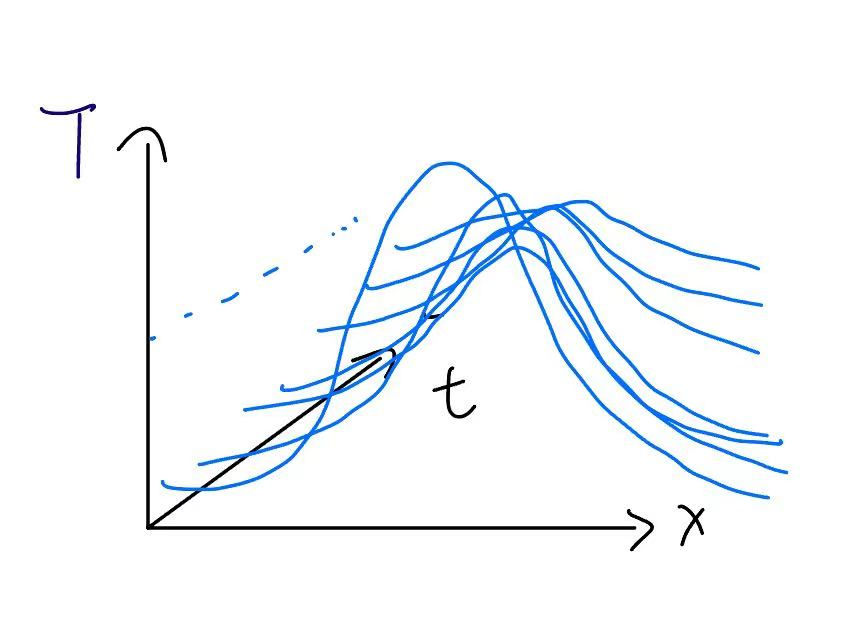
\includegraphics[width=8cm]{DE-ch4-heat2.jpg}
\end{figure}
Intuition tells us that as time elapses, the graph will "flatten out" (as shown above); heat will disperse evenly throughout the rod. If we can codify that sense of intuition into the language of differential equations, we'll have our heat equation. To do that, let's consider a discrete, rather than continuous, version of the rod. Say, for instance, that we are measuring the temperature of the rod at ten distinct points:
\newpage
\begin{figure}[h]
    \centering
    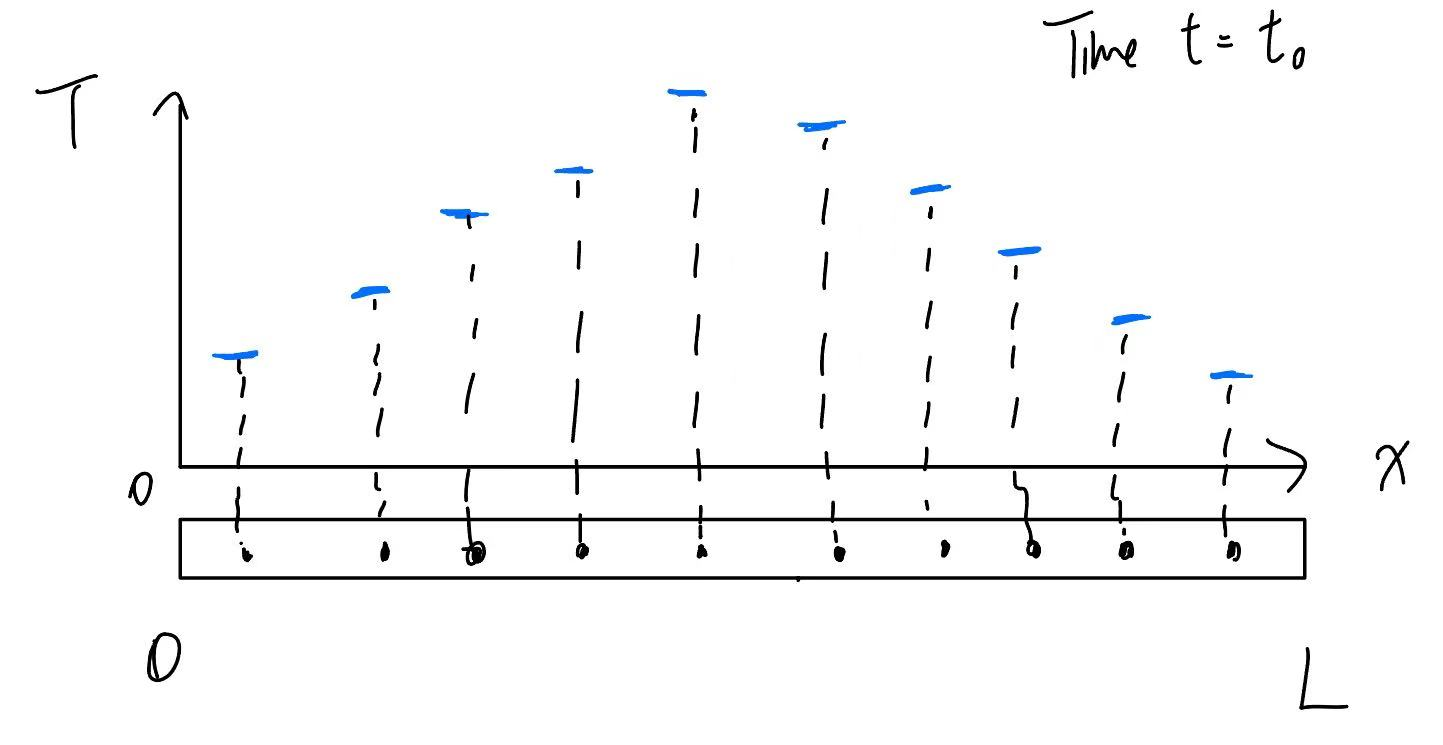
\includegraphics[width=10cm]{DE-ch4-heat3.jpg}
\end{figure}
Let's consider only the behavior of a single point:
\begin{figure}[h]
    \centering
    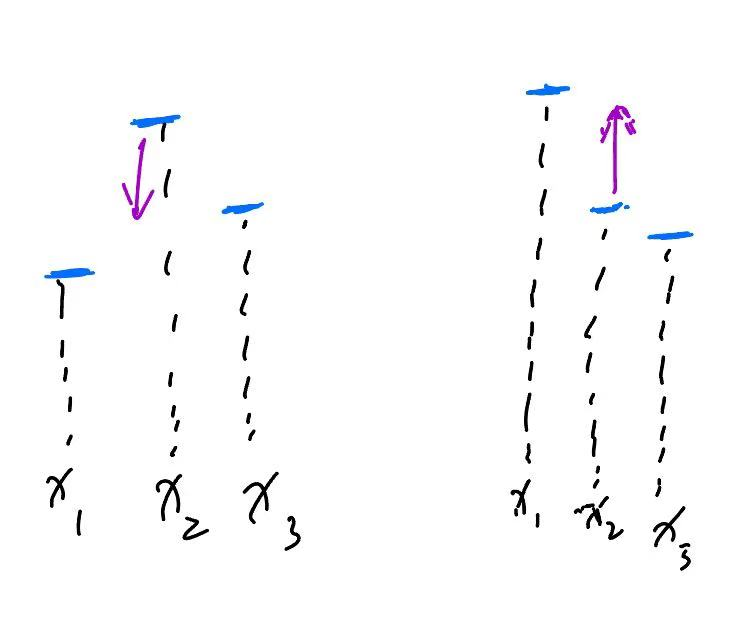
\includegraphics[width=8cm]{DE-ch4-heat4.jpg}
\end{figure}

On the left-hand case, the point $x_2$ has a higher temperature than both of its neighbors $x_1$ and $x_3$, telling us that its temperature will tend to decrease; on the right-hand case, though $x_1$ has a higher temperature than $x_2$ and $x_3$ has lower, the average of $x_1$ and $x_3$ still exceeds $x_3$, making it tend to increase in temperature. Thus, we can write that for a discrete point $x_2$ on the rod with temperature $T(x_2,t)$, the rate of change of its temperature is proportional to the average of its temperature difference with its neighboring points:
\begin{equation*}
    \frac{\partial T}{\partial t} = \alpha(\frac{(T_3-T_2)-(T_2-T_1)}{2})
\end{equation*}
for a certain proportionality constant $\alpha$. $(T_3-T_2)-(T_2-T_1) = \Delta T_2 - \Delta T_1 = \Delta \Delta T_1$, the \it second difference \normalfont of $T_1$; as the distance between neighboring points becomes infinitesimal, the second difference is analogous to the second derivative with respect to $x$. Thus, we obtain the heat equation: 
\begin{equation*}
    \frac{\partial T}{\partial t}=\kappa \frac{\partial^2 T}{\partial x^2}
\end{equation*}
where $\kappa$ is the \it diffusivity \normalfont of the rod. \\ \\
\newpage
Solutions to the heat equation lie once again in the method of changing variables from $(x,t)$ to a single variable $\eta$ such that the function $T$ can be rewritten entirely in terms of $\eta$: $T(x,t)=T(\eta)$. Note that this is the same method we used with solving the transport equation, where we had $x = x_0 + ct$ which yielded a function entirely in $t$. The question is, what is $\eta$? Unlike the transport equation, there are many, many different possible ways to define $\eta$ as some function of $t$ and $x$ such that it helps us solve the heat equation, so let us consider only one:
\begin{equation*}
    \eta = \frac{x}{2\sqrt{\kappa t}}
\end{equation*}
where $\kappa$ is again the diffusivity. This is known as a \it similarity solution, \normalfont as it only encompasses all solutions which are in exactly this form (can be written in terms of $\eta$) and are similar to one another. If we posit that $T(x,t)$ can be written entirely as $T(\eta(x,t))=F(\eta)$, a single-variable function of $\eta$, then we have
\begin{equation*}
    \begin{cases}
        \frac{\partial T}{\partial x} = \frac{\partial F}{\partial \eta} \frac{\partial \eta}{\partial x} \\
        \frac{\partial T}{\partial t} = \frac{\partial F}{\partial \eta} \frac{\partial \eta}{\partial t}
    \end{cases}
\end{equation*}
and with $\eta = \frac{x}{2\sqrt{\kappa t}}$, we have 
\begin{equation*}
    \begin{cases}
        \frac{\partial \eta}{\partial x} = \frac{1}{2\sqrt{\kappa t}} \\
        \frac{\partial \eta}{\partial t} = -\frac{\kappa x}{4}(\kappa t)^{-\frac{3}{2}}
    \end{cases}
\end{equation*}
resulting in
\begin{equation*}
    \begin{cases}
        \frac{\partial T}{\partial x} = \frac{1}{2\sqrt{\kappa t}}\frac{\partial F}{\partial \eta} \\
        \frac{\partial^2 T}{\partial x^2} = \frac{1}{2\sqrt{\kappa t}}\frac{\partial^2 F}{\partial \eta^2} \frac{\partial \eta}{\partial x} = \frac{1}{4\kappa t}\frac{\partial^2 F}{\partial \eta^2} \\
        \frac{\partial T}{\partial t} = \frac{\partial F}{\partial \eta} \frac{\partial \eta}{\partial t} = -\frac{\kappa x}{4}(\kappa t)^{-\frac{3}{2}}\frac{\partial F}{\partial \eta} = -\frac{1}{2}\frac{x}{2\sqrt{\kappa t}t}\frac{\partial F}{\partial \eta} = -\frac{\eta}{2t}\frac{\partial F}{\partial \eta}
    \end{cases}
\end{equation*}
Substituting this into the original heat equation yields
\begin{equation*}
    \begin{aligned}
        -\frac{\eta}{2t}\frac{dF}{d\eta}&=\frac{1}{4t}\frac{d^2F}{d\eta^2} \\
        \frac{d^2F}{d\eta^2}+2\eta\frac{dF}{d\eta}=0
    \end{aligned}
\end{equation*}
which solves to obtain $\frac{dF}{d\eta} = Ae^{-\eta^2}$ and thus the non-elementary $F=\alpha\ \text{erf}(\eta) + \beta$ for the error function erf, defined as 
\begin{equation*}
    \text{erf}(\eta)=\frac{2}{\sqrt{\pi}}\int_{0}^{\eta}e^{-u^2}\ du
\end{equation*}
\end{document}